\documentclass{article}

\usepackage{csvsimple}
\usepackage{graphicx}
\usepackage{caption}
\usepackage{subcaption}
\usepackage{hyperref}
\usepackage{listings}
\usepackage{url}
\usepackage{hyphenat} % hyphenation of underscores

\begin{document}

\title{
    Assignment 2 - Language detection using Copy Models for compression \\
    \large{Algorithmic Information Theory (2022/23) \\
    Universidade de Aveiro}
}

\author{
    Martinho Tavares, 98262, martinho.tavares@ua.pt \and
    Nuno Cunha, 98124, nunocunha@ua.pt \and
    Pedro Lima, 97860, p.lima@ua.pt
}

\date{\today}
\maketitle

\section{Introduction}
\label{sec:introduction}

The goal of this assignment is to implement a language detection system using the previously developed copy model from the last assignment.
The system is capable of detecting the language of a given text, if it is one of the languages used to train the model.
To implement this, a new version of the copy model was developed, called \texttt{lang}, which receives a reference text to train the model and a target text to compress by copying from the reference.
The main idea is that if we use a reference text of a given language then we should get a better compression if the target text matches the provided language, since the same language patterns are to be expected, and so better copies can be made.
If using multiple references, we can comparatively identify a language, by checking which of them provided a better compression of the target text.

One of the other new features implemented in the \texttt{lang} model is the ability to use a finite-context model for the probabilities of non-hit symbols, instead of using the uniform or frequency probability distributions.

With the new model implemented, two other scripts were developed to test its performance and obtain the language prediction in an entire text file or in specific sections of a text.
The first script is called \texttt{find\_lang}, which receives a target text and uses all the existing references to predict the language of the target text, returning the language with the highest probability of being the target's language.
This is done by executing the \texttt{lang} model for each reference text and comparing the total compressed information obtained for each language, returning the reference language that reported the lowest information.

The second script is called \texttt{locate\_lang}, which receives a target text and, like the \texttt{find\_lang} script, executes the lang model for each reference text, but instead of returning the language with the lowest information, it returns the language with the lowest information for each section of the target text.
This is done by saving which language has the lowest information for each step/character of the target text, and then checking the intervals where the language is the same, returning the language that reported the lowest information for each interval.

In this report we will present the methodology used to implement the \texttt{lang} model, the \texttt{find\_lang} and \texttt{locate\_lang} scripts in detail in section \ref{sec:methodology}, and the results obtained by testing the scripts with different target texts in section \ref{sec:results}.
And finally, in section \ref{sec:conclusion}, we will present the conclusions of this assignment.

All code and files used for training and testing are present in the repository\footnote{\url{https://github.com/NMPC27/TAI-G7-Lab2}}.

\section{Methodology}
\label{sec:methodology}

For the development of the different components, we utilized different approaches.
The \texttt{lang} model was written in C++, extending and improving the copy model program developed in the previous assignment.

However, the \texttt{find\_lang} and \texttt{locate\_lang} scripts were developed in Python.
These scripts essentially perform many independent runs of the \texttt{lang} model using different references, and parse the output as they desire.
Since practically all of the heavy processing is performed by the \texttt{lang} model, we can afford the loss of performance that running a script in Python entails in turn for the much increased development simplicity.
In fact, in practice we noticed that most of the execution time spent on these scripts is in the \texttt{lang} model, as the result processing in Python is relatively simple.
For both scripts, parameters of the \texttt{lang} model can be specified.

Even then, \texttt{find\_lang} and \texttt{locate\_lang} take too much time waiting for the results of the \texttt{lang} model.
Therefore, to ease this large bottleneck, we added support for multiprocessing to both of these scripts.
Since different \texttt{lang} models with different references can be run completely independently, without any need of interprocess communication, we can easily launch multiple processes.
The ideal option would be to integrate multithreading directly into the \texttt{lang} model program itself, in C++, which allows greater memory efficiency as the target text doesn't have to be stored in memory multiple times, one for each process.
However, we decided to simply opt for multiprocessing, since multithreading would heavily complicate the source code of the \texttt{lang} model, and also because multiprocessing provided a performance boost good enough for our purposes.
This allowed us to dedicate more time in other areas of the assignment, such as improving the \texttt{lang} model and the scripts.

If, while performing multiprocessing, any of the processes fails for some reason, then the script by default exits outputting the obtained error from the failed process.

In each of the following sections, we provide further development details on each of the components.

\subsection{Lang model}
\label{subsec:methodology_lang_model}

The developed \texttt{lang} model is heavily based on the copy model built for the first assignment.
The major change was adapting the existing program to train a copy model on a given reference text and only then perform predictions on a given target text, instead of performing both training and predicting on a single message.
This allows estimation of the number of bits required to compress the target text using copies from the reference text.

For the \texttt{lang} program, the following changes were done from the first assignment's copy model:
\begin{itemize}
    \item UTF-8 support:
    We are using multiple kinds of languages as references.
    As such, the ASCII encoding used in the first assignment's copy model is not enough to correctly represent the symbols of every language, since not all alphabets fit in that encoding.
    The code would have worked perfectly for UTF-8 text, as it just effectively handled bytes.
    However, it would cut some symbols off, which would make it harder to debug and visually analyze the behaviour of the copying.
    Therefore, we changed the code to support UTF-8 text, now handling symbols as wide \textit{chars} instead of \textit{chars} and strings as \textit{wstrings}.
    
    \item Repeat-like wrapping for the past initialization:
    Since we want to start training/copying since the very first symbol in the reference/target message, we need to consider some kind of context when at that symbol, i.e. we need to somehow train and test the model using the first $k$ symbols, even if we require $k$ symbols of previous context for each of them, which doesn't naturally exist.
    For the first assignment, the strategy that we followed to solve this problem was to initiale this $k$-sized past with the most frequent symbol in the entire message.
    This was an easy solution to implement, but it is much less appropriate when applied for the specific use case of this assignment.
    Since we are dealing with natural language text, it doesn't make sense to incorporate $k$ repeated instances of a single letter, as that will definitely not occur for a reasonable value of $k$.
    For the first assignment we mainly dealt with a chromossome sequence, but in this case this issue becomes more obvious.

    Therefore, for the lang program we decided to initialize the $k$-sized past using the last $k$ symbols of the message.
    That is, we perform a repeat-like wrapping on the text.
    This way, we ensure the usage of a context in natural language for the first $k$ symbols.
    The difference between both approaches is illustrated in figure \ref{fig:lang_new_past}

    We have to handle the initialization of the past carefully for both the reference and target texts (note that they are in different character arrays in memory).
    When training on the reference text, we initialize its past with its last $k$ symbols.
    For the target text, we require some context for the first $k$ symbols before we start predicting.
    Therefore, we initialize in the same way, using the last $k$ symbols of the reference text.
    As such, it will be as if the target text was concatenated at the end of the reference text.
    
    \item Usage of \texttt{string\_view}:
    In the previous assignment, we used strings to represent the $k$-sized context/window as we advanced on the text.
    For the copy model itself, we had an hash table whose keys were these $k$-sized windows, i.e. $k$-sized strings.
    This had the disadvantage that, effectively, the entire content of the message being trained on would be reflected in the keys of this hash table.
    Since the message itself is already being stored in memory, the storage of keys in the hash table will increase the amount of memory that the message's content ends up occupying.
    Additionally, advancing through the text involved altering the current $k$-sized window by appending the new symbol at the end and removing the oldest symbol at the beginning.
    This operation is not particularly efficient, especially when the string's content already exists and, in practice, all that is being done is advancing a pointer.

    Therefore, we decided to switch these strings to string views.
    String views just require a pointer to the beginning of a string and the string size.
    This allows the \texttt{lang} program to be more memory efficient by simply pointing to the message content that is already in memory, from which copies are made.
    Additionally, this enforces a fixed size for the strings, which for our case makes sense as the size is always a fixed value $k$.
    
    \item Usage of \texttt{unordered\_map}:
    Our previous copy model made heavy use of the \texttt{map} data structure.
    However, this structure enforces order, which we don't take advantage of, and is not the approximation to an hash table that we desired, contrary to \texttt{unordered\_map}.
    As such, in the lang program we changed all uses of the \texttt{map} structure to \texttt{unordered\_map}, with noticeable improvement in performance.
    
    \item Removed \texttt{ReadingStrategy}:
    In the first assignment, we initially planned to evaluate different approaches to reading the message from disk: either entirely into memory, or in binary directly from disk in case we could not load the entire message into memory.
    We ended up not exploring different approaches other than storing all the content into memory, and so for the \texttt{lang} model we scrapped the abstraction of a reading strategy, incorporating the functionality that was in the respective classes directly into the \texttt{lang} copy model.
\end{itemize}

\begin{figure}
    \centering
    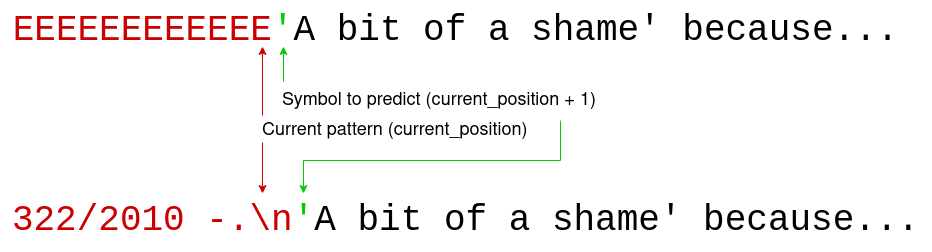
\includegraphics[width=0.95\textwidth]{./images/lang_new_past.png}
    \caption{Illustration of the new past initialization, with the difference between the previous version (above) and the new version (below). The english reference text is used as an example.}
    \label{fig:lang_new_past}
\end{figure}

Other than these changes, various bugfixes and slight optimizations were done on the previous copy model.
Due to the new approach of training and predicting on independent reference and target texts, the code had to be restructured and more responsibilities separated to ensure only training occurs on the reference and prediction is reserved only for the target.

For instance, after training on the reference we have an hash table of the counts of each symbol in the text.
These counts are required by the probability distributions, more specifically the \texttt{FrequencyDistribution}.
However, the probability distributions have to take into account the \emph{target's} alphabet, not the reference's.
Therefore, after performing the initial pass over the target text to determine its alphabet, these counts are updated to remove any symbols that did not appear in the target text and include those that appeared in the target text but not in the reference.
These new symbols, that didn't previously have counts, will have their counts initialized with 1 to avoid reporting an infinite amount of information for them.
Do note that, after passing over the target text, the counts of the symbols both in the reference text and target text are not updated, i.e. only counts actually done on the reference text are used.
This is done because it doesn't make much sense to include the symbol counts on the target text when the objective of the program is to compress solely based on a model trained on a reference text.
Additionally, we mainly want to use this program to compare compression of one same target text using many different references, and so it is not relevant to include the target symbol counts since they would be the same between all runs.

Another note worth making is that most copy pointer managers, which are the copy model components responsible for determining which copy pointer to use at each context, provide the exact same copy pointer repositioning result for a given context, independently of when it is done while predicting.
This is because the array of copy pointers to choose from does not change while traversing the target text anymore, only during training on the reference.
As such, \texttt{NextOldestCopyPointerManager} is the only manager whose copy pointer repositioning behaviour changes for a given context while predicting on the target.

\subsubsection{Verbose modes}
\label{subsubsec:methodology_lang_model_verbose}

The \texttt{lang} program was required to output the total number of bits estimated to be necessary to compress the target text based on the reference text.
To simplify output analysis by the \texttt{find\_lang} script, we added the minimal verbose mode specified with the parameter \texttt{-v o}, which simply prints to standard output nothing more than the total number of bits required for compression.

Additionally, for the \texttt{locate\_lang} script, we needed to know what was the reported information content in bits for each symbol in the target, to correctly identify in which language was each text segment.
Therefore, we modified the previous ``machine'' verbose mode, specified with the parameter \texttt{-v m}, which used to print the whole probability distribution in CSV format to standard output.
This output was previously saved to disk using shell redirection, and since the CSV format was very wasteful in terms of space a lot of disk memory was necessary for these files.

Since now we are only concerned with the probability of the actual symbol in the message, we only need one of those values of the probability distribution at every step.
As such, we opted to instead of printing the floating-point probability values to standard output, to write them directly in sequence to a file in binary format.
This allows for a densely-packed representation of the probability values over the message since no newlines or separators are used and the values are written in their full binary content instead of a character string representation in digits each occupying a byte, saving tremendously in space when compared with the previous assignment's approach.
We can then load these values in a highly efficient manner from the \texttt{locate\_lang} script using the NumPy library.
Do note that these floating-point values, declared as \texttt{double}, are assumed to occupy 64 bits.

Since the new ``machine'' verbose mode outputs the probabilities to a binary file, we added the possibility to declare to which file they are written, by specifying it as an ``option parameter'': \verb|-v m:X|, where \texttt{X} is the path of the file.
If only \texttt{-m} is passed, then the output is written to \textit{lang.bin} by default.
If the specified file already exists, then a prompt asking for ovewrite permission is presented.

\subsubsection{Finite-context model}
\label{subsubsec:methodology_lang_model_fcm}

We explored the possibility of using a finite-context model, or discrete time Markov chain, as the default distribution to report for the symbols that we did not predict at each step.
In this model, we try to estimate the probability that a symbol occurs after a given $k_f$-sized context by counting occurrences of the symbol after that context in the past.
We allowed this model to have an arbitrary order, i.e. the size $k_f$ of the context used.
We can specify a $k_f \leq k$, where $k$ is the size of the context in the copy model itself.

Since we already had a family of classes representing the reported probability distributions, as subclasses of the \texttt{BaseDistribution} class, then we created the finite-context model as a subclass as well, named \texttt{FiniteContextDistribution}.
Implementation involved keeping track of counts of symbols after $k_f$-sized subcontexts seen while training on the reference text.
For that, we used an hash table with the subcontext as the keys and the symbol counts as the values.
The symbol counts themselves were also implemented using hash tables, with the symbols as the keys and the counts as the values.
These tables are updated at every training step on the reference.

After training, we initialize the internal distribution variable, which contains the probability distribution that is reported at each step when predicting, with zeros for each symbol of the target alphabet.
Then, for every hash table of counts in the hash table of subcontexts, we remove all the counts of the symbols that are not in the alphabet, since they won't be used.

Then, at every single prediction step, we update the internal distribution variable to store the probabilities of every symbol based on the obtained symbol counts for the current $k_f$-sized subcontext in the target text.
The probabilities are obtained using the following formula:

$$
P(e|c) = \frac{N(e|c) + \alpha}{\sum_{s \in \Sigma}{N(s|c)} + \alpha |\Sigma|},
$$

where $e$ is the symbol of which we want to calculate the probability of occurring, $c$ is the subcontext used, $\Sigma$ is the target alphabet, $N(x|y)$ is the count of symbol $x$ after subcontext $y$ and $\alpha$ is a smoothing parameter to avoid probabilities of 0.

In case no counts were obtained for the current $k_f$-sized subcontext, then all counts are treated as 0 and the reported distribution is a uniform distribution.

This implementation requires recalculating, at each prediction step, the probabilities of all symbols at each subcontext found in the target text.
If we found the same subcontext multiple times, then the distribution would be recalculated at each one of them.
It can be argued that this is wasteful, and that the distribution can be cached somehow.
In fact, we attempted to calculate all probability distributions for each subcontext in the main hash table beforehand, instead of keeping track of the counts.
However, this is extremely expensive in terms of memory usage, since normally we only keep counts of a few symbols for each subcontext, but with this approach we need to store counts for all symbols of the target alphabet.
Even after trying to use arrays instead of hash tables to store the probability values, the memory usage was too high (upwards of gigabytes).
Surprisingly, the performance didn't even improve as well.
Since the target text was usually smaller than the reference text, most of the work was being performed in the preemptive calculation of the probability distributions, most of which were never going to be queried for.
As such, we opted for the lazy calculation of the probability distributions, since in practice the performance footprint was not very noticeable and the memory usage was much lesser.

\subsection{Find lang}
\label{subsec:methodology_find_lang}

The \texttt{find\_lang} script was required to, given a target text and a bank of references, determine in which language the target text was written.
This is done by running the \texttt{lang} program for each combination of the target text and a reference text from the bank, getting the reported total information content in bits using the minimal verbose mode \texttt{-v o}, and reporting the reference text whose reported value was the lowest.

The script doesn't take into account its overall performance to, for example, indicate that it doesn't know which language the target text is in, i.e. it always says that the target text is one of the supplied references' languages.

We also added a metric to the script's output, called \textit{confidence}.
Confidence dictates how sure is the script that the reported language is actually the target text's language.
This metric only takes into account the relative performance of the lang program with the different references, and not the performance of the lang program overall.
Confidence simply measures how confused the script is in the reported language.
We essentially compare the lowest reported information value with the second lowest information value.
If these values are very different between each other, then we can be more sure that the language that reported the minimum is actually the target text's language (within the known references at least).
However, if they are very similar, then there is confusion between at least two languages, and we can't be very sure that the reported minimum is certainly the target language, which can happen for very similar languages.

The confidence value $C$ is calculated using the following formula:

\begin{equation}
    \label{eq:find_lang_confidence}
    C = \sqrt[3]{1 - \left( \frac{m_2}{m_1} \right) ^3},
\end{equation}

where $m_k$ is the $k$-th minimum information value and $0 \leq C < 1$.
This formula, for instance, reports a confidence of $\approx 95.65\%$ if the second minimum is twice as large as the first minimum, $\approx 88.95\%$ if the second minimum is $50\%$ larger than the first minimum, but only $\approx 62.89\%$ if the second minimum is $10\%$ larger than the absolute minimum.
If the reported information is the same between both minimums, then confidence is $0\%$.
We opted for this formula since it has very accelerated growth in the beginning ($m_2$ slightly larger than $m_1$), allowing us to assert that as long as a small enough distance between both minimums is ensured, then we can be confident about the reported language.

\subsection{Locate lang}
\label{subsec:methodology_locate_lang}

The \texttt{locate\_lang} script is comparatively more complex than \texttt{find\_lang}.
Instead of identifying the language of the target overall, it attempts to identify which segments of text are written in one of the languages from the bank of references.
Additionally, \texttt{locate\_lang} can also identify segments of text on which it can't assign a language from the references, and as such takes into account the absolute compression performance of the \texttt{lang} program.

To do this, analysis is performed on the reported information content at each position in the target text.
We require this data for each reference.
This is obtained by running the lang program for each reference using the machine verbose mode \texttt{-v m}, which outputs all this information into a binary file in disk.
After all these results are saved, they are read from disk and analysis is performed by the script.

Contrary to the \texttt{find\_lang} script, the \texttt{locate\_lang} script caches the results of the \texttt{lang} model executions.
This was done to speed up analysis since the processing of \texttt{locate\_lang} itself contains many different parameters, and so we can avoid recalculating all necessary information in every run of the script if we only want to adjust the result processing and not the \texttt{lang} model parameters.
This contrasts with the \texttt{find\_lang} script, whose processing doesn't have any parameters, requiring only parameters to the lang model.
The cached results keep track of which target file, which references and which parameters were passed to the \texttt{lang} program.

The information at each target step for every reference is saved in a NumPy matrix $M$, with a row for each language reference and a column for each position in the target text.
This matrix is then manipulated to report the most likely row index corresponding to the probable language at each column, forming a row vector.
From this vector, we segment the target indices into continuous groups, returning at which target position each group starts and to which language it belongs to.

Since the information at the rows is very erratic and has many spikes due to the behaviour of the copy model, where copies are only done sometimes and not for very long, the data at each row is filtered using a low-pass filter to smoothen it.
The low-pass filter was implemented using the Fast Fourier Transform (FFT).
The idea was to get the frequencies that compose the data, downscale the higher frequencies, and then rebuild the signal using the Inverse Fast Fourier Transform (IFFT).
For downscaling, we used the exponential function $e^{-\beta|x|}$, where $x$ is the frequency and $\beta$ is the frequency dropoff, which dictates how strongly should the higher frequencies be filtered.
This function is centered at $x=0$, which allows positive and negative frequencies close to 0 (the lowest) to have an higher multiplier, but the farther they get from 0 the lower the multiplier is.
The downscaling is therefore implemented by multipliying the exponential downscaling function with the amplitudes of the frequencies of the data.
An example of the frequencies composing the target data and the corresponding downscaling function is presented in figure \ref{fig:low_pass_filter}, and the result of the low-pass filter is exemplified in figure \ref{fig:low_pass_filter_res}.

\begin{figure}
    \centering
    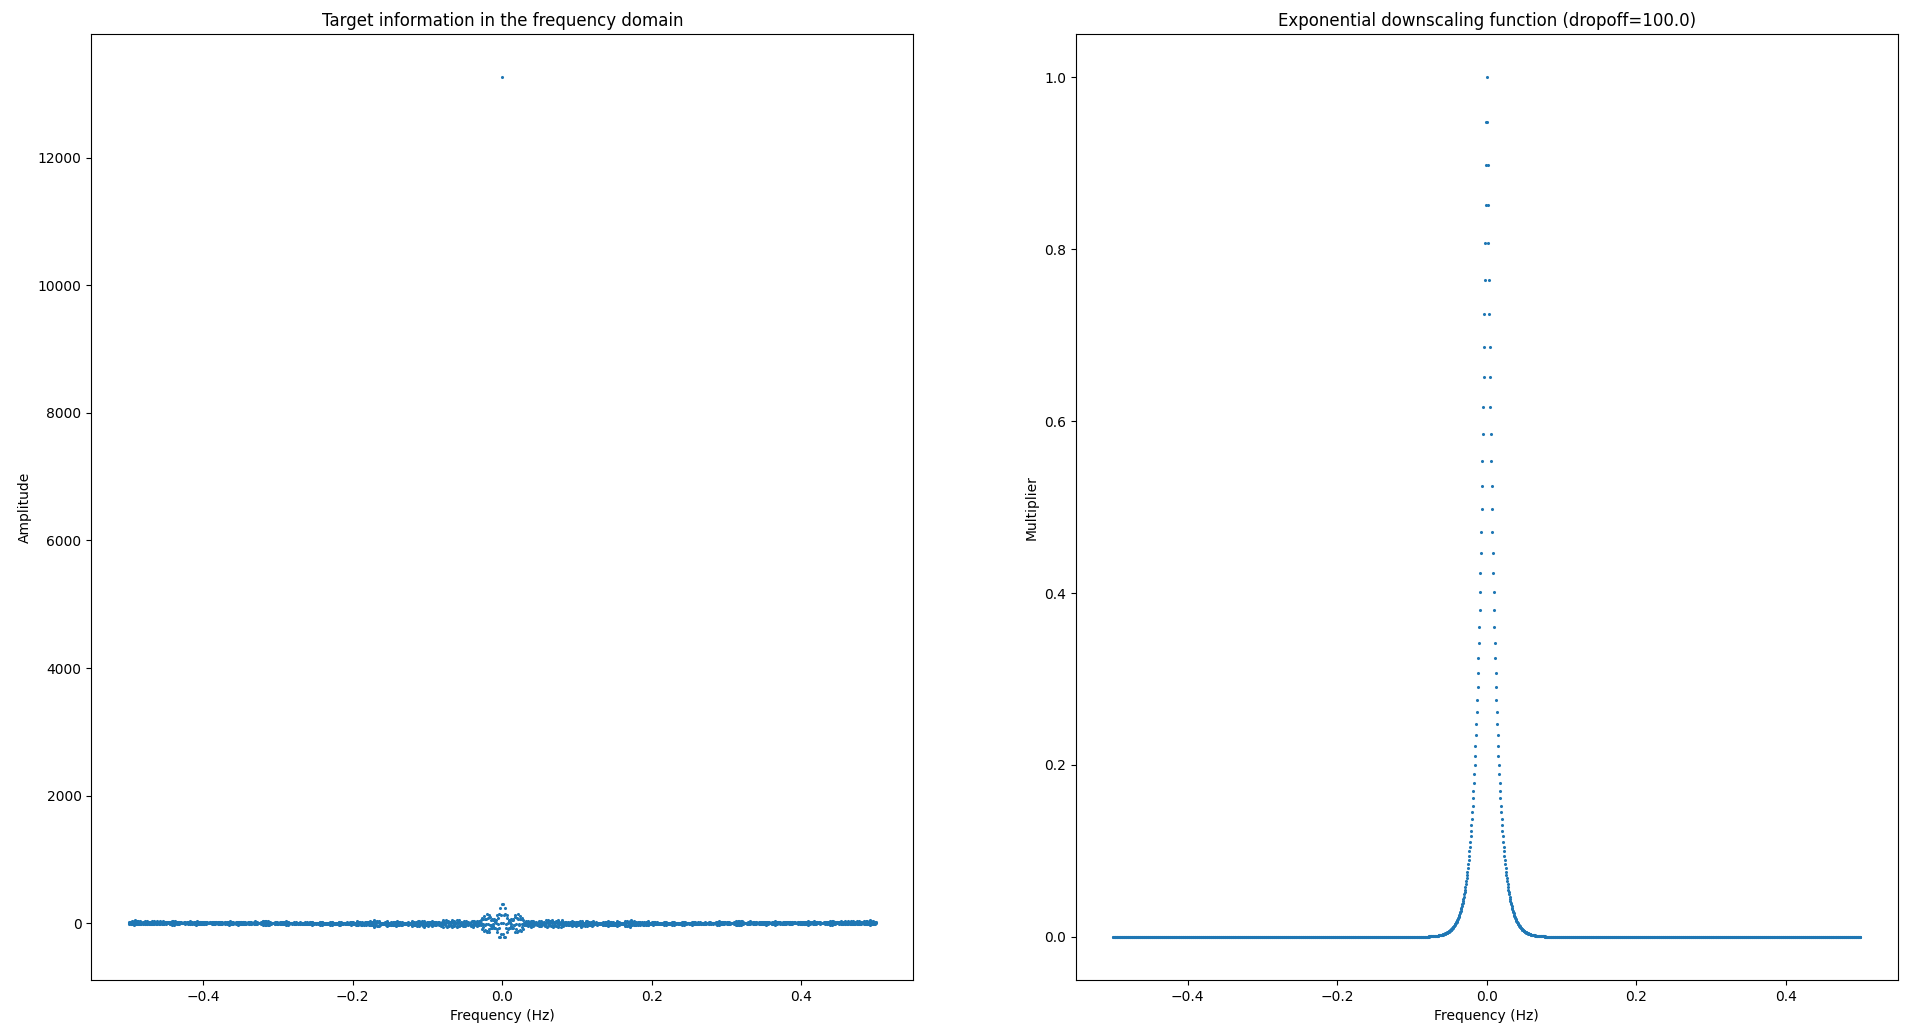
\includegraphics[width=0.95\textwidth]{./images/low_pass_filter.png}
    \caption{Example of the frequencies composing the compressed information of target \textit{all\_languages.txt} trained on the Greek reference, with default \texttt{lang} model parameters. The exponential downscaling function applied to the frequencies is also shown on the right plot.}
    \label{fig:low_pass_filter}
\end{figure}

\begin{figure}
    \centering
    \begin{subfigure}[b]{0.4\textwidth}
        \centering
        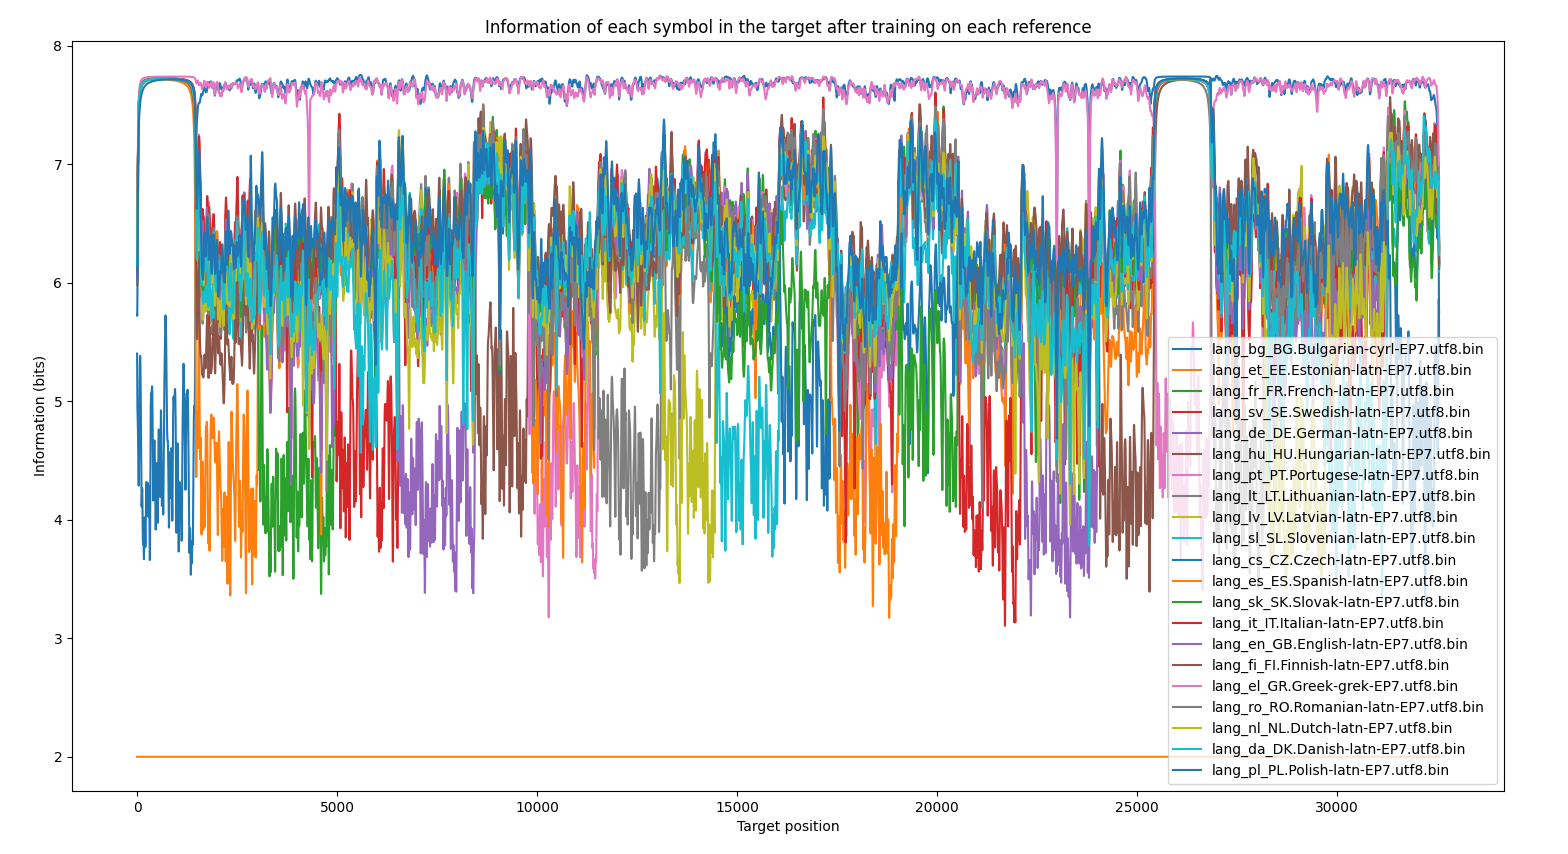
\includegraphics[width=\textwidth]{./images/no_freq_dropoff.png}
        \caption{No low-pass filter}
        \label{fig:no_freq_dropoff}
    \end{subfigure}
    \hfill
    \begin{subfigure}[b]{0.4\textwidth}
        \centering
        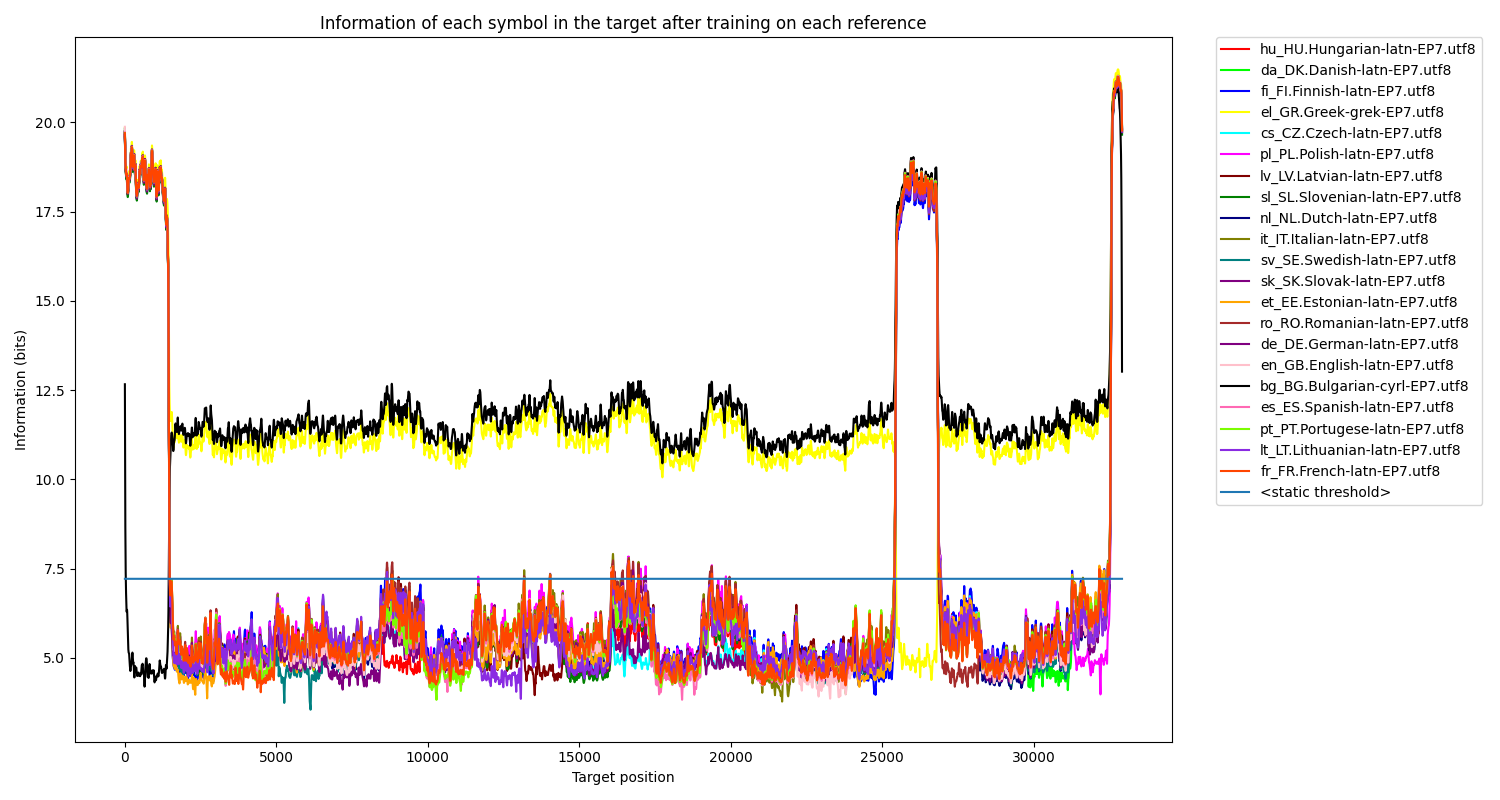
\includegraphics[width=\textwidth]{./images/freq_dropoff.png}
        \caption{Low-pass filter with frequency dropoff equal to $100.0$}
        \label{fig:freq_dropoff}
    \end{subfigure}
    \caption{Effect of the low-pass filter on the reported information at each step in \textit{all\_languages.txt}.}
    \label{fig:low_pass_filter_res}
\end{figure}

With the matrix $M$ representing the information at each step for every reference, we determine for each column, i.e. position in the target text, which row provides the minimum amount of information, that is which reference compressed the target symbol the best.
However, we don't consider all kinds of minimum values.
Since for \texttt{locate\_lang} we want to identify sections of text that we deem unknown, i.e. they likely aren't related to any of the references, then we have to consider some kind of thresholds that the minimum values have to surpass to be truly accepted.

For this we considered two thresholds, acting simultaneously:
\begin{itemize}
    \item minimum threshold: the absolute minimum value should not be larger than a given fraction of the second minimum. This threshold was implemented to disregard sections where there is confusion between more than two references. This idea is similar to the \textit{confidence} metric calculated for \texttt{find\_lang} in section \ref{subsec:methodology_find_lang}.
    \item static threshold: the absolute minimum value should not be larger than a given static threshold in bits. With this threshold, we disregard sections of text where the compression was not sufficient enough to consider that a reference truly represented the target language.
    This threshold is defined in terms of the cardinality of the target alphabet.
    More precisely, the static threshold $S$ in bits is given by the formula:

    \begin{equation}
        \label{eq:locate_lang_static_threshold}
        S = \frac{\log_2 |\Sigma|}{\gamma},
    \end{equation}

    where $\Sigma$ is the target alphabet and $\gamma$ is a real positive value.
    This way, we define the static threshold as a fraction of a baseline compression, in which the reported probability distribution at each step is a uniform distribution with each symbol having $\log_2 |\Sigma|$ bits of information.
    As such, if we set for instance $\gamma = 1$, then the threshold would be extremely forgiving, since as long as a minimal amount of compression is performed the references are considered.
    However, as $\gamma$ increases, the threshold becomes more demanding, and requires the copy model to perform well enough to fall under the threshold.
    We set $\gamma$ to a value that we consider appropriate enough for our model's performance, such that if when faced with an unkown language the model's performance should be closer to a uniform distribution and above this static threshold.
\end{itemize}

In the end, the following processing arguments are accepted:
\begin{itemize}
    \item \texttt{minimum-threshold}: fraction of the second minimum below which the absolute minimum has to be so that it is considered.
    \item \texttt{static-threshold}: denominator $\gamma$ that defines the static threshold in terms of the target alphabet's cardinality.
    \item \texttt{frequency-filter}: the frequency dropoff $\beta$ of the low-pass filter.
    \item \texttt{fill-unknown}: make an effort to consider unknown language segments as being of one of the previously identified languages, using forward and backward filling.
    \item \texttt{labeled-output}: print the target text, with segments colored depending on the identified language.
    \item \texttt{plot}: plot the entire matrix $M$ after applying the low pass filter, along with the static threshold.
    \item \texttt{save-result}: save the plot of matrix $M$ to the specified file instead of showing it (only relevant if \texttt{plot} was passed).
\end{itemize}

\section{Results}
\label{sec:results}

To test the performance of the model and the scripts implemented in this assignment, we used a set of reference texts covering 20 different languages,
these being: Bulgarian, Czech, Danish, German, Greek, English, Spanish, Estonian, Finnish, French, Hungarian, Italian, Lithuanian, Latvian, Dutch, Polish, Portuguese, Romanian, Slovak, Slovenian and Swedish.
These reference texts were obtained from the Language-Aware String Extractor Files repository \cite{references:source}.

For the target texts, we used a set of texts in the same languages as the reference texts, plus a Chinese text, but with different content, which were mainly used to test the \texttt{find\_lang} script.
And finally, to test the \texttt{locate\_lang} script, we used the following target files:

\begin{itemize}
    \item \textit{all\_languages.txt}: concatenation of the previous target files used for the \texttt{find\_lang} script, including the Chinese language at the end.
    \item \textit{all\_languages\_random.txt}: variation of \textit{all\_languages.txt} with the rows shuffled.
    \item \textit{dog.txt}: concatenation of small sentences and paragraphs of Wikipedia's ``Dog'' page in different languages \cite{wiki:dog}. This does not cover all the reference languages, but includes Chinese, and was mainly conceived to contrast \textit{all\_languages.txt} in that each language segment is relatively small, and so language transitions are performed more often.
\end{itemize}

The model's classification accuracy was measured for both the \texttt{find\_lang} and \texttt{locate\_lang} scripts, on the texts \textit{all\_languages.txt} and \textit{dog.txt}, for which we had the correct classification result.
These two targets were used additionally to check whether the length of each segment in the target text influences the model's clasification performance, where \textit{dog.txt} has smaller language segments than \textit{all\_languages.txt}.

\subsection{Find lang}
\label{subsec:results_find_lang}

To obtain the accuracy of the \texttt{find\_lang} script, we used the individual language texts and compared the result of the script with the actual language of the text.
Two runs were performed for each language file, one which executed the \texttt{lang} model using its default parameters, such as using a frequency base distribution,
and another one which used the finite-context model, instead of the other two options for probability distributions, along with the other default parameters.

For the first run, with default parameters, the script always correctly identified the language of the text, with an accuracy of 1.
\begin{equation}
    \label{eq:find_lang_default_accuracy}
    Accuracy = \frac{correct}{total} = \frac{20}{20} = 1
\end{equation}

For the second run, with the finite-context model, the script also correctly identified the language for all the texts used, with an accuracy of 1.
\begin{equation}
    \label{eq:find_lang_finite_context_accuracy}
    Accuracy = \frac{correct}{total} = \frac{20}{20} = 1
\end{equation}

To differentiate between the two approaches, we compared the confidence value given by equation \ref{eq:find_lang_confidence} presented in section \ref{subsec:methodology_find_lang}

Tables \ref{tab:find_lang_default_confidence} and \ref{tab:find_lang_finite_context_confidence} show the confidence results of the \texttt{find\_lang} script for the default parameters and the finite-context model, respectively.

\begin{table}
    \centering
    \begin{tabular}{|c|c|}
        \hline
        Language & Confidence \\
        \hline
        Bulgarian & 99.2\% \\
        Czech & 59.2\% \\
        Danish & 58.2\% \\
        German & 60.6\% \\
        Greek & 98.9\% \\
        English & 50.5\% \\
        Spanish & 46.4\% \\
        Estonian & 53.5\% \\
        Finnish & 41.2\% \\
        French & 45.8\% \\
        Hungarian & 67.1\% \\
        Italian & 45.1\% \\
        Lithuanian & 64.7\% \\
        Latvian & 74.8\% \\
        Dutch & 35.9\% \\
        Polish & 72.2\% \\
        Portuguese & 44.7\% \\
        Romanian & 74.6\% \\
        Slovak & 36.1\% \\
        Slovenian & 30.2\% \\
        Swedish & 59.8\% \\
        \hline
    \end{tabular}
    \caption{Confidence results for the \texttt{find\_lang} script with default parameters}
    \label{tab:find_lang_default_confidence}
\end{table}

\begin{table}
    \centering
    \begin{tabular}{|c|c|}
        \hline
        Language & Confidence \\
        \hline
        Bulgarian & 93.1\% \\
        Czech & 77.3\% \\
        Danish & 85.5\% \\
        German & 92.1\% \\
        Greek & 93.9\% \\
        English & 92.3\% \\
        Spanish & 86.4\% \\
        Estonian & 90.4\% \\
        Finnish & 89.7\% \\
        French & 91.7\% \\
        Hungarian & 92.9\% \\
        Italian & 90.2\% \\
        Lithuanian & 90.4\% \\
        Latvian & 89.8\% \\
        Dutch & 91.1\% \\
        Polish & 89.4\% \\
        Portuguese & 82.7\% \\
        Romanian & 91.2\% \\
        Slovak & 77.8\% \\
        Slovenian & 86.7\% \\
        Swedish & 89.2\% \\
        \hline
    \end{tabular}
    \caption{Confidence results for the \texttt{find\_lang} script with finite-context model}
    \label{tab:find_lang_finite_context_confidence}
\end{table}

By comparing the confidence results of the two approaches, we can see that although both approaches correctly identified the language of the text,
the default parameters approach had a much lower average confidence value than the finite-context model approach, some of them being even lower than 50\%.

The reason for this is that the default parameters approach uses a frequency base distribution, which is not very good at identifying the language of a text,
because it does not take into account the order of the characters in the text, which is very important for some languages.

After comparing the confidence values, we also tested the script with a text of a language that was not in the reference files, in this case, Chinese.
Due to the fact that the script always returns a language, the way to evaluate the accuracy of the script is by checking if the returned language has a very low confidence value.

For the default parameters approach, the script returned the language as Hungarian, with a confidence value of 37.7\%, which is low, but not low enough considering the other confidence values and
the fact that chinese has a completely different alphabet than any of the other languages present in the reference files.
In contrast, the finite-context model approach returned the language as Swedish, but with a confidence value of 0.0\%, which is the lowest possible value, and the correct result
for a language that is not in the reference files.

With these results we can conclude that the probability distribution based on the finite-context model is better than the default approach and has a really good accuracy and confidence value.

\subsection{Locate lang}
\label{subsec:results_locate_lang}

For \texttt{locate\_lang}, we created plots evaluating the reported information at each position in the target files \textit{all\_languages.txt} and \textit{all\_languages\_random.txt} using different \texttt{lang} model configurations, to check the effect that each parameter has in the overall language segmentation process.
We also evaluated the classification accuracy for the target files \textit{all\_languages.txt} and \textit{dog.txt}, using different \texttt{lang} model configurations and different result processing parameters for the script itself.

Unless stated otherwise, for all plots showing the reported information at each target position, the script and \texttt{lang} model parameters are the default ones.

\subsubsection{Base probability distribution - Uniform distribution}
\label{subsubsec:results_locate_lang_uniform_distribution}

% CUNHA
By using this approach, we can see very clearly the different languages in figure \ref{fig:all_languages_p_u} of file \textit{all\_languages.txt},
because the reported information of the correct language is much lower than all the others.
But by using this approach, we have more difficulty detecting unknown languages (languages that are not in the references).
Because even if we define the static threshold at the lowest information values of all the correct languages,
it will also detect the last chunk of text as French, which is wrong, as the last chunk of text in the file is Chinese.

For \textit{all\_languages\_random.txt}, we can distinguish the languages in figure \ref{fig:all_languages_random_p_u}.
We can see the valleys very clearly and infer the language using that information.
The same difficulty is seen in this figure: we can't define a static threshold without affecting some of the real languages.
(We can't draw a horizontal line that is above all the reference languages and under the Chinese one.)

\begin{figure}
    \centering
    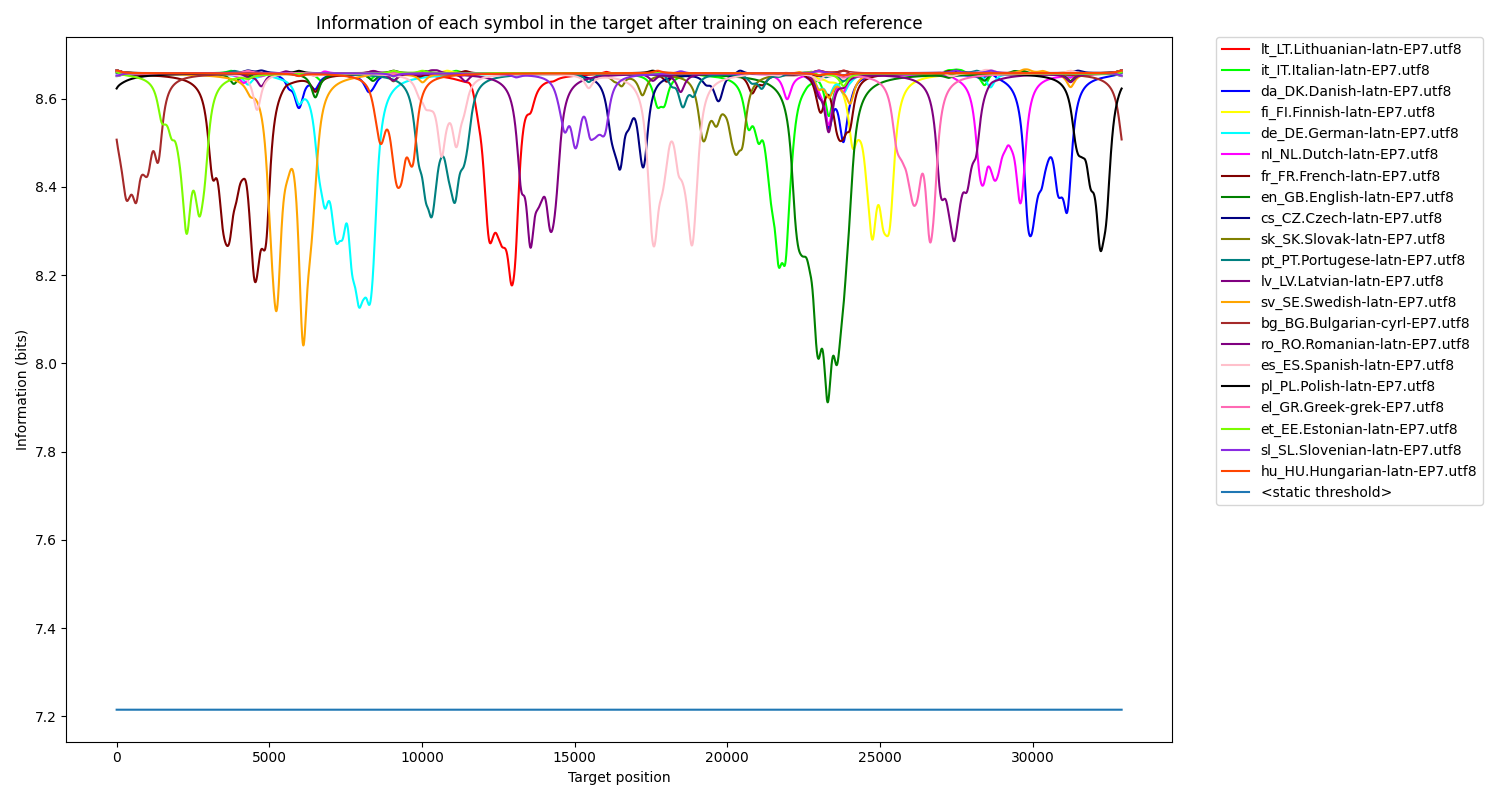
\includegraphics[width=0.95\textwidth]{../results/all_languages/-p_u.png}
    \caption{Information at each step for each language for \textit{all\_languages.txt}, uniform distribution.}
    \label{fig:all_languages_p_u}
\end{figure}

\begin{figure}
    \centering
    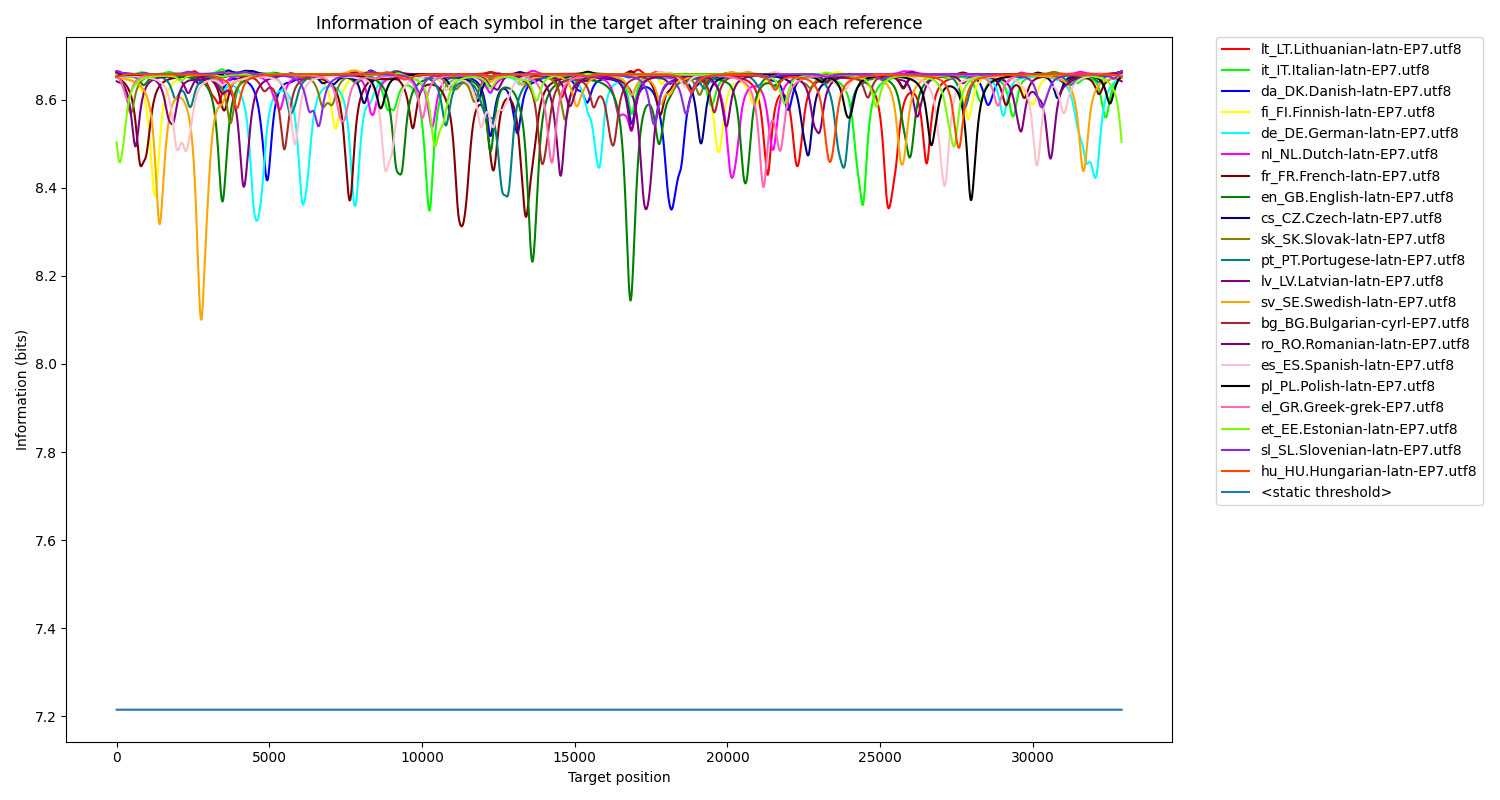
\includegraphics[width=0.95\textwidth]{../results/all_languages_random/-p_u.png}
    \caption{Information at each step for each language for \textit{all\_languages\_random.txt}, uniform distribution.}
    \label{fig:all_languages_random_p_u}
\end{figure}

\subsubsection{Base probability distribution - Frequency distribution}
\label{subsubsec:results_locate_lang_frequency_distribution}

Using this approach, we can see the different languages in figure \ref{fig:all_languages_p_f} of file \textit{all\_languages.txt}, although it produces a very different plot
compared to the uniform distribution approach.

It is still possible to distinguish the languages in figure \ref{fig:all_languages_random_p_f} of file \textit{all\_languages\_random.txt}, but it is harder to do so,
and another difference is between Bulgarian and Greek languages to the other languages. These have a much higher reported information than the others, due to the fact that these
languages use a completely different alphabet than the others.

A downside of this approach is that the static threshold line becomes relatively higher, which means most of the languages will pass the threshold, even in their peak information values,
at least in the case of the \textit{all\_languages.txt} file. For the \textit{all\_languages\_random.txt} file, the peaks are higher due to each line in the file being a random language, incurring in many more prediction fails.

Still, even with this downside, the script still manages to correctly identify the language of the sections, albeit with less accuracy in the entire interval on the random file,
due to the constant change of languages.

\begin{figure}
    \centering
    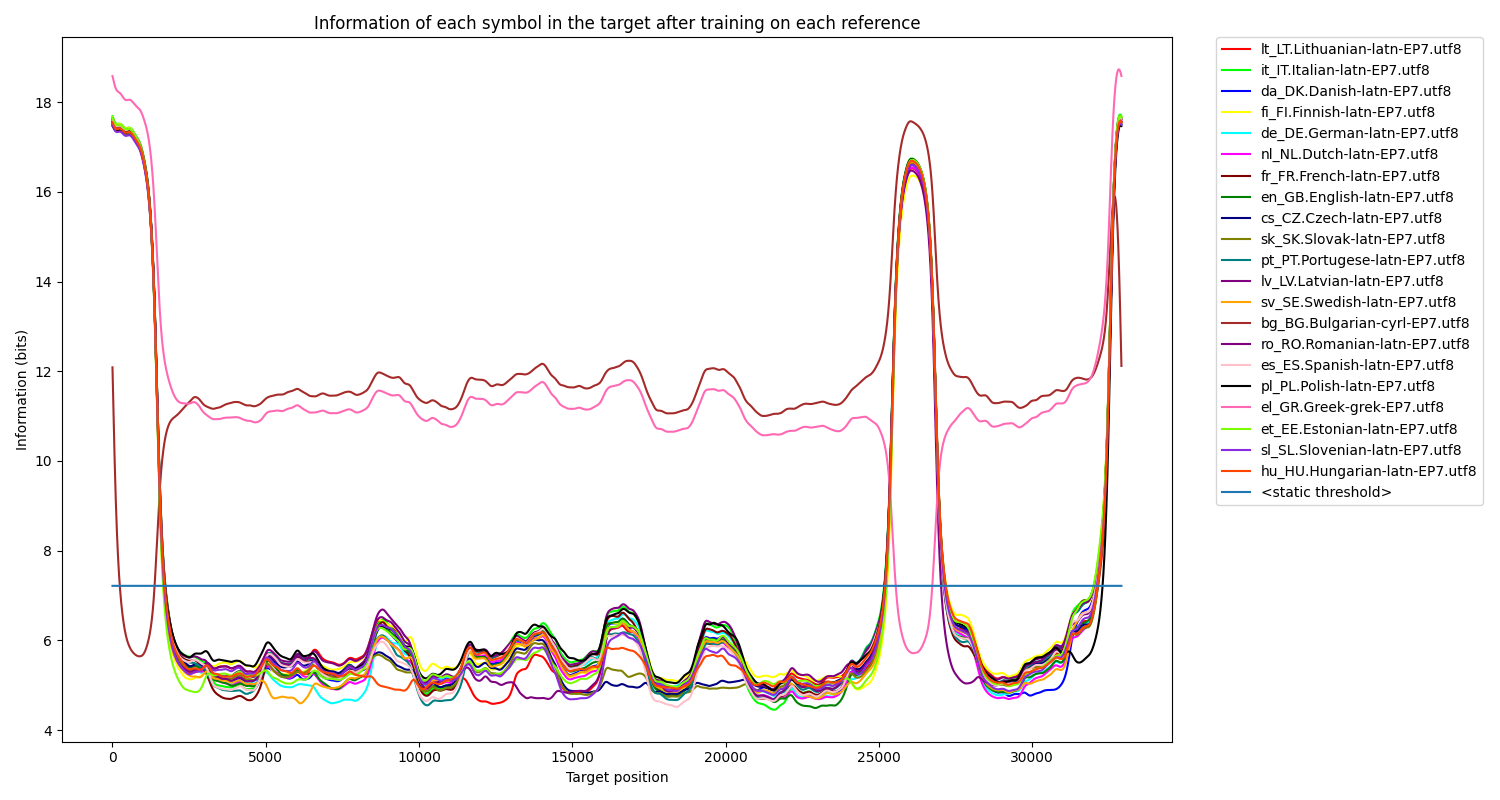
\includegraphics[width=0.95\textwidth]{../results/all_languages/-p_f.png}
    \caption{Information at each step for each language for \textit{all\_languages.txt}, frequency distribution.}
    \label{fig:all_languages_p_f}
\end{figure}

\begin{figure}
    \centering
    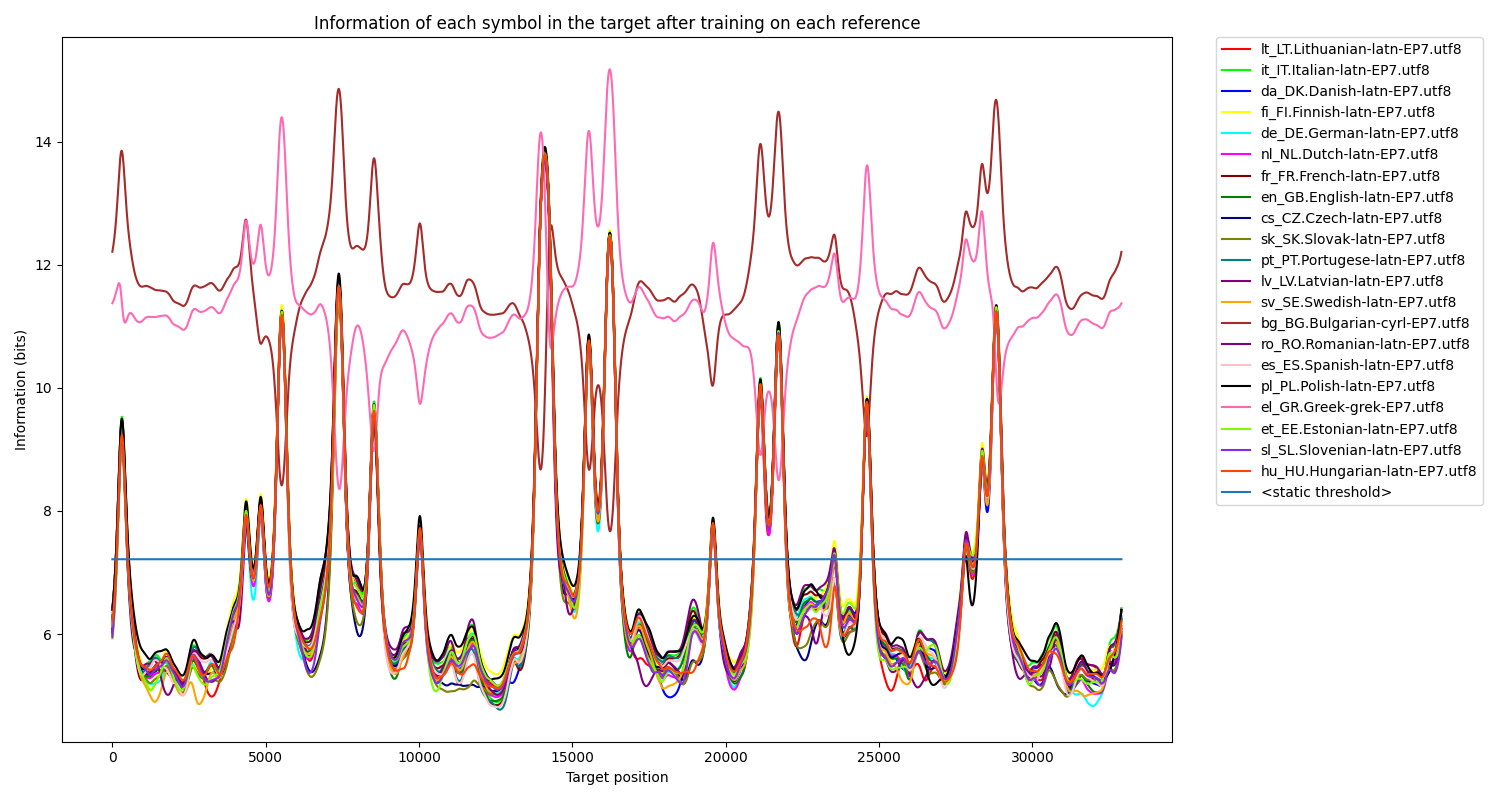
\includegraphics[width=0.95\textwidth]{../results/all_languages_random/-p_f.png}
    \caption{Information at each step for each language for \textit{all\_languages\_random.txt}, frequency distribution.}
    \label{fig:all_languages_random_p_f}
\end{figure}

\subsubsection{Base probability distribution - Finite-context model}
\label{subsubsec:results_locate_lang_first_order_fcm}

To test this approach, two sub-parameters were tested: the size of the context and the smoothing parameter used to calculate the probability distribution.

For the context size, $k_f$ was tested with 3, 6 and 9, and for the smoothing parameter, $\alpha$, the values tested were 1, 10 and 100.
The results for both files are shown in figures \ref{fig:all_languages_p_c} and \ref{fig:all_languages_random_p_c}.

By verifiying the results for the context size in figure \ref{fig:all_languages_p_c}, we can see that the finite-context model produces a much better result than the other probability distribution approaches,
because it is able to clearly distinguish the correct language (the minimum value) from the second best candidate.
When increasing $k$, this difference becomes even more clear, as seen in figures \ref{fig:all_languages_p_c:1:3} and \ref{fig:all_languages_p_c:1:6},
although increases the overall reported information per language, which makes the static threshold too low to detect the correct language in each section.

This problem can also be seen in the random file, in figure \ref{fig:all_languages_random_p_c}, where the threshold line is too low to detect the correct language in each section when the context size
becomes $6$ or $9$.
Similarly, it is also possible to verify, although not as clearly due to the random nature of the file, that the correct language becomes more clear when increasing the context size.

This is due to the threshold not being tailor made for each file, but instead being a static value, which is not ideal, although it is clearly visible what the correct language is
in each section due to the difference in information values between the correct language and the second best candidate.

Now for the smoothing parameter, $\alpha$, we can see that the results are very similar for all the values tested, as seen in figures \ref{fig:all_languages_p_c:1:3_again}, \ref{fig:all_languages_p_c:10:3},
with the biggest difference being more noticiable in the random file, in figure \ref{fig:all_languages_random_p_c:100:3}, where the static threshold line is too low to detect the correct language.
This is due to the fact that increasing the smoothing parameter increases the information value of each language, by making the probability distributions approximate a uniform distribution, which makes the threshold line too low to detect the correct language in each section.

Through these results, the best value for $\alpha$ was $10$ and for the context size was $3$, because these helped to distinguish the correct language from the second best candidate, while not increasing the overall reported information too much to make the threshold line relatively low.

\begin{figure}
    \begin{subfigure}[b]{0.3\textwidth}
        \begin{center}
            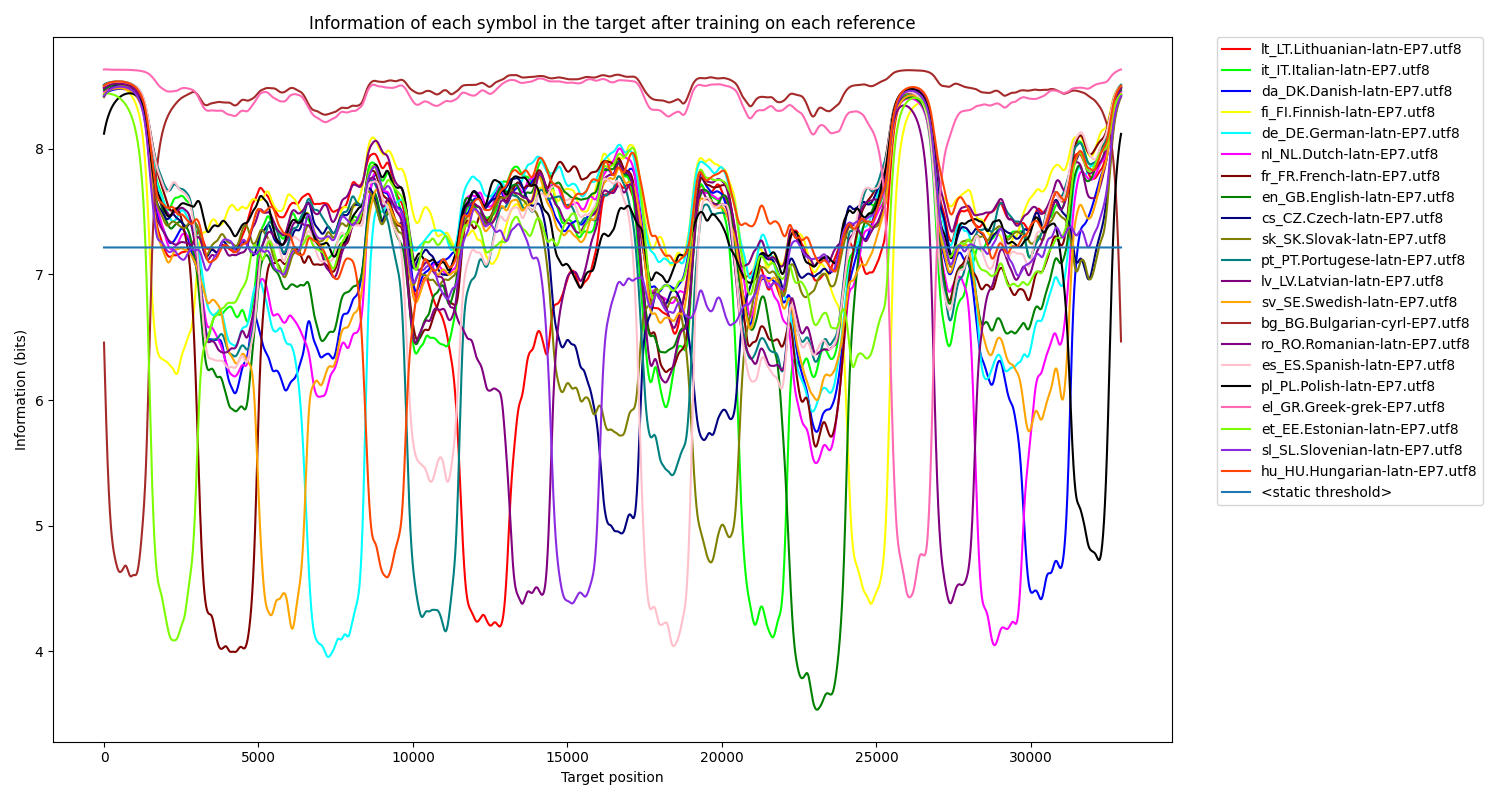
\includegraphics[width=1.0\linewidth]{../results/all_languages/-p_c:1:3.png}
        \end{center}
        \caption{$k = 3$}
        \label{fig:all_languages_p_c:1:3}
    \end{subfigure}
    \hfill
    \begin{subfigure}[b]{0.3\textwidth}
        \begin{center}
            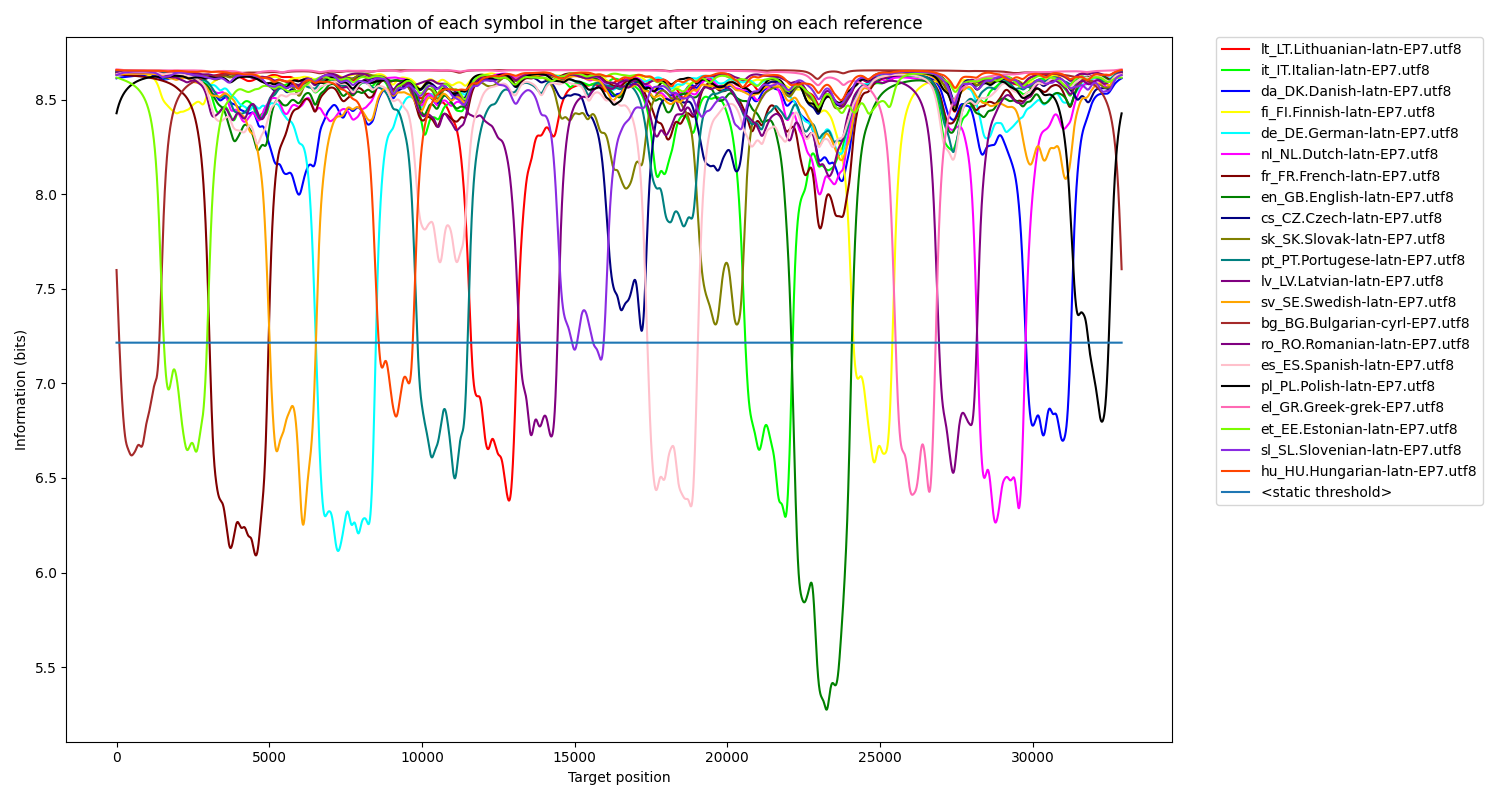
\includegraphics[width=1.0\linewidth]{../results/all_languages/-p_c:1:6.png}
        \end{center}
        \caption{$k = 6$}
        \label{fig:all_languages_p_c:1:6}
    \end{subfigure}
    \hfill
    \begin{subfigure}[b]{0.3\textwidth}
        \begin{center}
            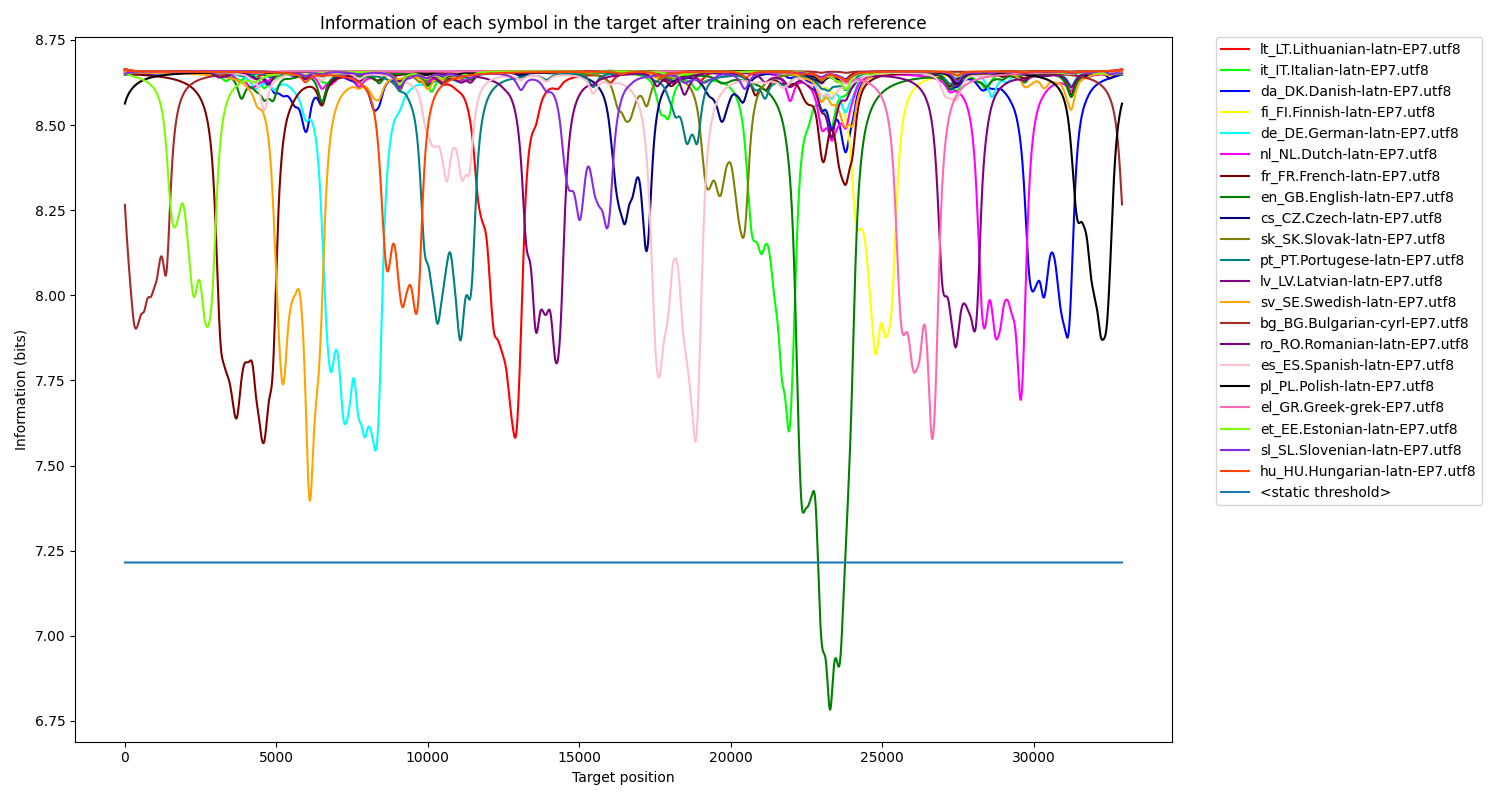
\includegraphics[width=1.0\linewidth]{../results/all_languages/-p_c:1:9.png}
        \end{center}
        \caption{$k = 9$}
        \label{fig:all_languages_p_c:1:9}
    \end{subfigure}
    
    \caption{Information at each step for each language for \textit{all\_languages.txt}, finite-context model by changing $k$.}
    \label{fig:all_languages_p_c}
\end{figure}

\begin{figure}
    \begin{subfigure}[b]{0.3\textwidth}
        \begin{center}
            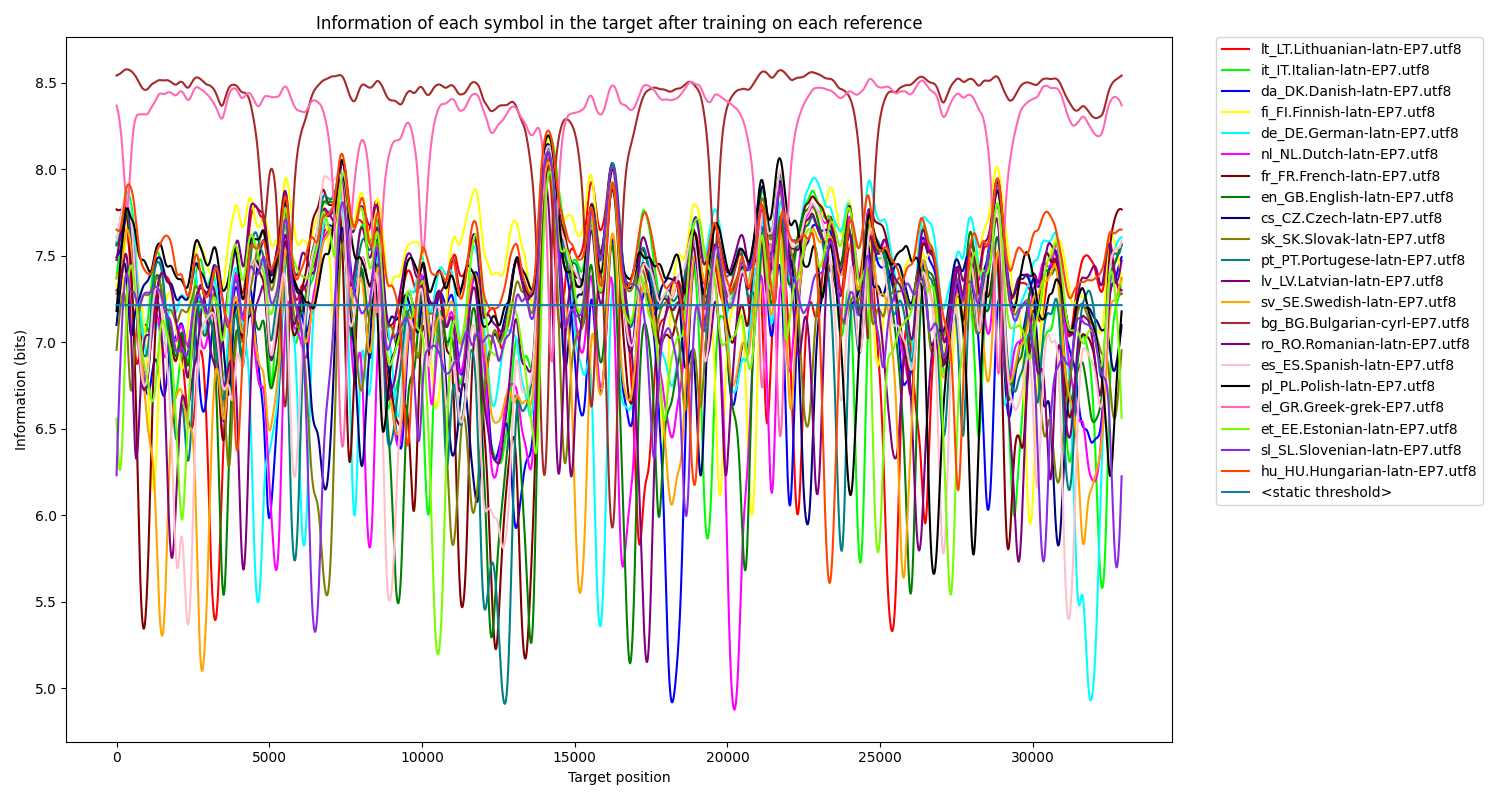
\includegraphics[width=1.0\linewidth]{../results/all_languages_random/-p_c:1:3.png}
        \end{center}
        \caption{$k = 3$}
        \label{fig:all_languages_random_p_c:1:3}
    \end{subfigure}
    \hfill
    \begin{subfigure}[b]{0.3\textwidth}
        \begin{center}
            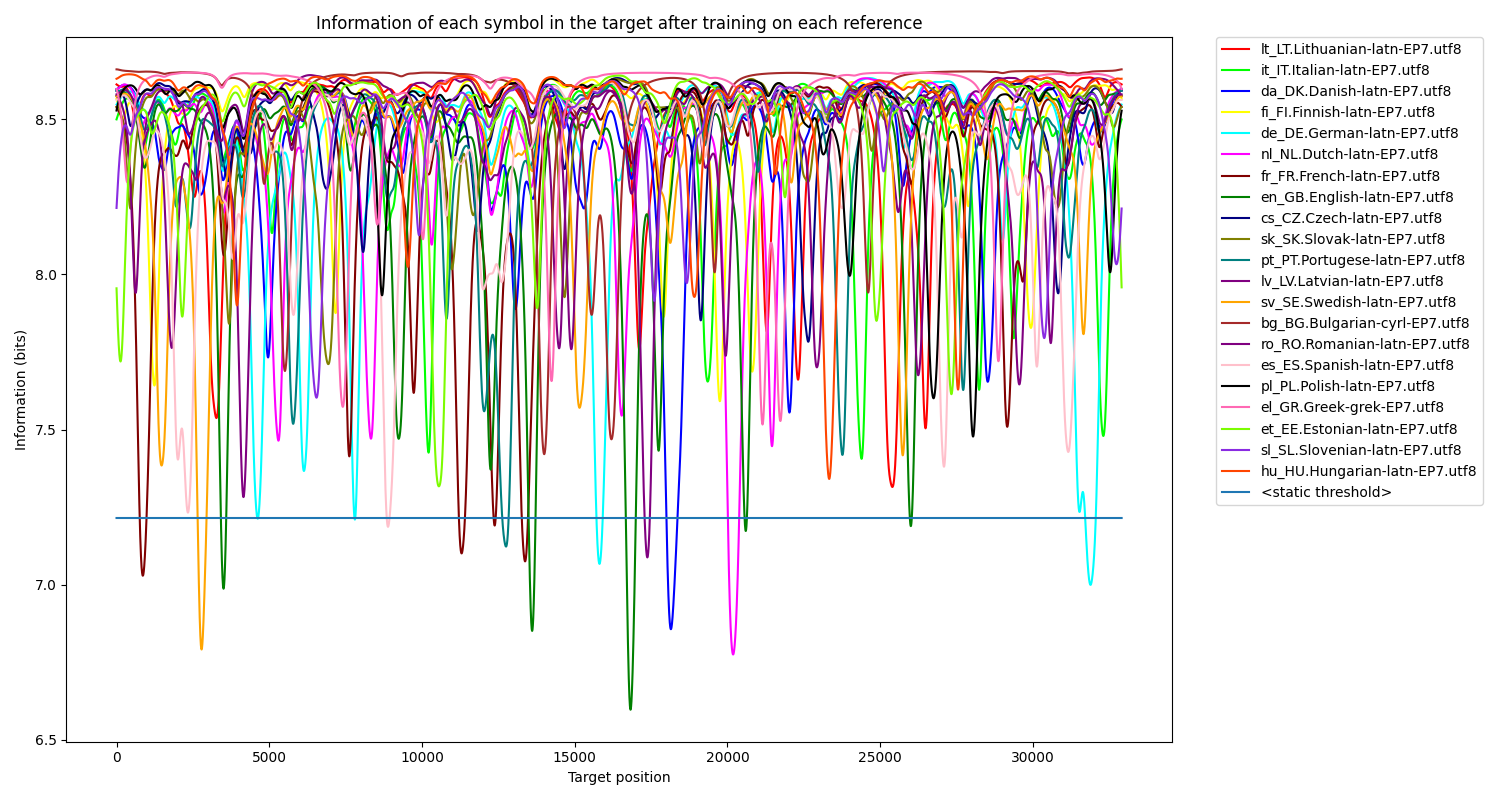
\includegraphics[width=1.0\linewidth]{../results/all_languages_random/-p_c:1:6.png}
        \end{center}
        \caption{$k = 6$}
        \label{fig:all_languages_random_p_c:1:6}
    \end{subfigure}
    \hfill
    \begin{subfigure}[b]{0.3\textwidth}
        \begin{center}
            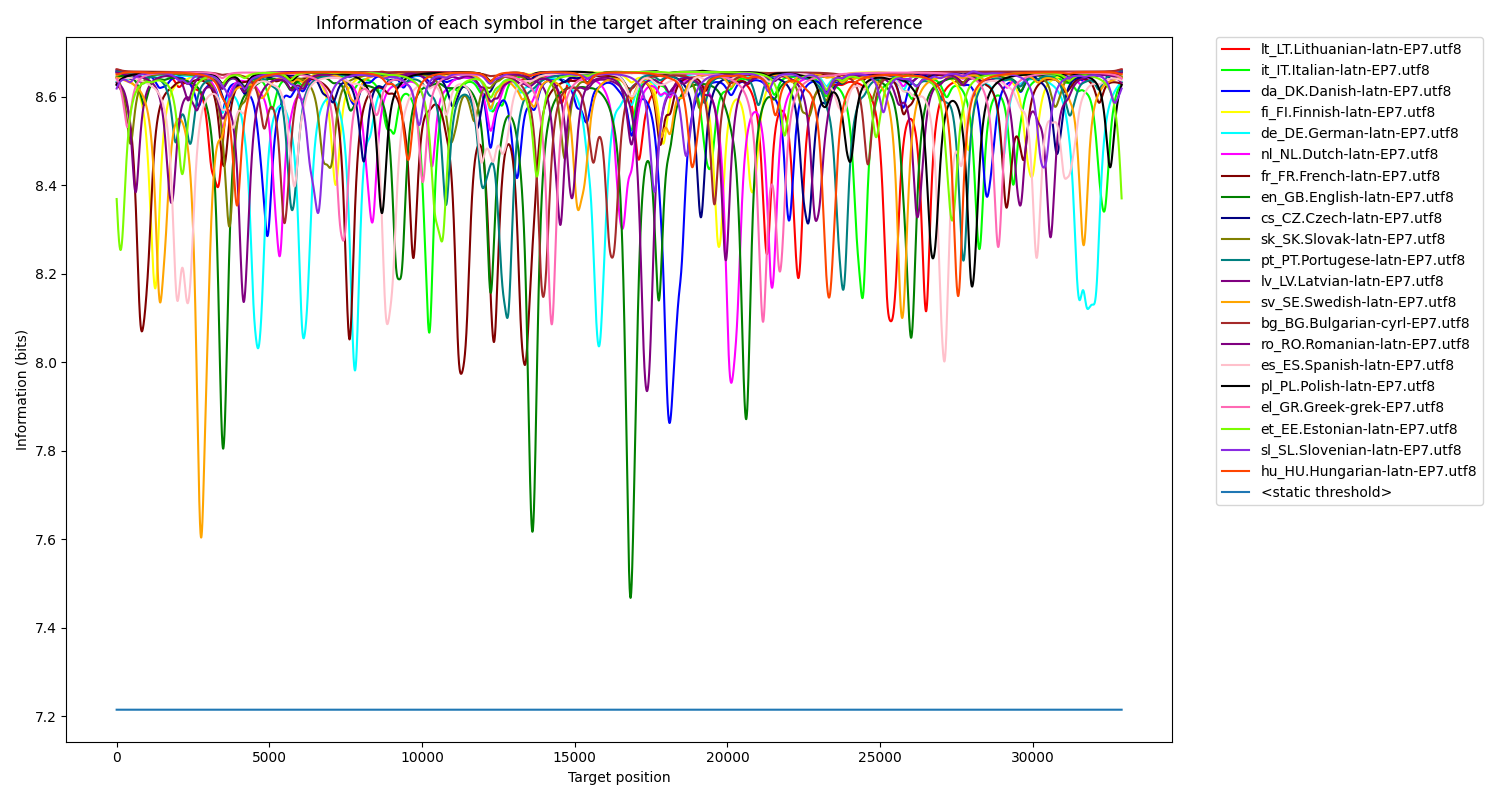
\includegraphics[width=1.0\linewidth]{../results/all_languages_random/-p_c:1:9.png}
        \end{center}
        \caption{$k = 9$}
        \label{fig:all_languages_random_p_c:1:9}
    \end{subfigure}
    
    \caption{Information at each step for each language for \textit{all\_languages\_random.txt}, finite-context model by changing $k$.}
    \label{fig:all_languages_random_p_c}
\end{figure}


\begin{figure}
    \begin{subfigure}[b]{0.3\textwidth}
        \begin{center}
            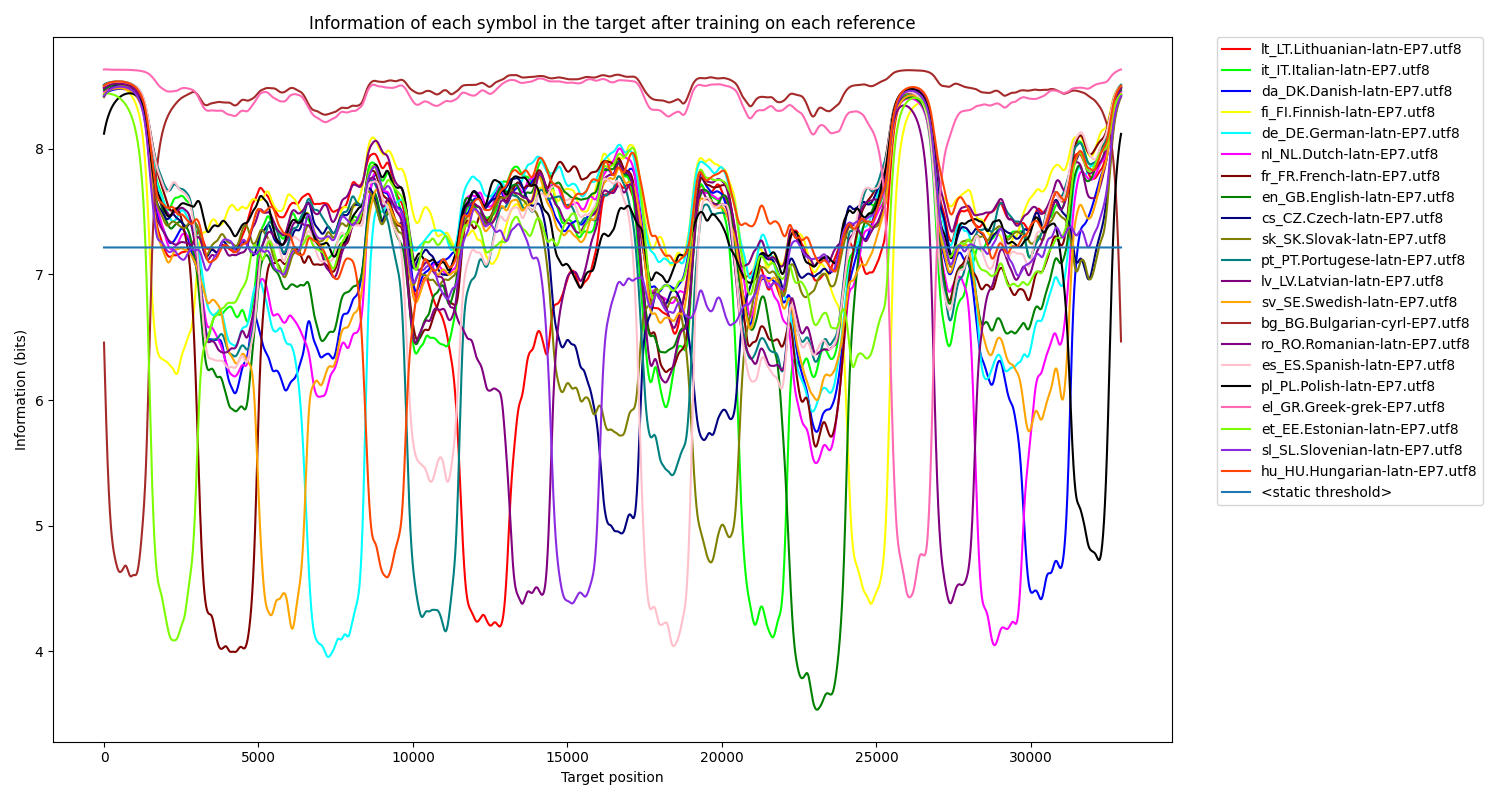
\includegraphics[width=1.0\linewidth]{../results/all_languages/-p_c:1:3.png}
        \end{center}
        \caption{$\alpha = 1$}
        \label{fig:all_languages_p_c:1:3_again}
    \end{subfigure}
    \hfill
    \begin{subfigure}[b]{0.3\textwidth}
        \begin{center}
            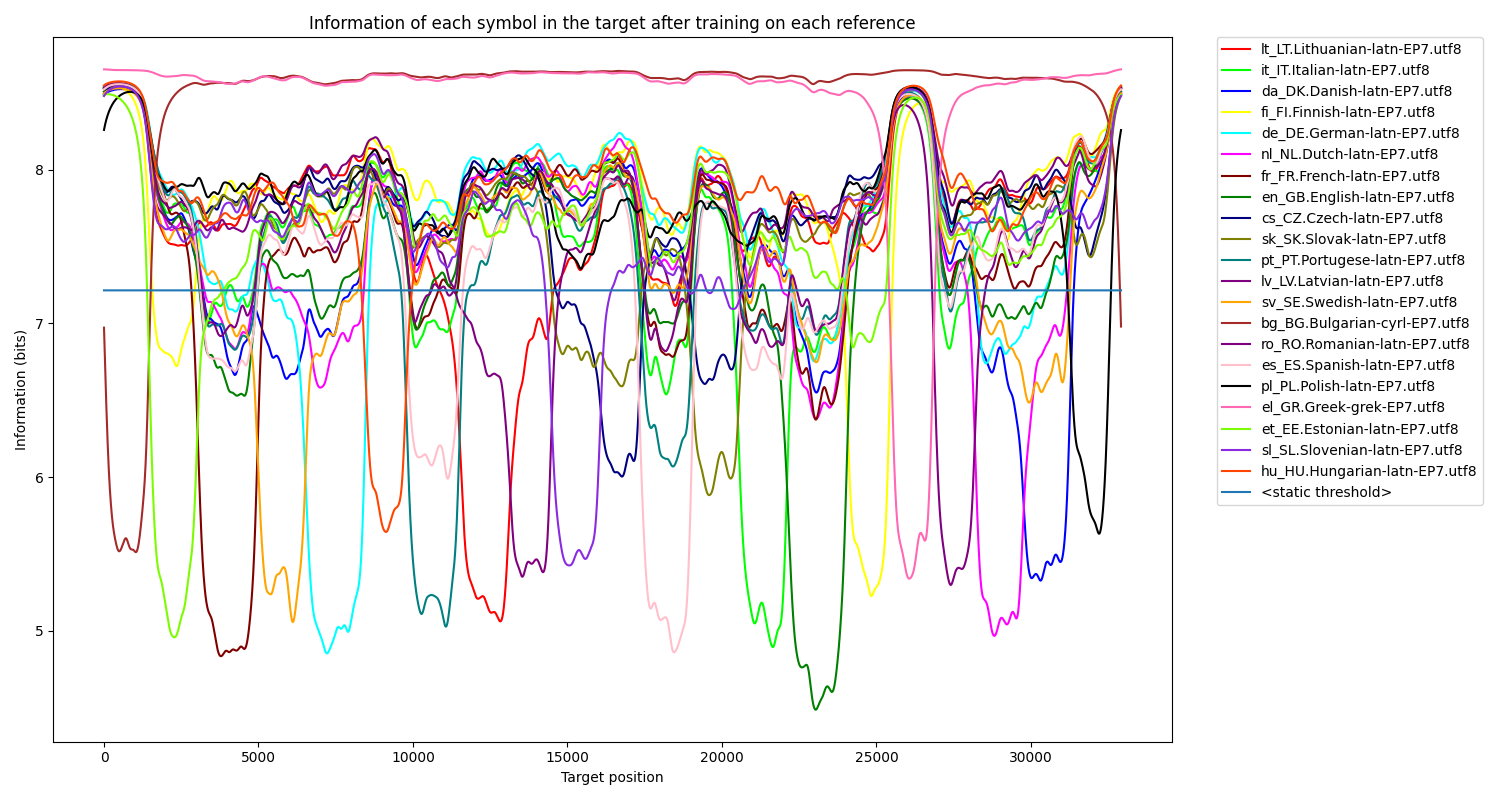
\includegraphics[width=1.0\linewidth]{../results/all_languages/-p_c:10:3.png}
        \end{center}
        \caption{$\alpha = 10$}
        \label{fig:all_languages_p_c:10:3}
    \end{subfigure}
    \hfill
    \begin{subfigure}[b]{0.3\textwidth}
        \begin{center}
            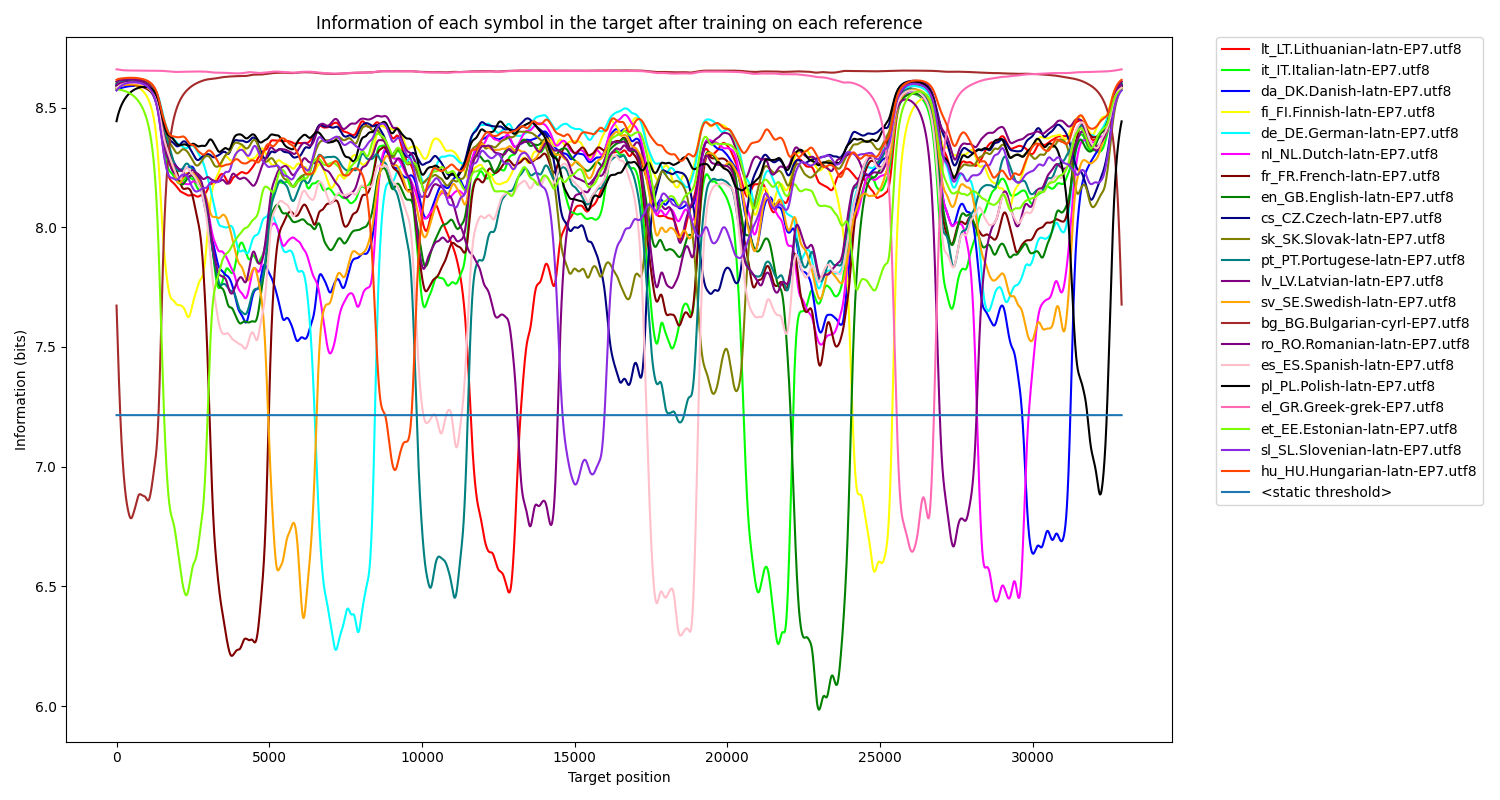
\includegraphics[width=1.0\linewidth]{../results/all_languages/-p_c:100:3.png}
        \end{center}
        \caption{$\alpha = 100$}
        \label{fig:all_languages_p_c:100:3}
    \end{subfigure}
    
    \caption{Information at each step for each language for \textit{all\_languages.txt}, finite-context model by changing $\alpha$.}
    \label{fig:all_languages_p_c:alpha}
\end{figure}

\begin{figure}
    \begin{subfigure}[b]{0.3\textwidth}
        \begin{center}
            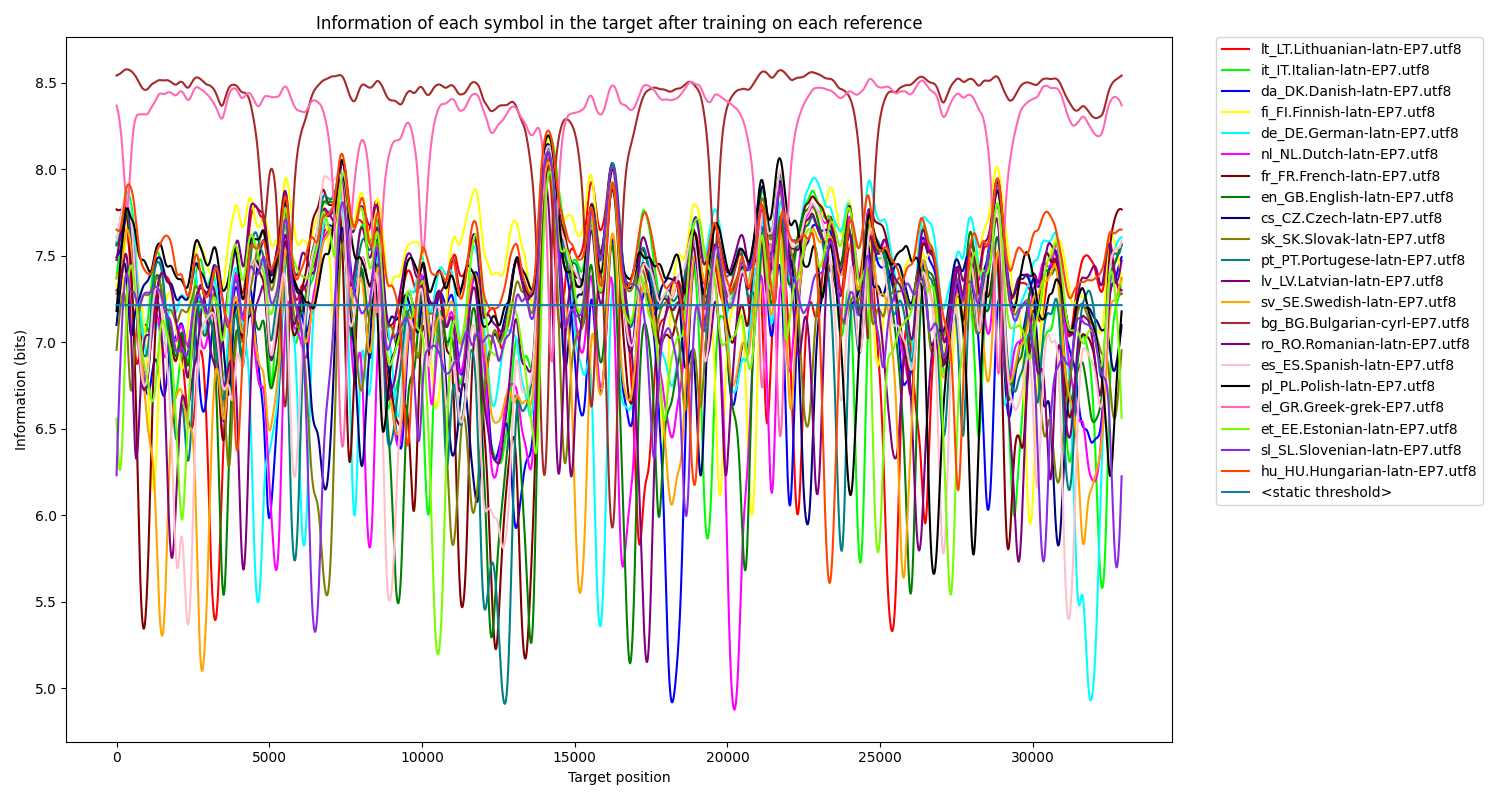
\includegraphics[width=1.0\linewidth]{../results/all_languages_random/-p_c:1:3.png}
        \end{center}
        \caption{$\alpha = 1$}
        \label{fig:all_languages_random_p_c:1:3_again}
    \end{subfigure}
    \hfill
    \begin{subfigure}[b]{0.3\textwidth}
        \begin{center}
            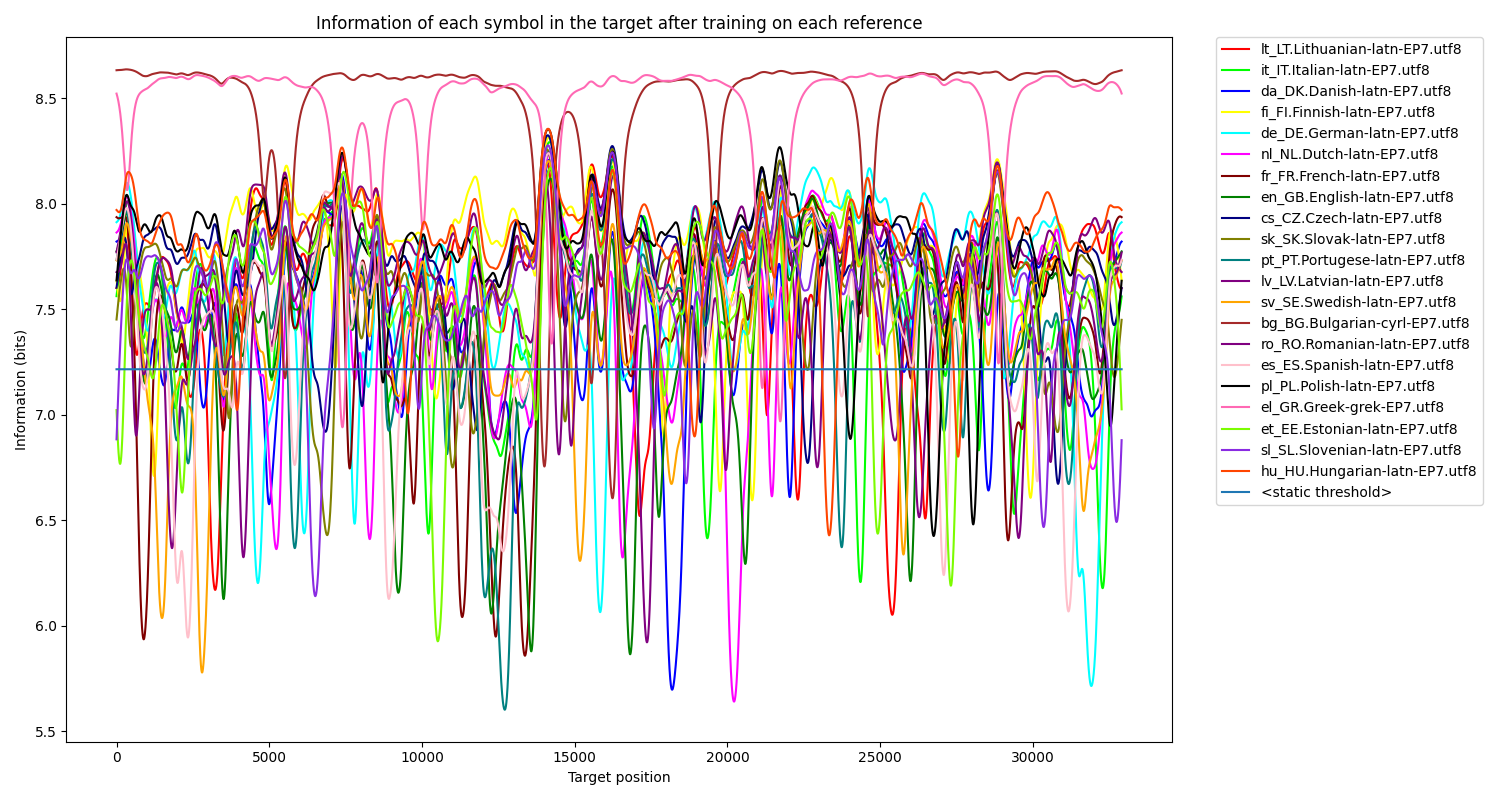
\includegraphics[width=1.0\linewidth]{../results/all_languages_random/-p_c:10:3.png}
        \end{center}
        \caption{$\alpha = 10$}
        \label{fig:all_languages_random_p_c:10:3}
    \end{subfigure}
    \hfill
    \begin{subfigure}[b]{0.3\textwidth}
        \begin{center}
            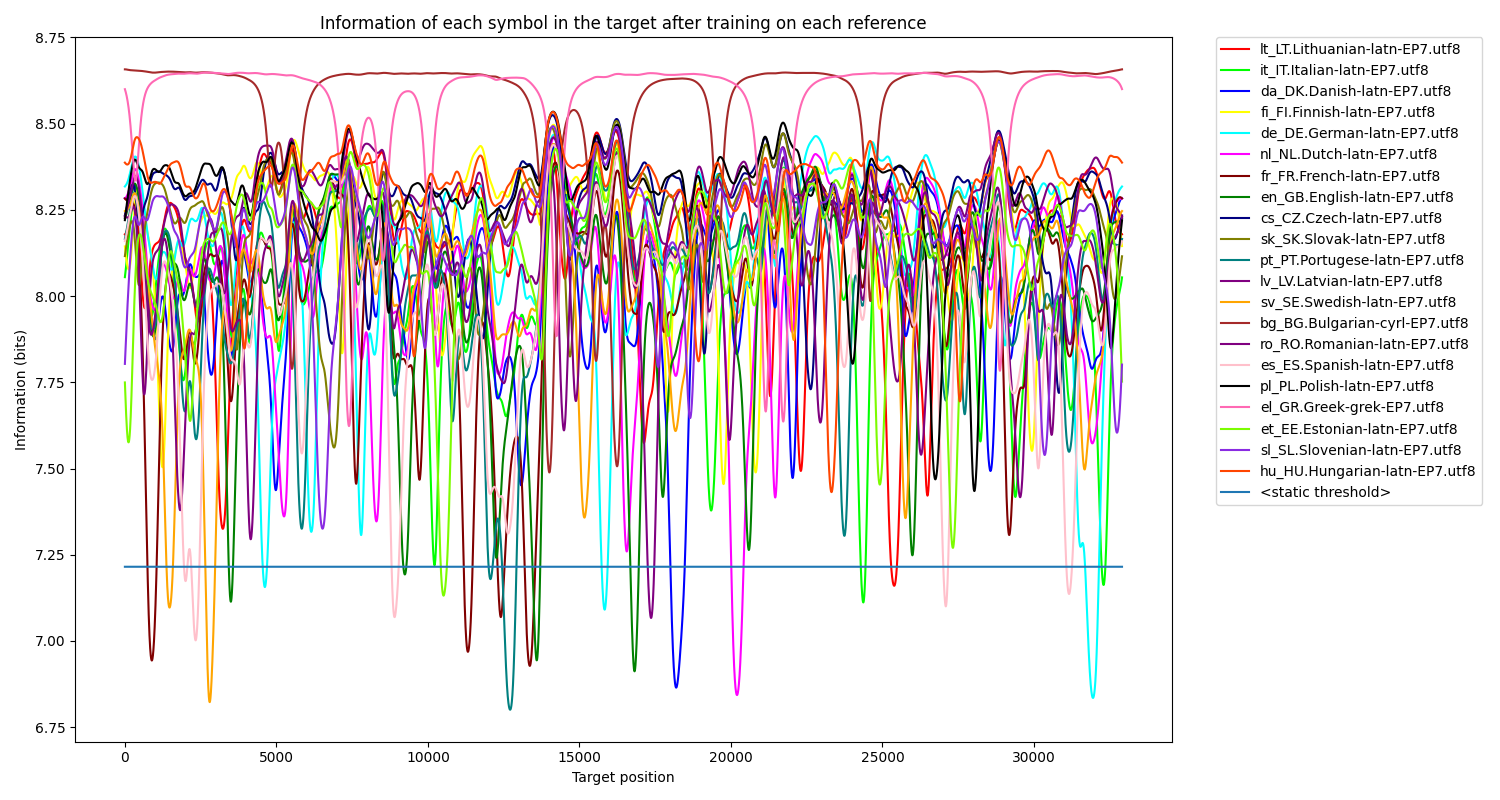
\includegraphics[width=1.0\linewidth]{../results/all_languages_random/-p_c:100:3.png}
        \end{center}
        \caption{$\alpha = 100$}
        \label{fig:all_languages_random_p_c:100:3}
    \end{subfigure}
    
    \caption{Information at each step for each language for \textit{all\_languages\_random.txt}, finite-context model by changing $\alpha$.}
    \label{fig:all_languages_random_p_c:alpha}
\end{figure}

\subsubsection{Copy pointer repositioning - Oldest pointer first}
\label{subsubsec:results_locate_lang_oldest_pointer_first}

To see the effect of the pointer repositioning, we tested the different approaches when using a frequency distribution, which was the default parameter when testing.
So these results will be mostly similar with the results shown for the frequency distribution section.

In this approach we can still distinguish the different languages, but not as clearly as some of the previous approaches.
In figure \ref{fig:all_languages_r_o} we can see that the reported information by the languages are mostly the same, excluding Greek and Bulgarian.
For the \textit{all\_languages\_random.txt} file we can see in the figure \ref{fig:all_languages_r_o}, that the same behavior is seen, but now with slightly more differences between languages.

\begin{figure}
    \centering
    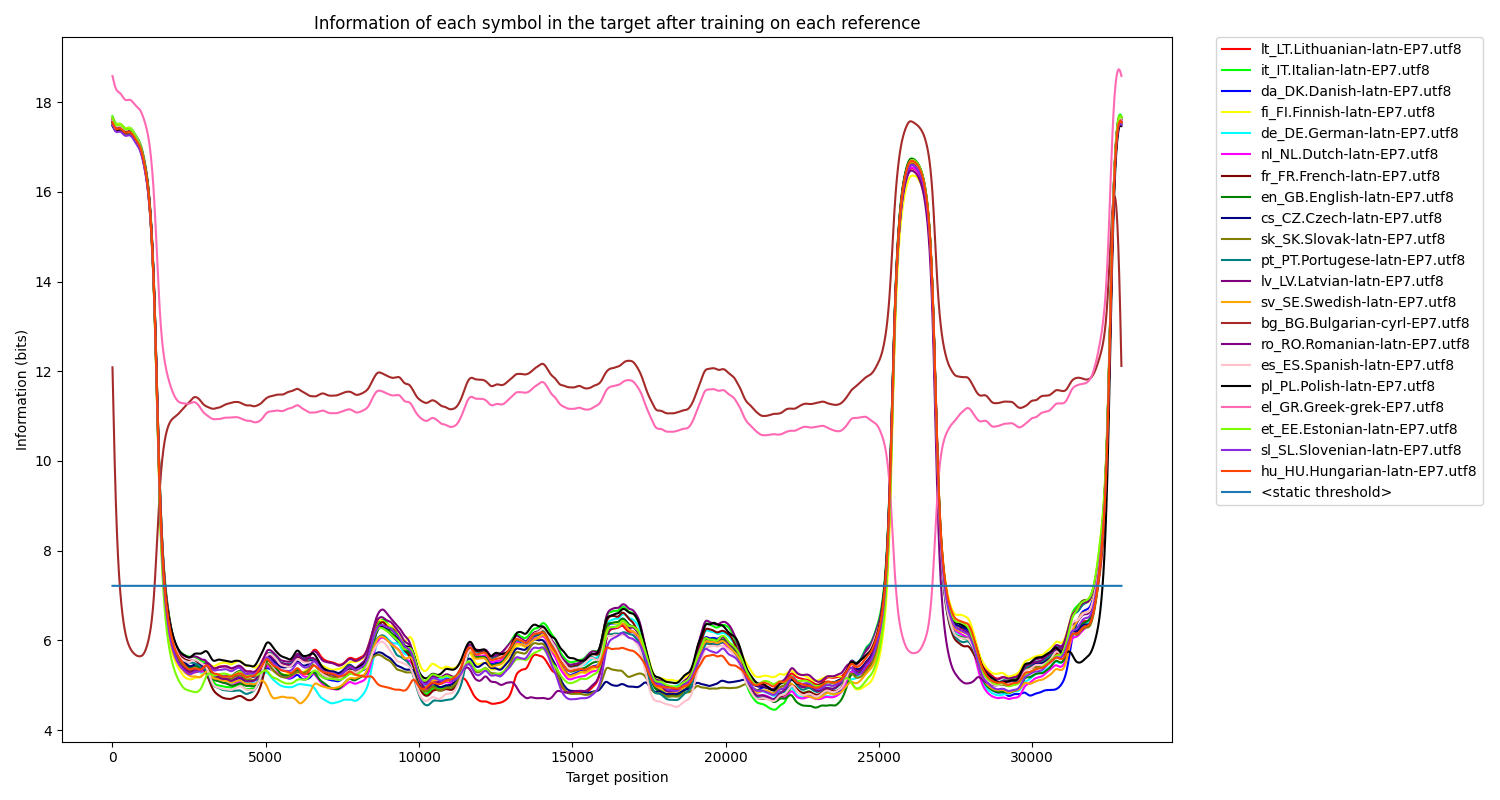
\includegraphics[width=0.95\textwidth]{../results/all_languages/-r_o.png}
    \caption{Information at each step for each language for \textit{all\_languages.txt}, oldest pointer first.}
    \label{fig:all_languages_r_o}
\end{figure}

\begin{figure}
    \centering
    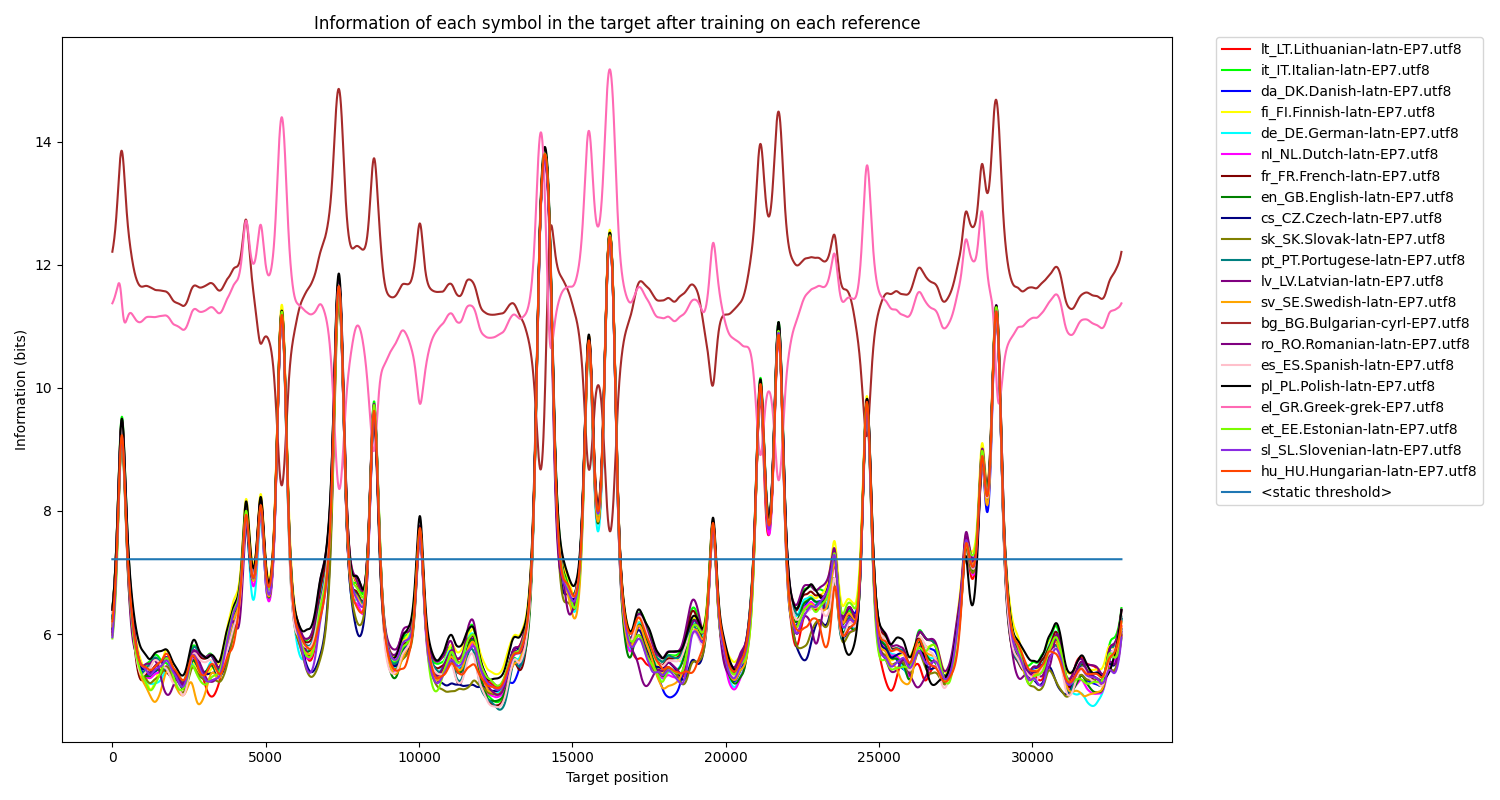
\includegraphics[width=0.95\textwidth]{../results/all_languages_random/-r_o.png}
    \caption{Information at each step for each language for \textit{all\_languages\_random.txt}, oldest pointer first.}
    \label{fig:all_languages_random_r_o}
\end{figure}

\subsubsection{Copy pointer repositioning - Newest pointer first}
\label{subsubsec:results_locate_lang_newest_pointer_first}

Like in the oldest pointer approach, we can still distinguish the different languages, using the newest pointer.
In both the \ref{fig:all_languages_r_n} and \ref{fig:all_languages_random_r_n}, we can see that the behavior is extremely similar to the oldest pointer approach.
Technically, since the reference has already been trained on and there may not be any connection between the reference and the target, e.g. there is no ``continuity'' in the message like in the first assignment where prediction and training is done at the same time on the same text, choosing the oldest or the newest pointer is essentially the same as choosing a random pointer to copy from.

\begin{figure}
    \centering
    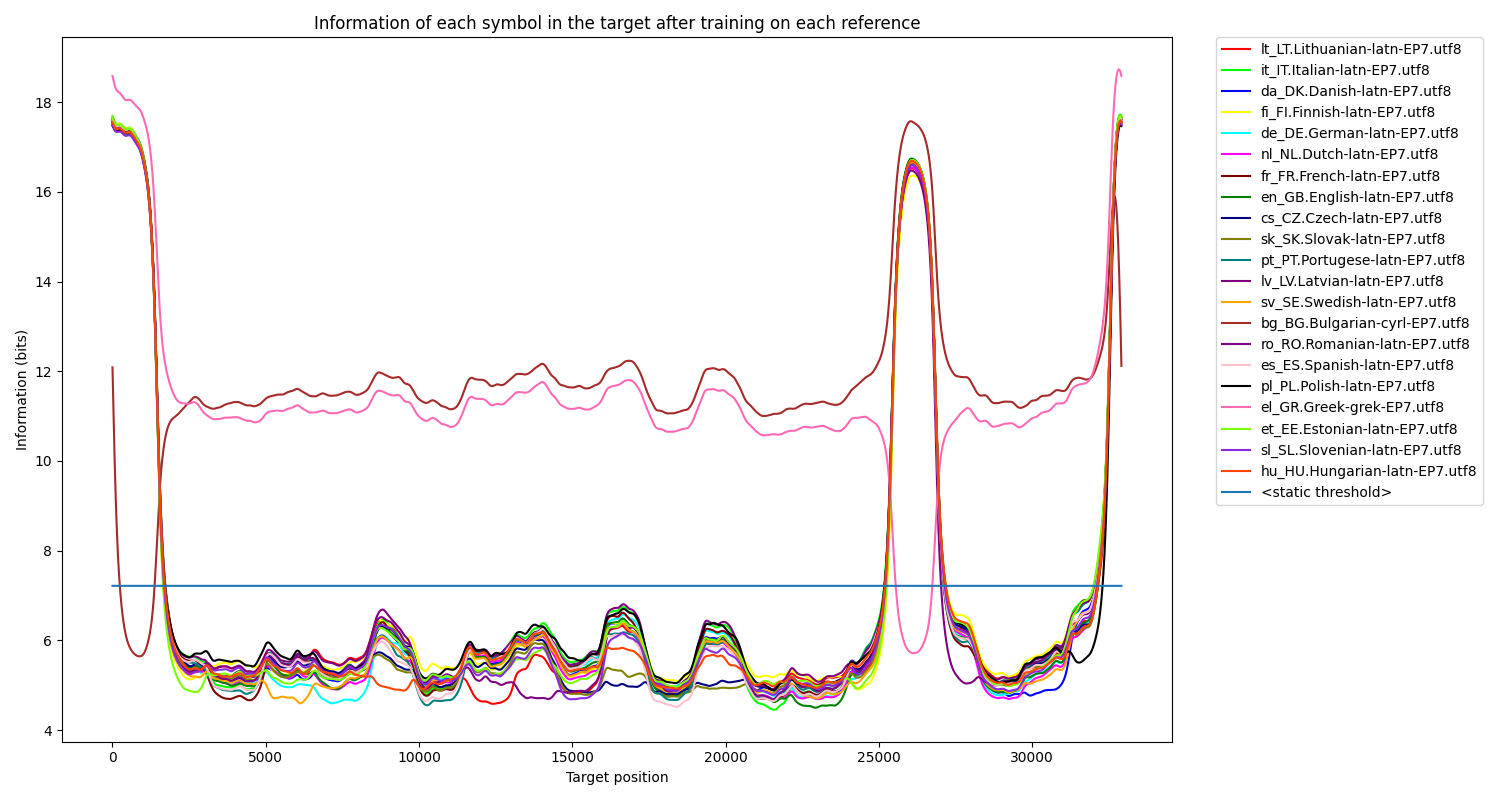
\includegraphics[width=0.95\textwidth]{../results/all_languages/-r_n.png}
    \caption{Information at each step for each language for \textit{all\_languages.txt}, newest pointer first.}
    \label{fig:all_languages_r_n}
\end{figure}

\begin{figure}
    \centering
    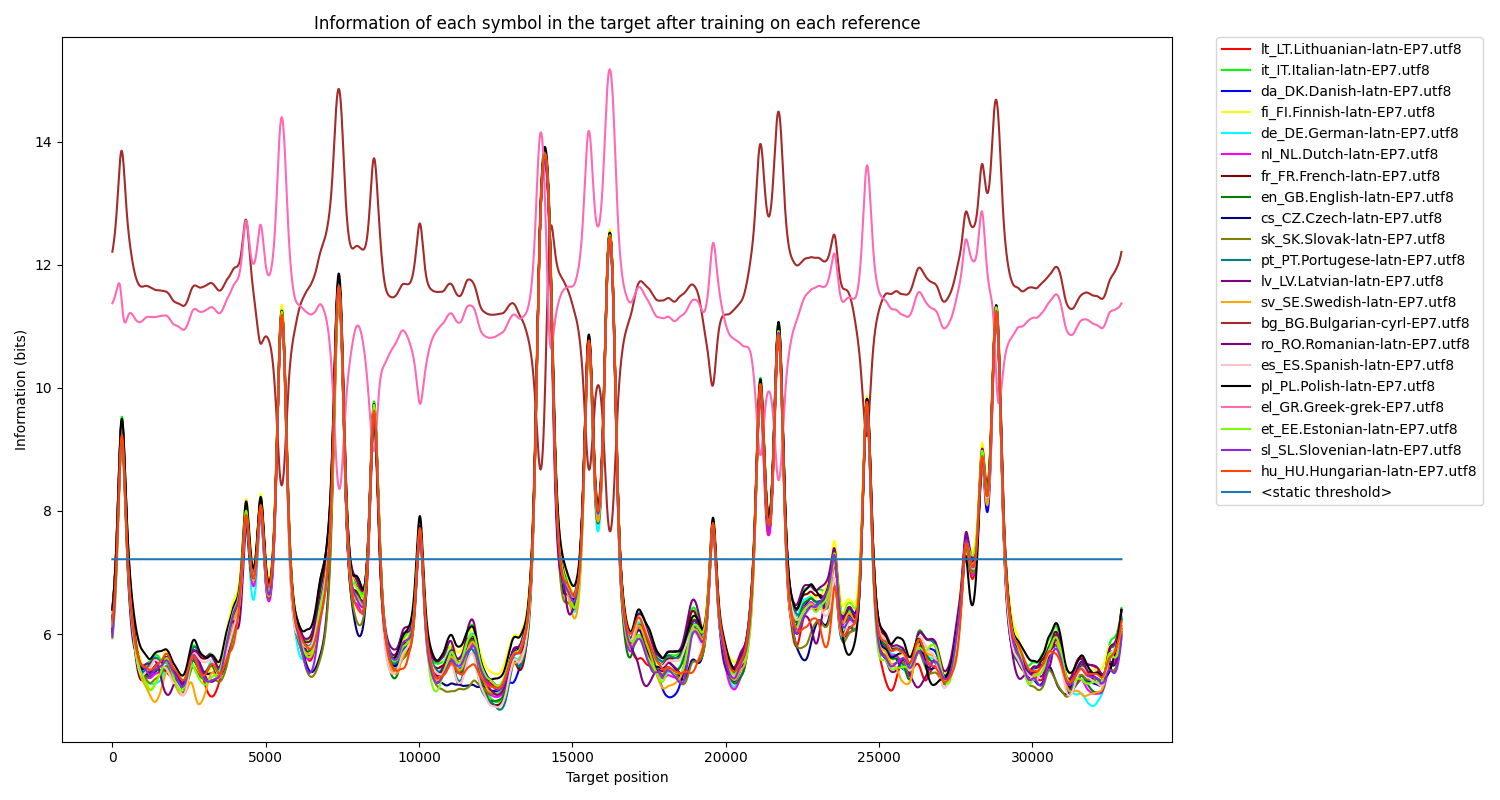
\includegraphics[width=0.95\textwidth]{../results/all_languages_random/-r_n.png}
    \caption{Information at each step for each language for \textit{all\_languages\_random.txt}, newest pointer first.}
    \label{fig:all_languages_random_r_n}
\end{figure}

\subsubsection{Copy pointer repositioning - Most common prediction}
\label{subsubsec:results_locate_lang_most_common_prediction}

In this case, the pointer chosen will be the one with the most common prediction.
Like the previous approaches, we can still distinguish the different languages, though the results are still identical, as we can see in the figures \ref{fig:all_languages_r_m} and \ref{fig:all_languages_random_r_m}.

\begin{figure}
    \centering
    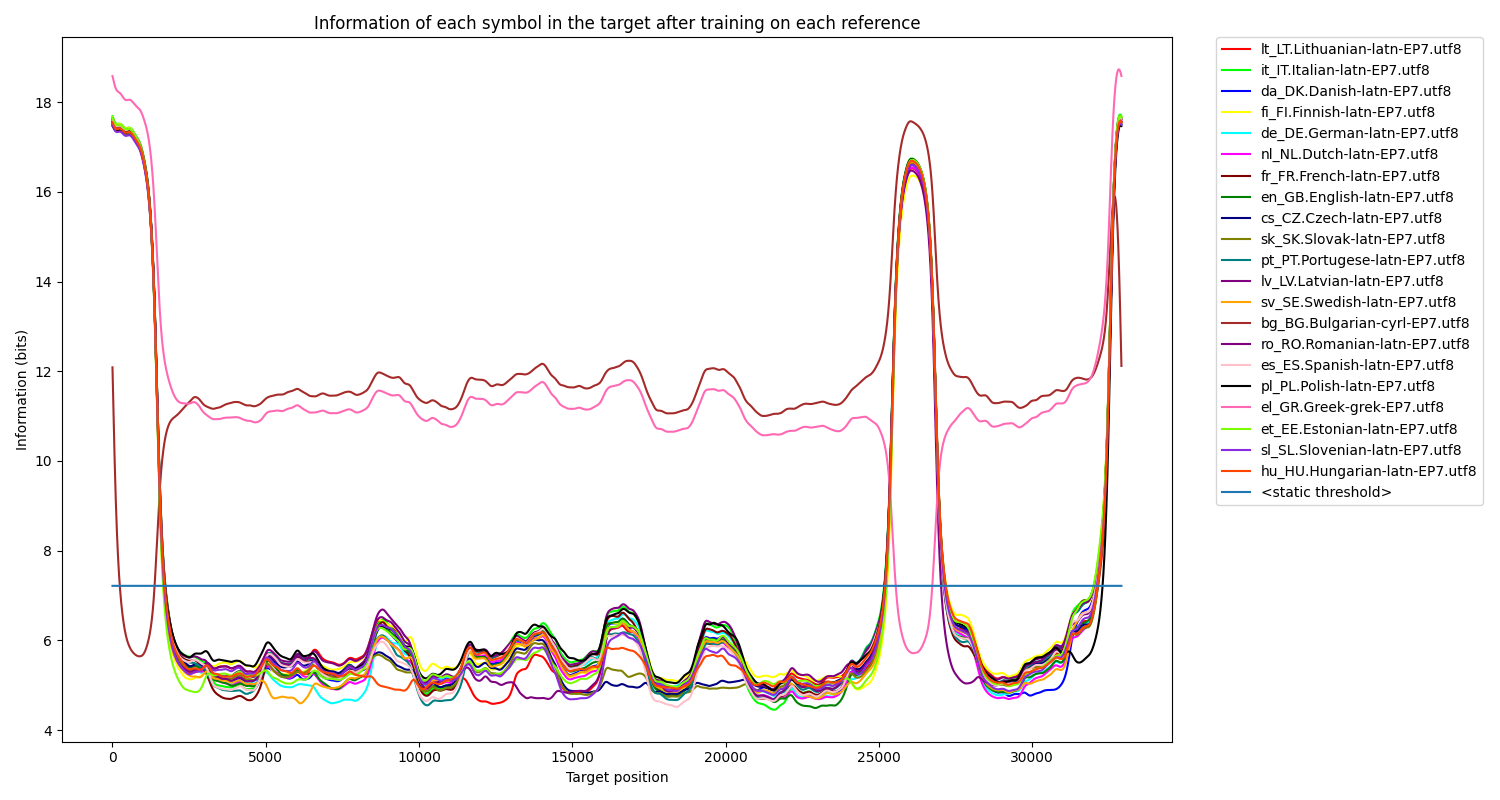
\includegraphics[width=0.95\textwidth]{../results/all_languages/-r_m.png}
    \caption{Information at each step for each language for \textit{all\_languages.txt}, most common prediction.}
    \label{fig:all_languages_r_m}
\end{figure}

\begin{figure}
    \centering
    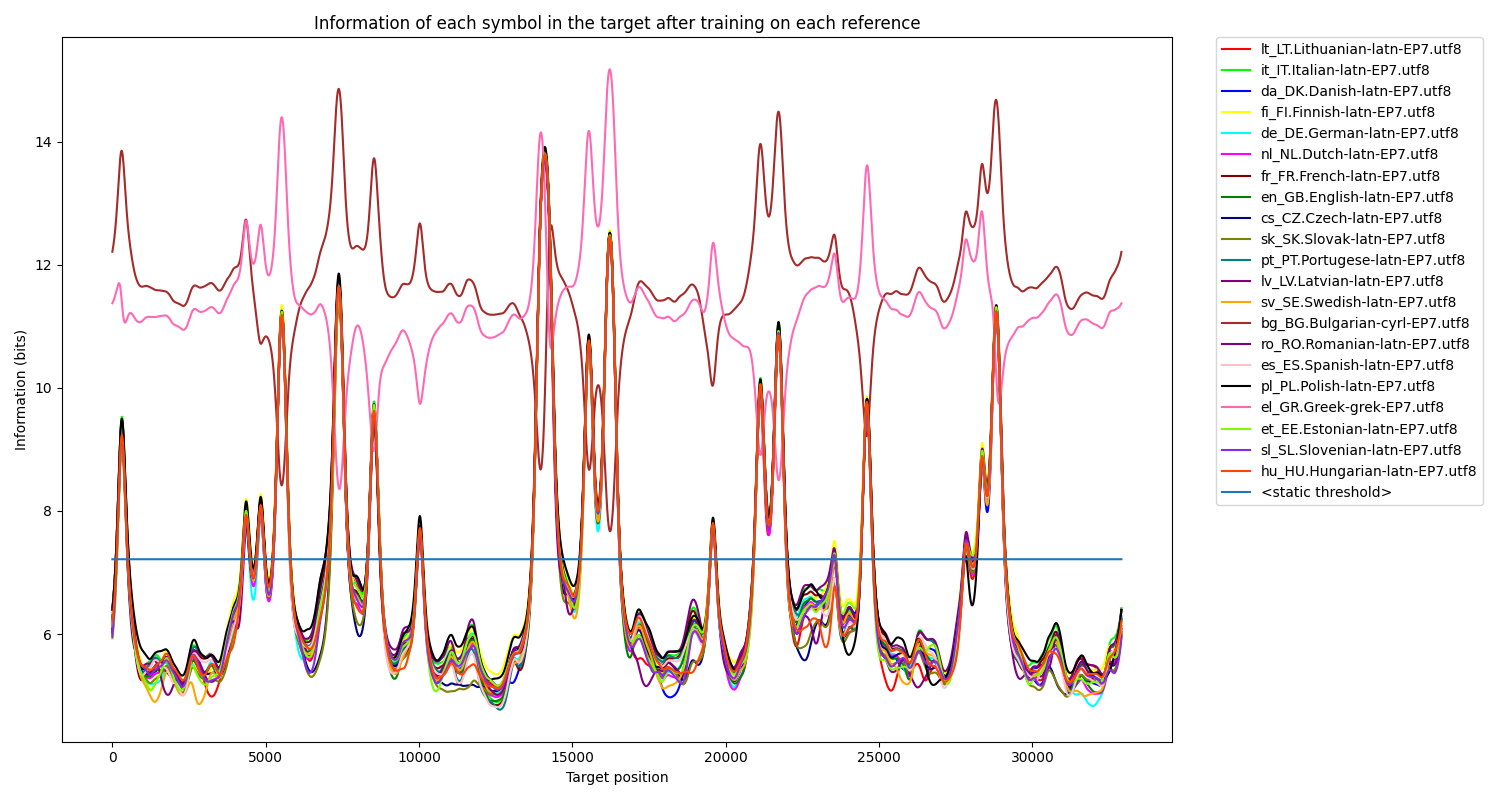
\includegraphics[width=0.95\textwidth]{../results/all_languages_random/-r_m.png}
    \caption{Information at each step for each language for \textit{all\_languages\_random.txt}, most common prediction.}
    \label{fig:all_languages_random_r_m}
\end{figure}

\subsubsection{Copy pointer repositioning - Most common prediction bounded}
\label{subsubsec:results_locate_lang_most_common_prediction_bounded}

This version of the most common prediction strategy is the same as the previous one, but with a bound on the number of most recent pointers that are considered.
For this test we used the best value for the size of the bound that we verified in the last assignment, which was $100$.
These results can be seen in the figures \ref{fig:all_languages_r_c} and \ref{fig:all_languages_random_r_c}, which are shown to be identical to the previous approaches.

\begin{figure}
    \centering
    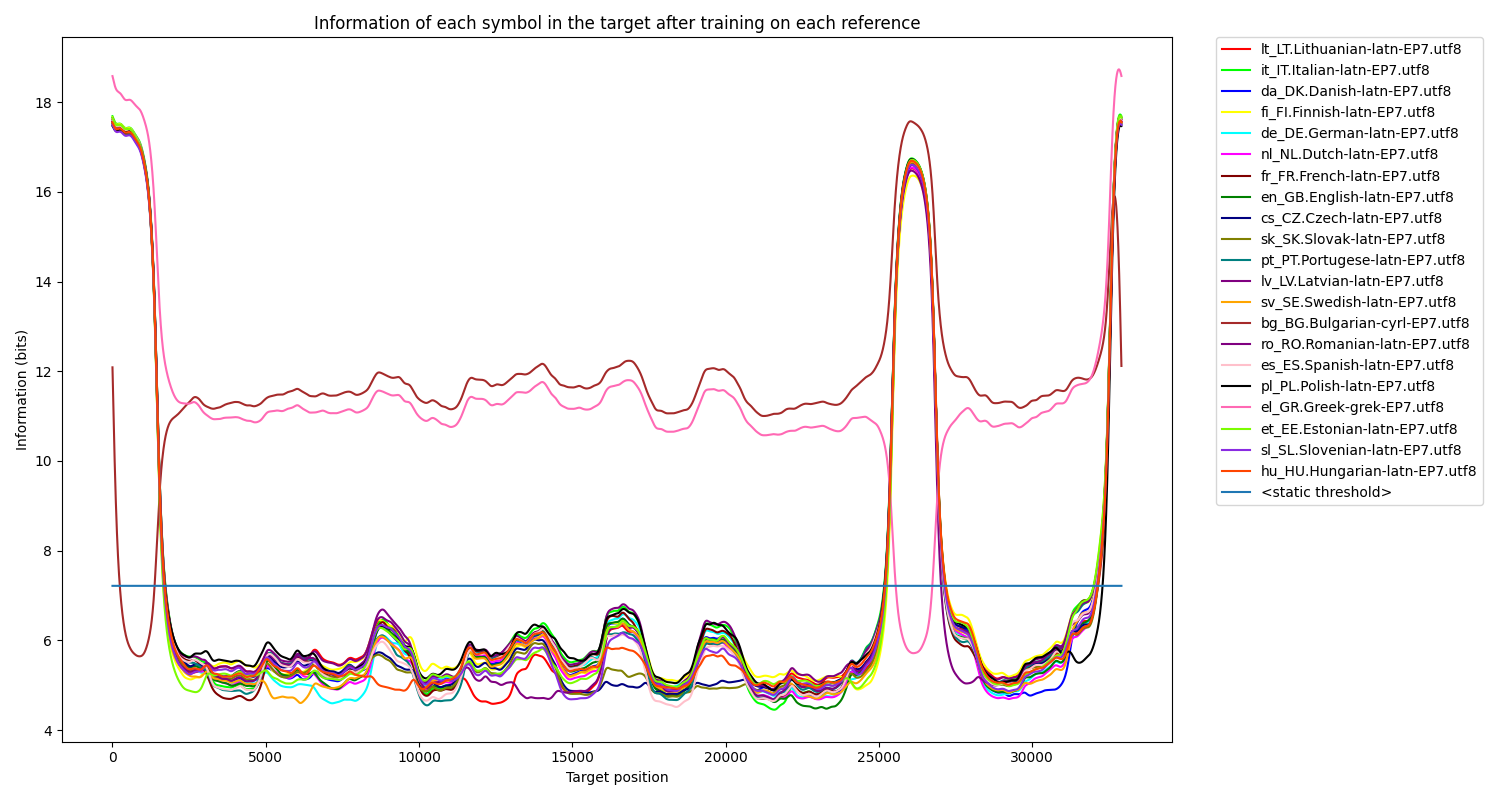
\includegraphics[width=0.95\textwidth]{../results/all_languages/-r_c:100.png}
    \caption{Information at each step for each language for \textit{all\_languages.txt}, most common prediction bounded.}
    \label{fig:all_languages_r_c}
\end{figure}

\begin{figure}
    \centering
    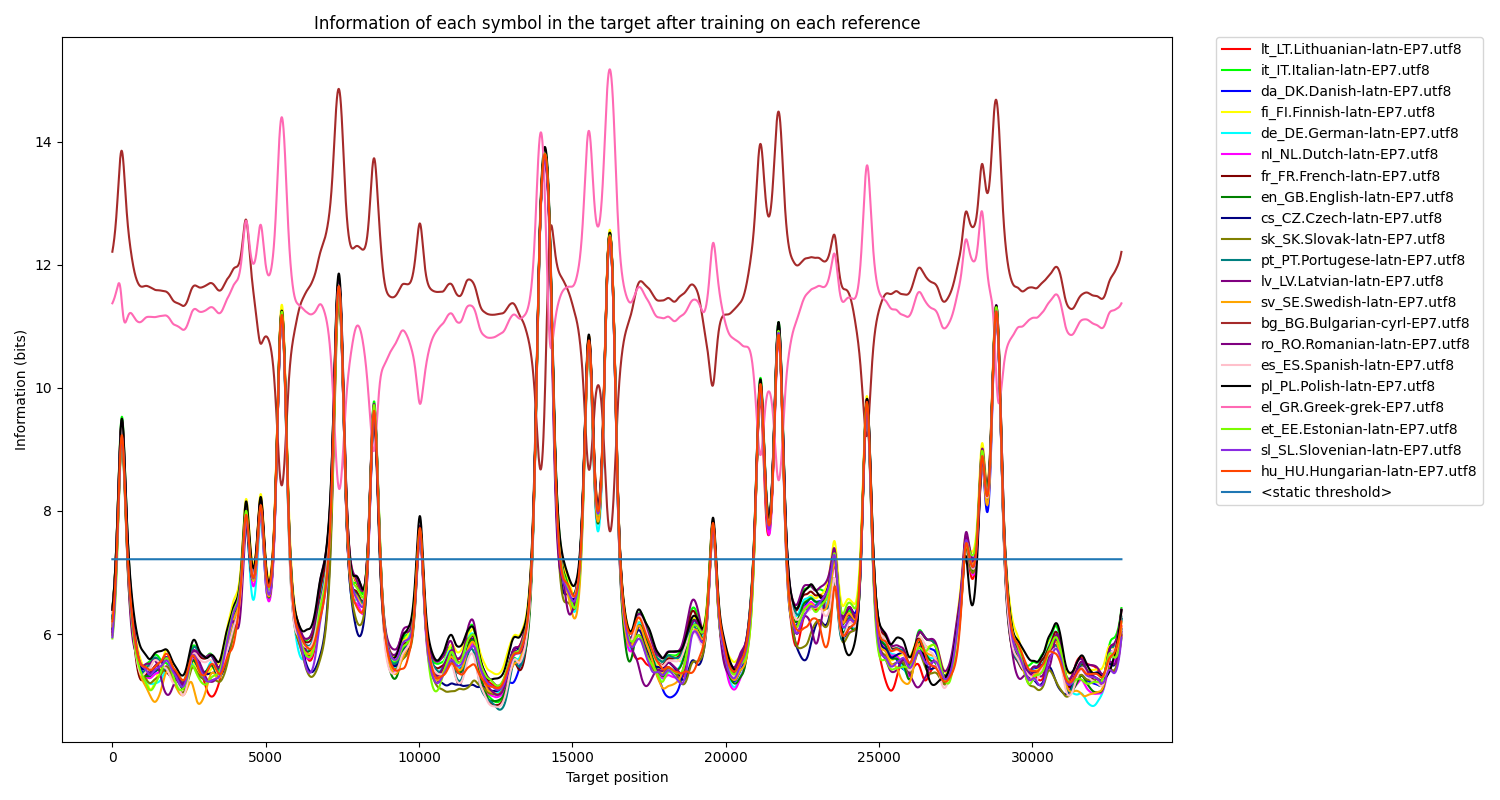
\includegraphics[width=0.95\textwidth]{../results/all_languages_random/-r_c:100.png}
    \caption{Information at each step for each language for \textit{all\_languages\_random.txt}, most common prediction bounded.}
    \label{fig:all_languages_random_r_c}
\end{figure}

\subsubsection{Copy pointer threshold - Static threshold}
\label{subsubsec:results_locate_lang_static_threshold}

Finally, we also tested the different threshold strategies, starting with the static threshold.
In this strategy, the threshold is set to a fixed value, which in this case is $0.5$ because it was the one which produced the lowest entropy values in the previous assignment.

In the figures \ref{fig:all_languages_t_n} and \ref{fig:all_languages_random_t_n}, we can see that the results are identical to the previous approaches.

\begin{figure}
    \centering
    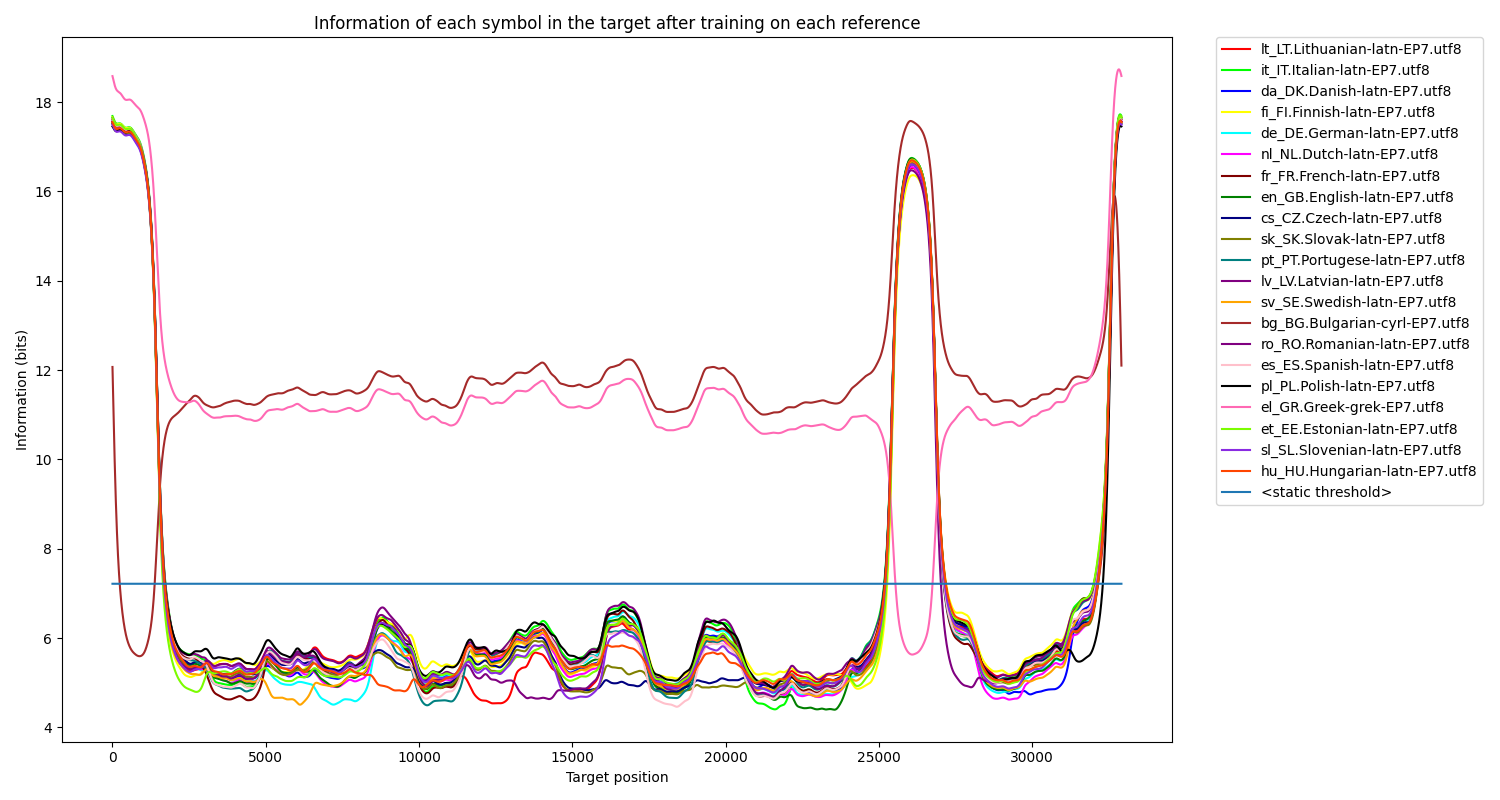
\includegraphics[width=0.95\textwidth]{../results/all_languages/-t_n:0.5.png}
    \caption{Information at each step for each language for \textit{all\_languages.txt}, static threshold.}
    \label{fig:all_languages_t_n}
\end{figure}

\begin{figure}
    \centering
    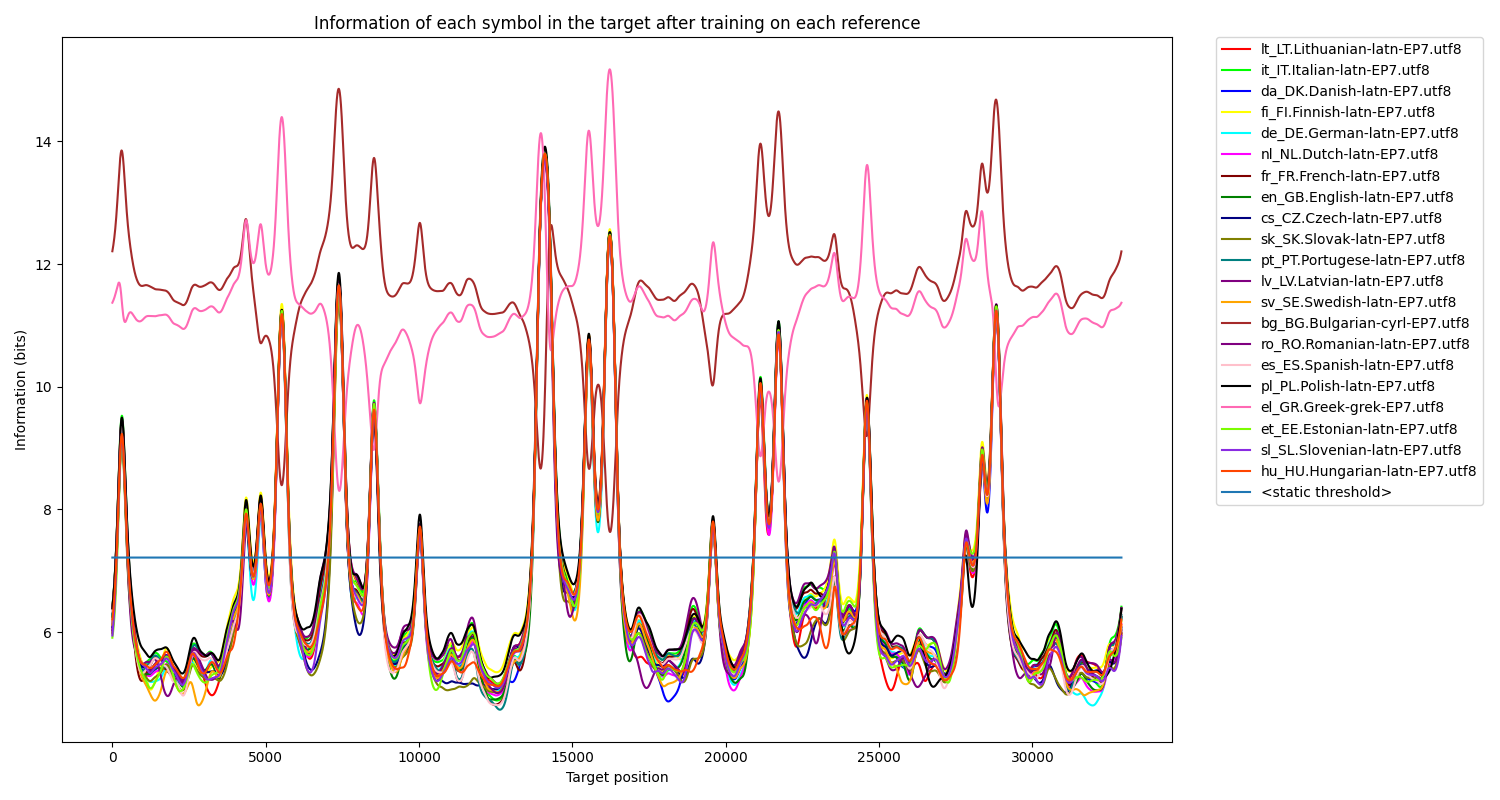
\includegraphics[width=0.95\textwidth]{../results/all_languages_random/-t_n:0.5.png}
    \caption{Information at each step for each language for \textit{all\_languages\_random.txt}, static threshold.}
    \label{fig:all_languages_random_t_n}
\end{figure}

\subsubsection{Copy pointer threshold - Successive fails threshold}
\label{subsubsec:results_locate_lang_successive_fails_threshold}

In this strategy, the threshold is set to a value that is calculated based on the number of successive prediction fails that the model has.
In this case, we used the value that we used in the previous assignment that produced better results, which was $9$.

The results are shown in figures \ref{fig:all_languages_t_f} and \ref{fig:all_languages_random_t_f}.
Interestingly, we can see that the results, although similar to the use of the static threshold,
show that the minimum information values are slightly higher, which correspond to the predicted language for the section.

\begin{figure}
    \centering
    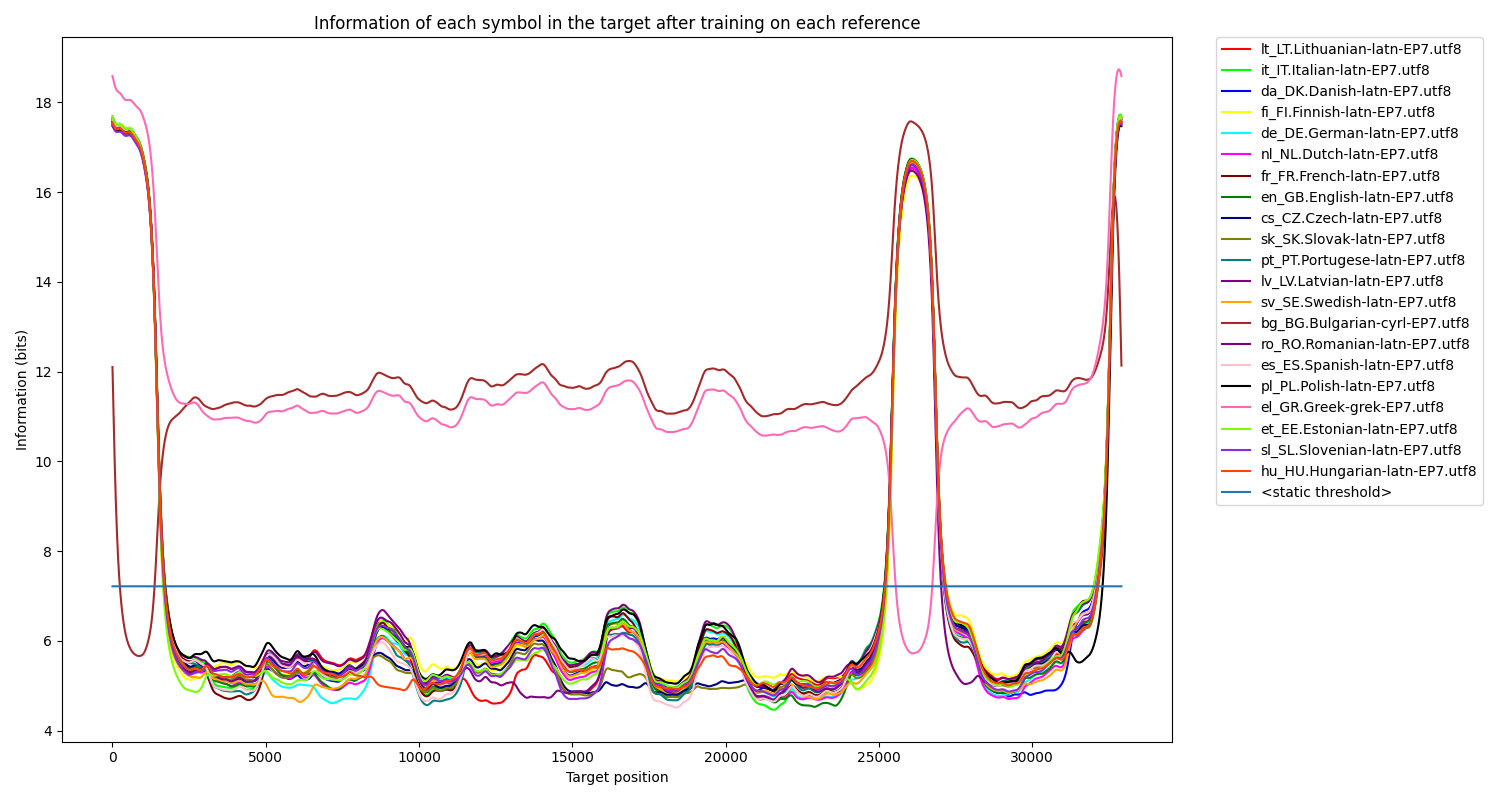
\includegraphics[width=0.95\textwidth]{../results/all_languages/-t_f:9.png}
    \caption{Information at each step for each language for \textit{all\_languages.txt}, successive fails threshold.}
    \label{fig:all_languages_t_f}
\end{figure}

\begin{figure}
    \centering
    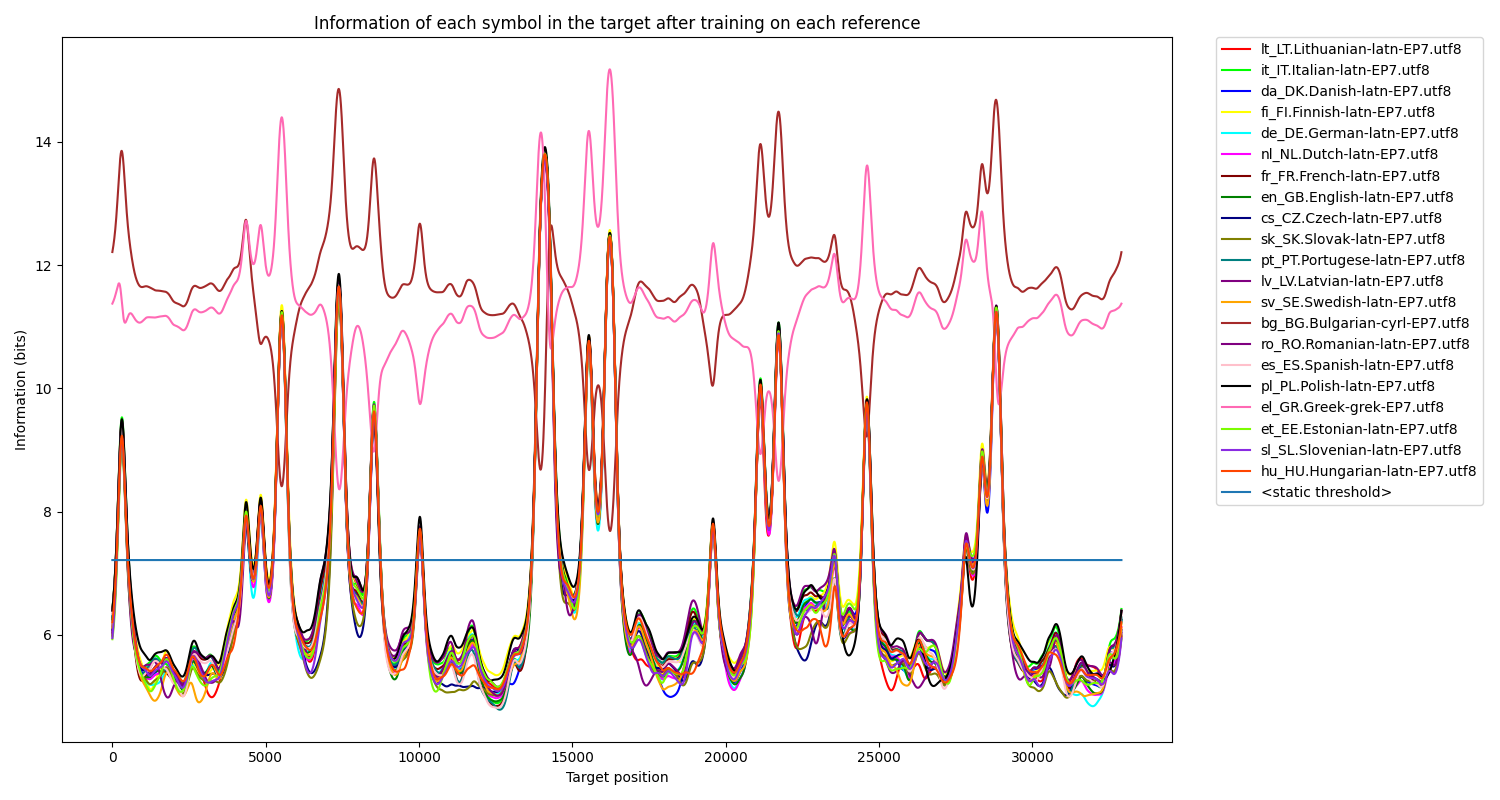
\includegraphics[width=0.95\textwidth]{../results/all_languages_random/-t_f:9.png}
    \caption{Information at each step for each language for \textit{all\_languages\_random.txt}, successive fails threshold.}
    \label{fig:all_languages_random_t_f}
\end{figure}

\subsubsection{Copy pointer threshold - Rate of change threshold}
\label{subsubsec:results_locate_lang_rate_of_change_threshold}

Finally, we tested the rate of change threshold strategy with the value $0.01$, which is the one that produced the best results in the previous assignment.

By observing figures \ref{fig:all_languages_t_c} and \ref{fig:all_languages_random_t_c}, we can see that the difference between the information values of the minimum reference
and second minimun reference is a bit higher than the previous threshold strategies, which means that the model is more confident in the prediction of the language of the section.
This makes this strategy the best one when choosing the threshold to switch pointers.

\begin{figure}
    \centering
    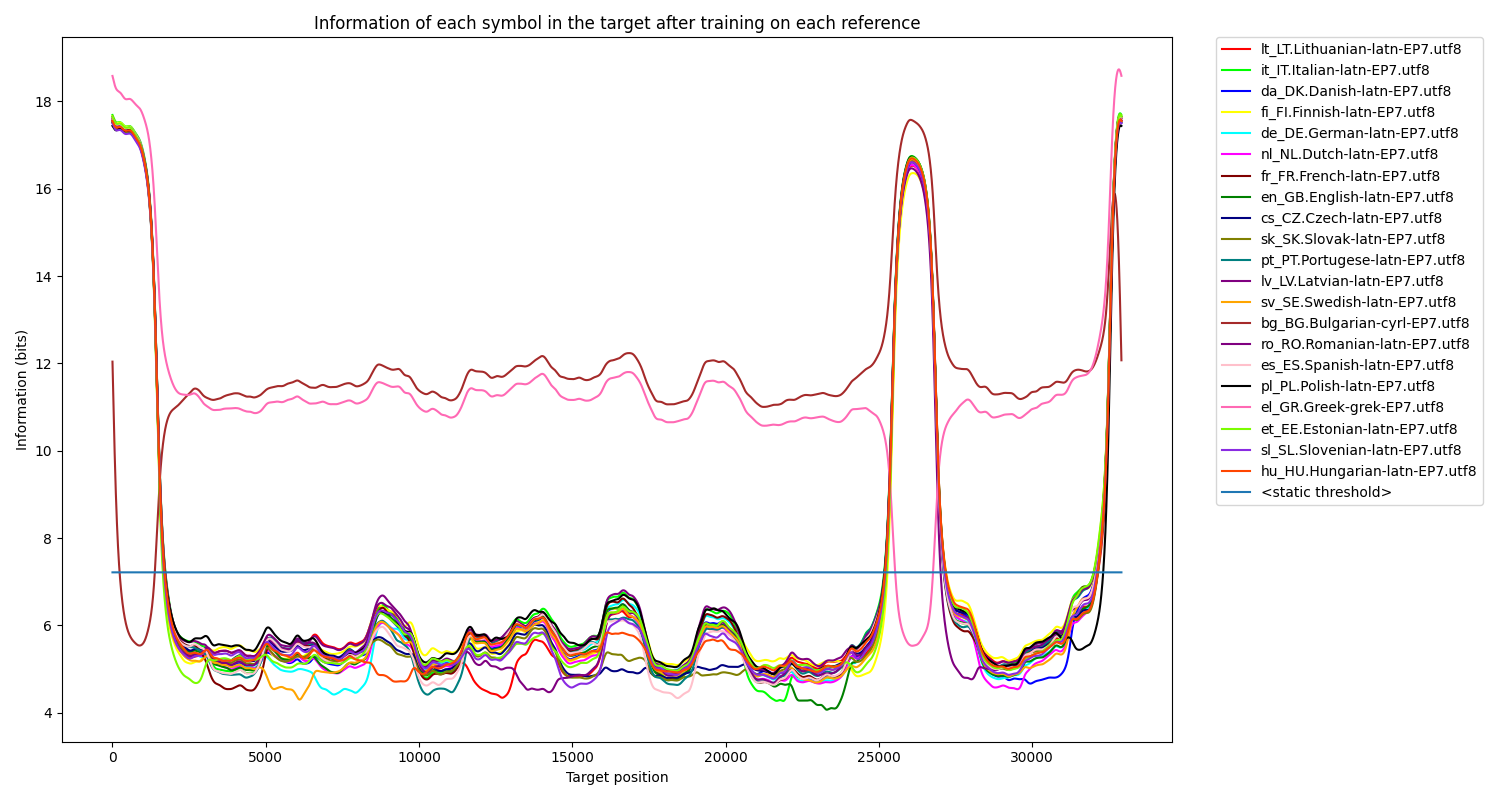
\includegraphics[width=0.95\textwidth]{../results/all_languages/-t_c:0.01.png}
    \caption{Information at each step for each language for \textit{all\_languages.txt}, rate of change threshold.}
    \label{fig:all_languages_t_c}
\end{figure}

\begin{figure}
    \centering
    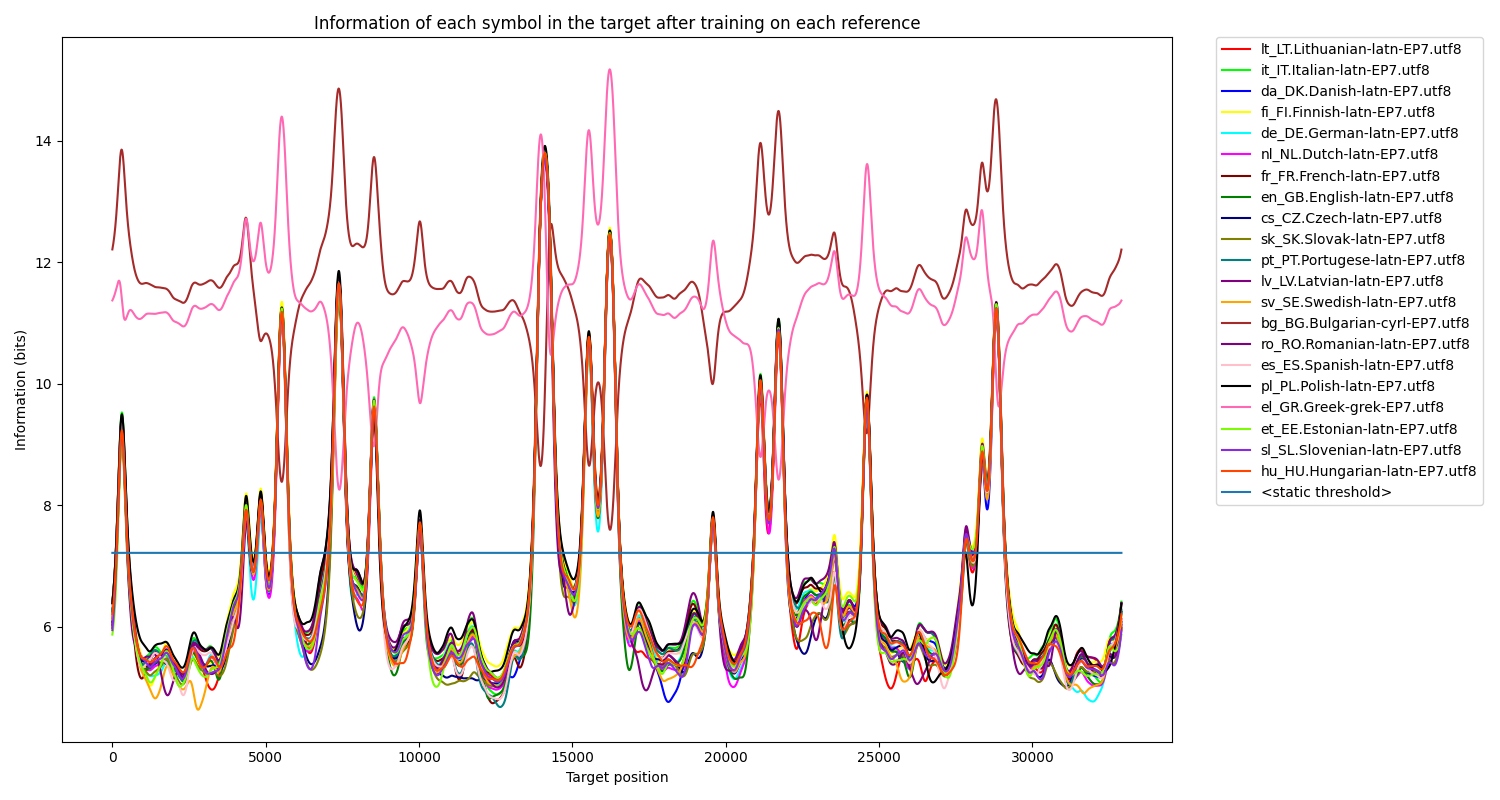
\includegraphics[width=0.95\textwidth]{../results/all_languages_random/-t_c:0.01.png}
    \caption{Information at each step for each language for \textit{all\_languages\_random.txt}, rate of change threshold.}
    \label{fig:all_languages_random_t_c}
\end{figure}


\subsubsection{Other parameters: Pattern size - k}
\label{subsubsec:results_locate_lang_pattern_size}

We also analyzed the effect of the context/pattern size $k$ on the language classification.
As we can see in figures \ref{fig:all_languages_k_3} and \ref{fig:all_languages_k_6} and \ref{fig:all_languages_k_9} 
the information values for the candidate language do decrease with the increase of the pattern size, but not in every case in the text file.
This change in information values is highly dependent on the text file and its language, although it seems better to use a bigger pattern size
because it also helps garantee that other languages are not possible candidates.

\begin{figure}
    \centering
    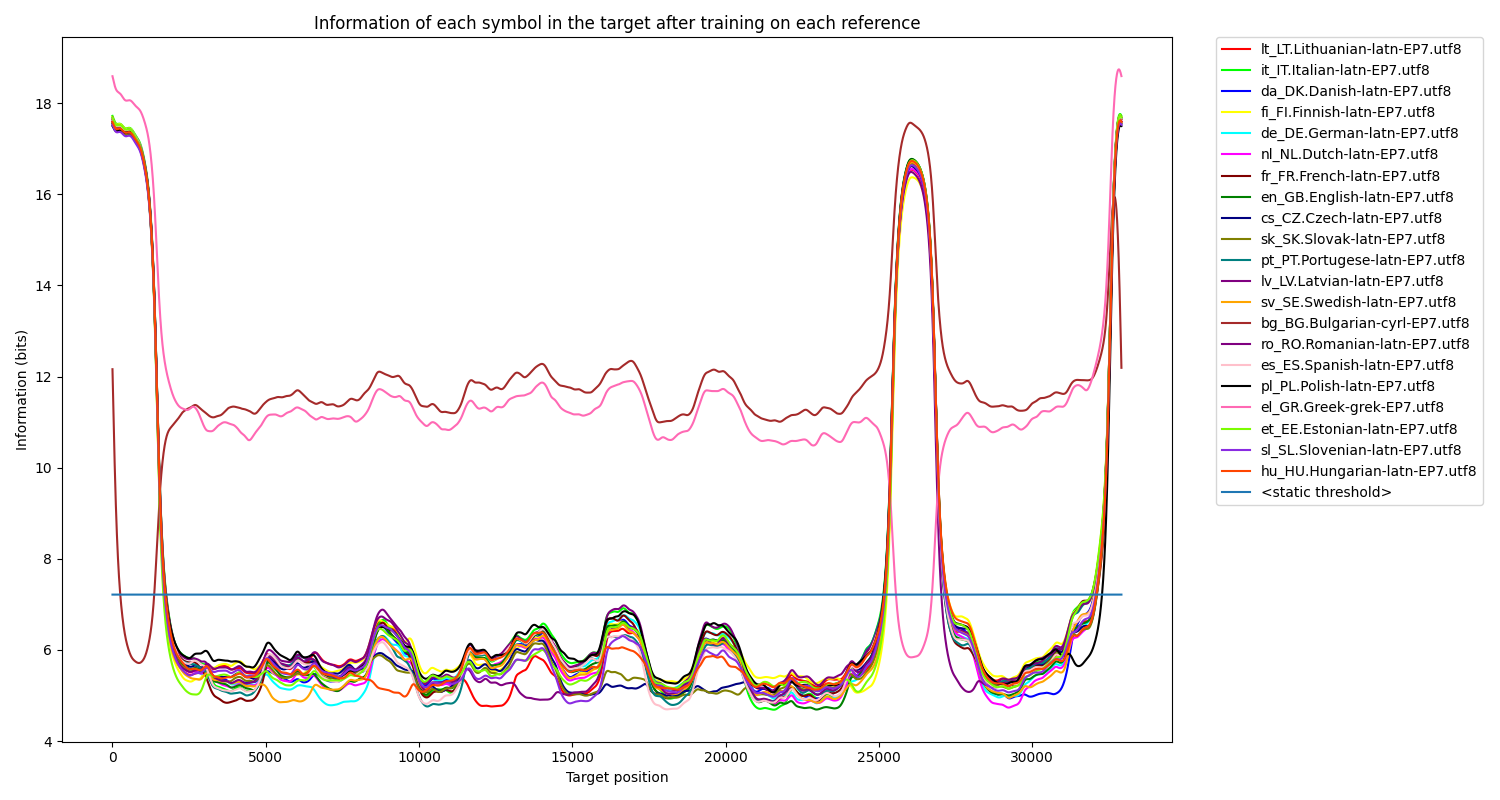
\includegraphics[width=0.95\textwidth]{../results/all_languages/-k_3_-a_1.png}
    \caption{Information at each step for each language for \textit{all\_languages.txt}, Pattern size 3.}
    \label{fig:all_languages_k_3}
\end{figure}

\begin{figure}
    \centering
    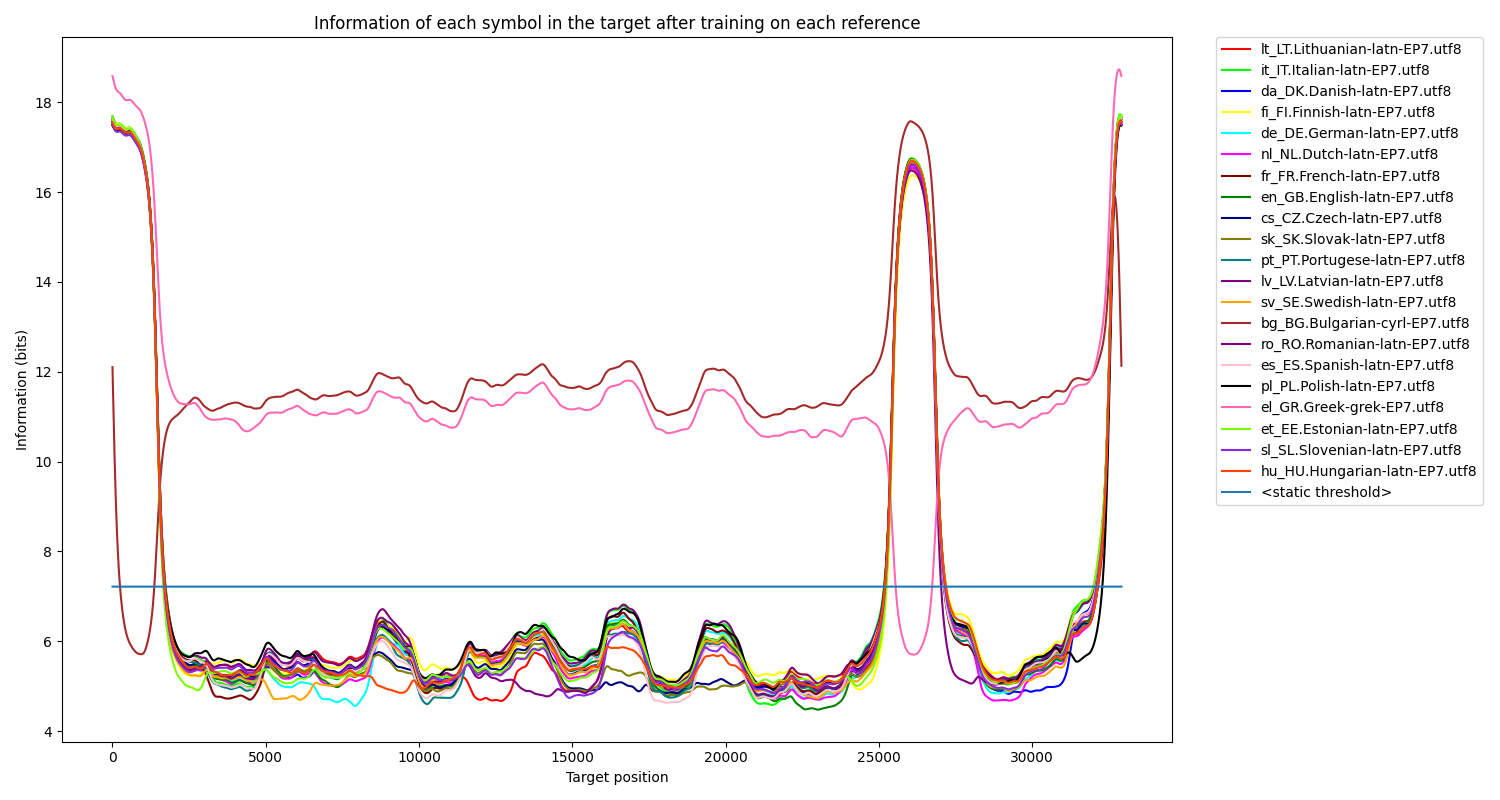
\includegraphics[width=0.95\textwidth]{../results/all_languages/-k_6_-a_1.png}
    \caption{Information at each step for each language for \textit{all\_languages.txt}, Pattern size 6.}
    \label{fig:all_languages_k_6}
\end{figure}

\begin{figure}
    \centering
    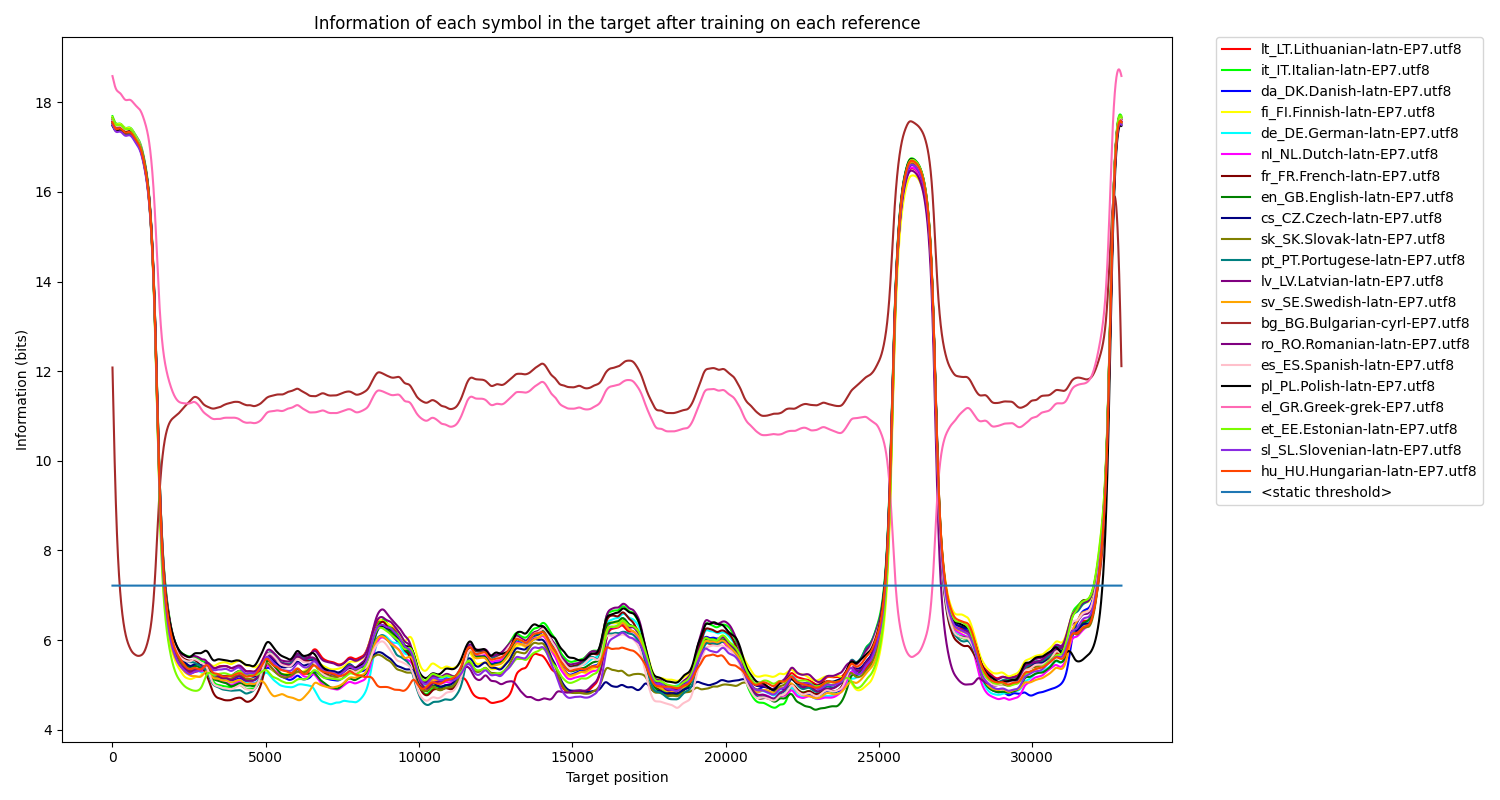
\includegraphics[width=0.95\textwidth]{../results/all_languages/-k_9_-a_1.png}
    \caption{Information at each step for each language for \textit{all\_languages.txt}, Pattern size 9.}
    \label{fig:all_languages_k_9}
\end{figure}


\subsubsection{Other parameters: Alpha - a}
\label{subsubsec:results_locate_lang_alpha}

We also analyzed the effect of the alpha parameter on the language classification.
By looking at the figures \ref{fig:all_languages_a0.5}, \ref{fig:all_languages_a1} and \ref{fig:all_languages_a10} we can see that the alpha parameter doesn't have a big impact on the results.
The only difference we can see is that the information values are slightly higher when using a bigger alpha value, which is expected since the alpha parameter is used to smoothen the probability distribution.
The exception are the values lower than 1, where the information values slightly change but do seemingly shift up or down like in the other cases.

\begin{figure}
    \centering
    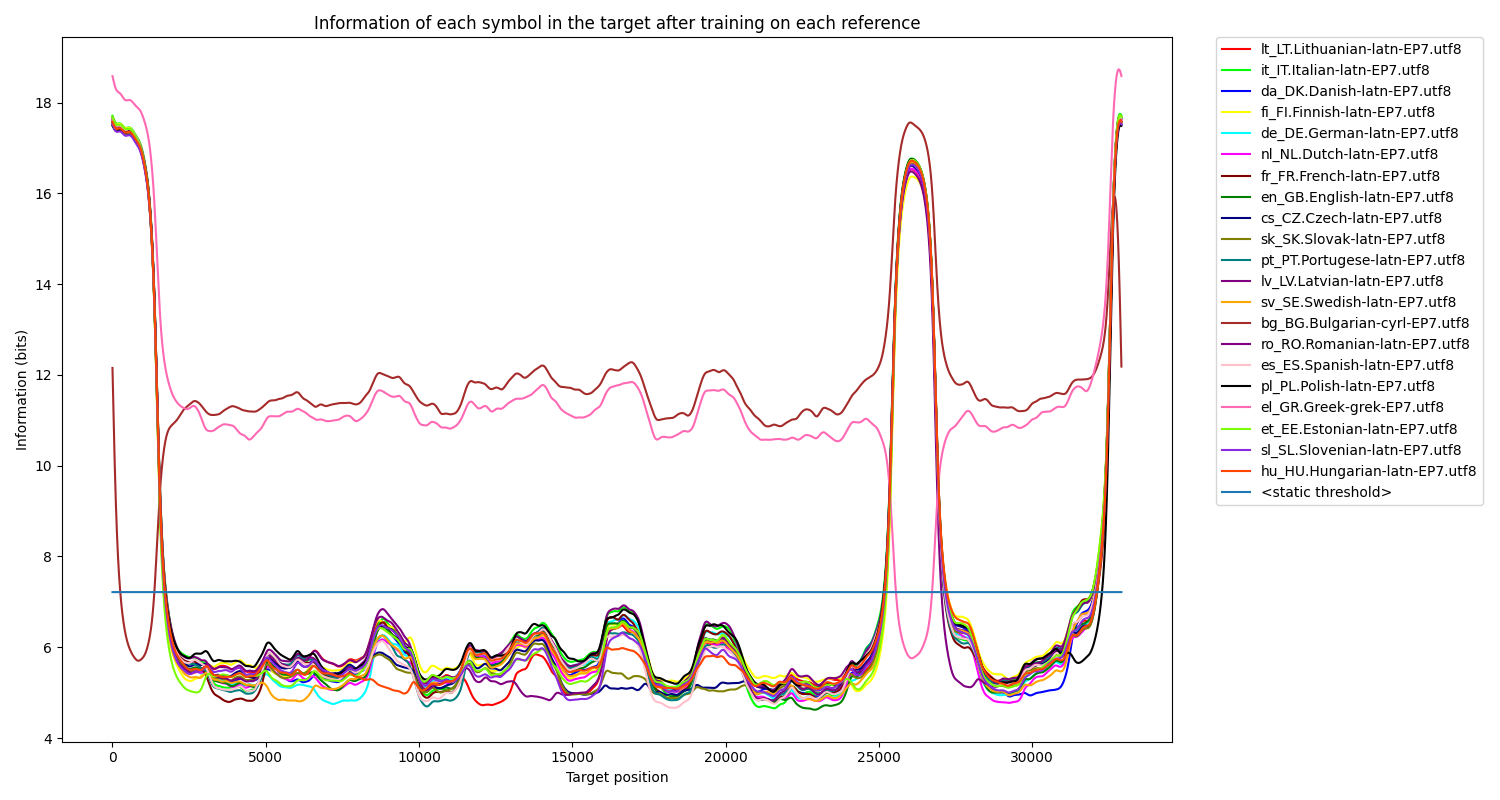
\includegraphics[width=0.95\textwidth]{../results/all_languages/-k_3_-a_0.5.png}
    \caption{Information at each step for each language for \textit{all\_languages.txt}, Alpha 0.5 and K=3.}
    \label{fig:all_languages_a0.5}
\end{figure}

\begin{figure}
    \centering
    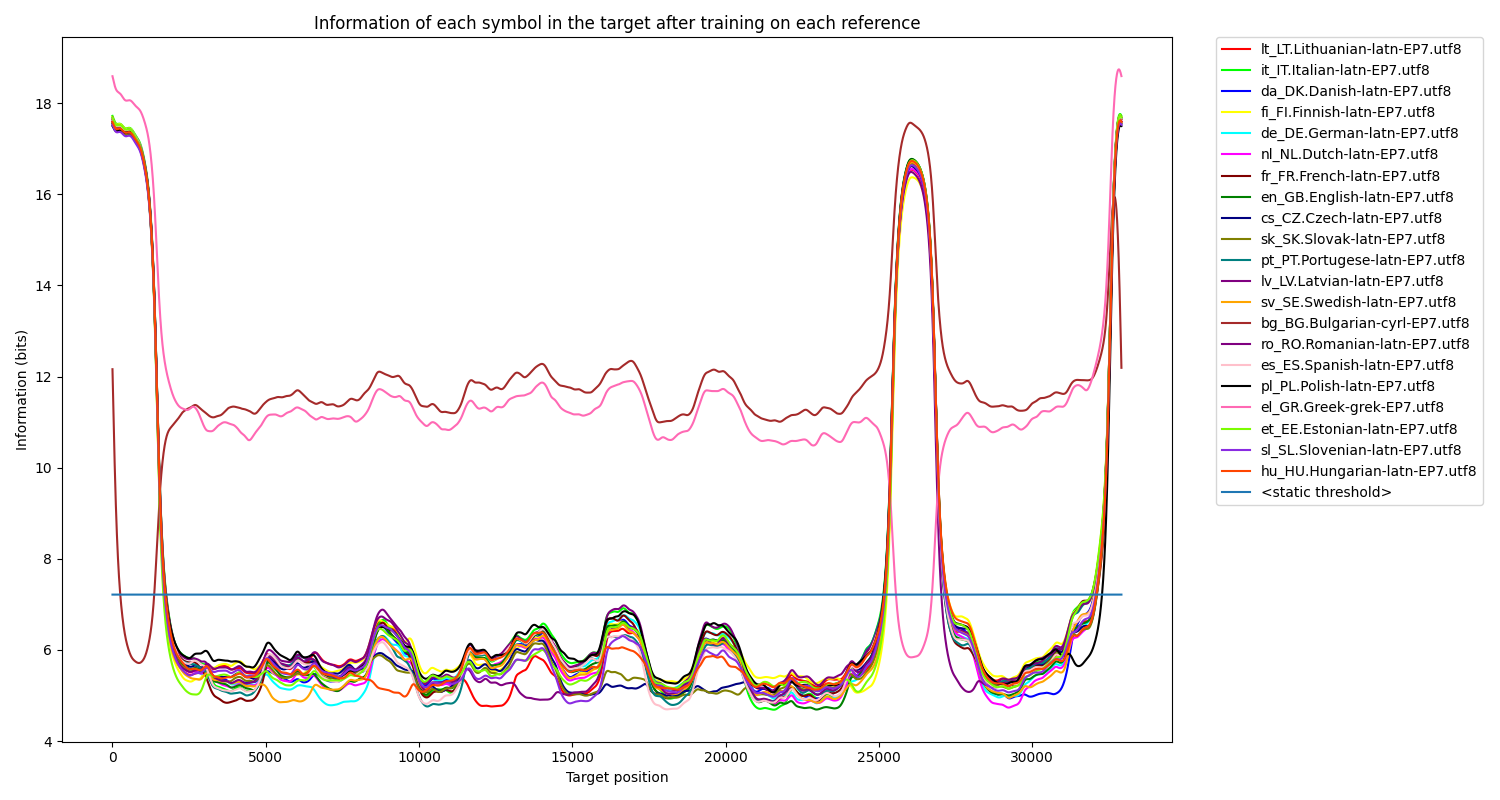
\includegraphics[width=0.95\textwidth]{../results/all_languages/-k_3_-a_1.png}
    \caption{Information at each step for each language for \textit{all\_languages.txt}, Alpha 1 and K=3.}
    \label{fig:all_languages_a1}
\end{figure}

\begin{figure}
    \centering
    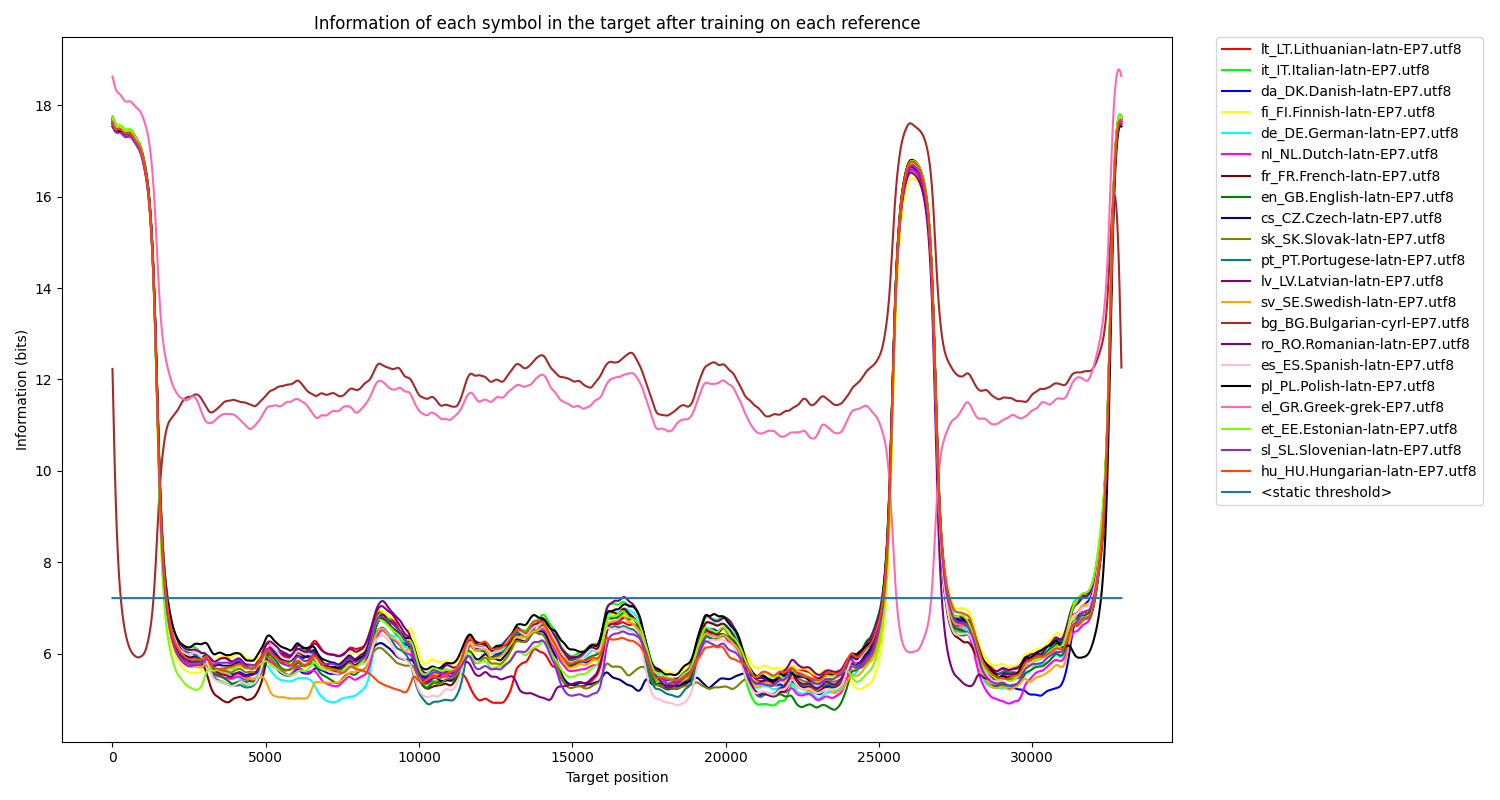
\includegraphics[width=0.95\textwidth]{../results/all_languages/-k_3_-a_10.png}
    \caption{Information at each step for each language for \textit{all\_languages.txt}, Alpha 10 and K=3.}
    \label{fig:all_languages_a10}
\end{figure}

\subsubsection{Accuracy dependent on lang model parameters}
\label{subsubsec:results_locate_lang_accuracy}

In this section we will analyze the accuracy of the \texttt{locate\_lang} script for different values of the \texttt{lang} model parameters.
The results are presented in table \ref{tab:locate_lang_accuracy}.

All the results are above 80\% accuracy, except for the last 2. This can be explained due to the fact that the static threshold is too low
although the difference between the information values of the most probable language and the second most probable language is still high like the other parameters.
If the static threshold wasn't taken into account, the accuracy of these cases would be much higher, probably close to the other cases. 
When using the finite-context model with small $\alpha$ and $k_f$, we notice a sizeable improvement in classification accuracy, with accuracy around 98\%.


\begin{table}
    \centering
    \begin{tabular}{|c|c|}
    \hline
    \textbf{Parameter} & \textbf{Accuracy (\%)} \\ \hline
    $p_c:10:3$ & 98.608579 \\ \hline
    $p_c:1:3$ & 98.572123 \\ \hline
    $t_c:0.01$ & 92.629724 \\ \hline
    $t_n:0.5$ & 91.703123 \\ \hline
    $k_3\_-a_{25}$ & 91.526917 \\ \hline
    $k_3\_-a_{50}$ & 91.526917 \\ \hline
    $k_3\_-a_{100}$ & 91.520841 \\ \hline
    $k_3\_-a_{10}$ & 91.511727 \\ \hline
    $k_3\_-a_5$ & 91.359825 \\ \hline
    $k_9\_-a_1$ & 91.043869 \\ \hline
    $r_n$ & 90.664115 \\ \hline
    $r_o$ & 90.661077 \\ \hline
    $r_m$ & 90.639810 \\ \hline
    $p_f$ & 90.639810 \\ \hline
    $r_c:100$ & 90.636772 \\ \hline
    $k_9\_-a_{0.5}$ & 90.980070 \\ \hline
    $k_9\_-a_5$ & 90.402844 \\ \hline
    $t_f:9$ & 90.144611 \\ \hline
    $k_6\_-a_{0.5}$ & 90.023089 \\ \hline
    $k_9\_-a_{10}$ & 89.865111 \\ \hline
    $k_3\_-a_1$ & 89.755742 \\ \hline
    $k_6\_-a_5$ & 89.011423 \\ \hline
    $k_9\_-a_{25}$ & 88.795722 \\ \hline
    $k_9\_-a_{50}$ & 88.546603 \\ \hline
    $k_9\_-a_{100}$ & 88.403816 \\ \hline
    $k_6\_-a_{10}$ & 88.139507 \\ \hline
    $k_6\_-a_{25}$ & 86.374408 \\ \hline
    $k_6\_-a_{50}$ & 85.496415 \\ \hline
    $k_6\_-a_{100}$ & 85.037672 \\ \hline
    $p_c:100:3$ & 84.062462 \\ \hline
    $p_c:1:9$ & 3.821850 \\ \hline
    $p_u$ & 1.108883 \\ \hline
    \end{tabular}
    \caption{Accuracy of the \texttt{locate\_lang} script for different values of the parameters.}
    \label{tab:locate_lang_accuracy}
\end{table}

\subsubsection{Processing parameters - Frequency dropoff}
\label{subsubsec:results_locate_lang_frequency_dropoff}

In terms of the \texttt{locate\_lang} processing parameters, figures \ref{fig:ll_f_all_languages} and \ref{fig:ll_f_dog} present the effect of the frequency dropoff, i.e. the strength of the low-pass filter, for the \textit{all\_languages.txt} and \textit{dog.txt} target files on the classification accuracy.
As can be seen from the plots, there is an ideal range of values for the frequency dropoff, below which the accuracy is very low and above which the accuracy doesn't increase.
In this case, we can notice that a frequency dropoff value of around 50 already provides great classification accuracy.

Note that if the frequency dropoff is 0, then it is equivalent to having no low-pass filter applied.
Therefore, we can see the heavy influence of the low-pass filter, as applying just some filtering brings the accuracy from $40\%$ without any filter to above $90\%$.
As explained in section \ref{subsec:methodology_locate_lang}, the copy model's behaviour is very erratic, with spurious and short copies throughout the target text.
As such, it is understandable that a low-pass filter heavily improves the classification accuracy, since these spikes of information are attenuated and so we can better study trends over larger segments of the target text instead of symbol-by-symbol.

\begin{figure}
    \centering
    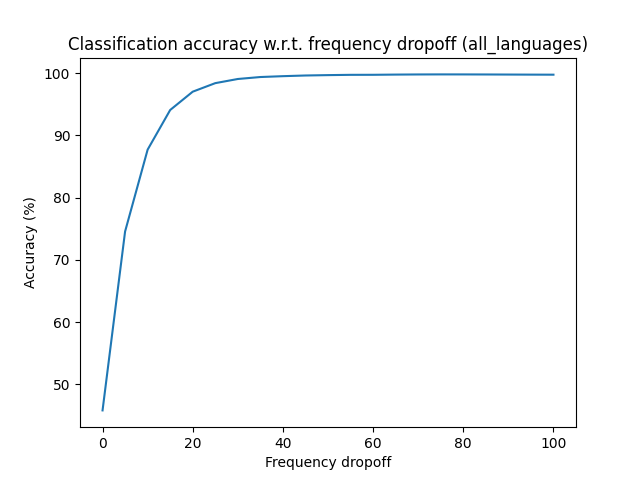
\includegraphics[width=0.85\textwidth]{../results/all_languages/ll-f.png}
    \caption{Accuracy with respect to \texttt{locate\_lang}'s frequency dropoff value, on \textit{all\_languages.txt}.}
    \label{fig:ll_f_all_languages}
\end{figure}

\begin{figure}
    \centering
    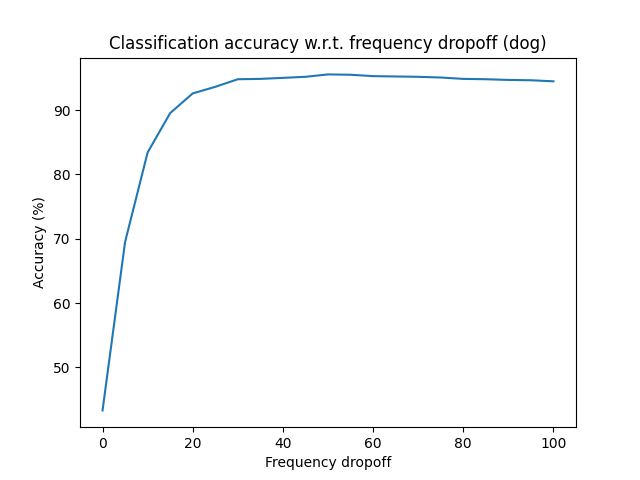
\includegraphics[width=0.85\textwidth]{../results/dog/ll-f.png}
    \caption{Accuracy with respect to \texttt{locate\_lang}'s frequency dropoff value, on \textit{dog.txt}.}
    \label{fig:ll_f_dog}
\end{figure}

\subsubsection{Processing parameters - Minimum threshold}
\label{subsubsec:results_locate_lang_minimum_threshold}

The minimum threshold dictates how similar is the minimum reference allowed to be to the second minimum reference.
We tested values below or equal to $1.0$, with $1.0$ meaning that the minimum reference can report exactly the same information as the second minimum at a given step.
Technically, if the minimum threshold is $1.0$, then it has no effect.
Figures \ref{fig:ll_m_all_languages} and \ref{fig:ll_m_dog} present the effect of this parameter on the classification accuracy.

From the plots, we can notice that minimum threshold values below $1.0$ decrease the classification accuracy.
In the \textit{dog.txt} target the curve is more irregular, but still decreasing.
Although the threshold was conceived to reduce ambiguity in the target language when many were likely candidates, it ended up heavily reducing classification performance overall.
The reason that likely prevented the program from classifying correctly with this threshold is the transition between languages in the target text.
In these transitional sections, the program labels the symbols as unknown since there is confusion, whereas without any threshold the program tries to make a best effort to classify the perceived language, without reporting any unknowns.

\begin{figure}
    \centering
    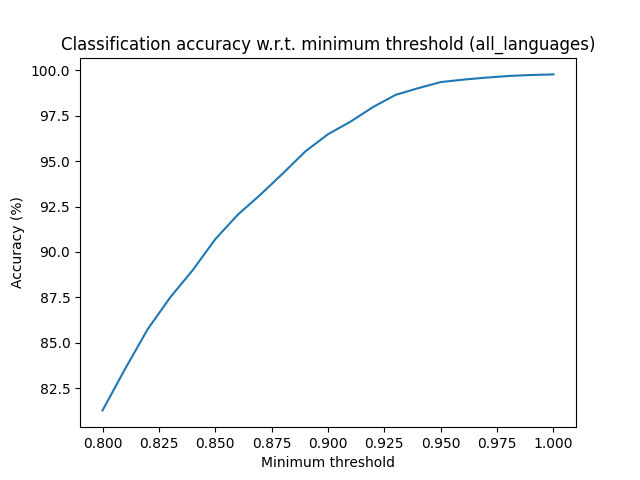
\includegraphics[width=0.85\textwidth]{../results/all_languages/ll-m.png}
    \caption{Accuracy with respect to \texttt{locate\_lang}'s minimum threshold, on \textit{all\_languages.txt}.}
    \label{fig:ll_m_all_languages}
\end{figure}

\begin{figure}
    \centering
    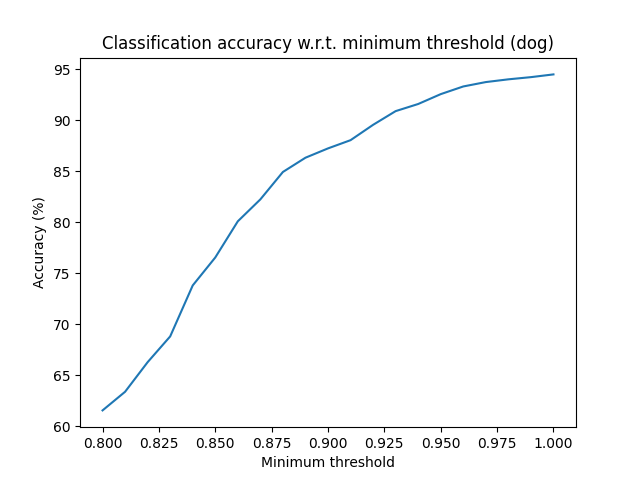
\includegraphics[width=0.85\textwidth]{../results/dog/ll-m.png}
    \caption{Accuracy with respect to \texttt{locate\_lang}'s minimum threshold, on \textit{dog.txt}.}
    \label{fig:ll_m_dog}
\end{figure}

\subsubsection{Processing parameters - Static threshold}
\label{subsubsec:results_locate_lang_static_threshold_processing}

The \texttt{locate\_lang}'s static threshold defines a maximum value below which a reference's reported information should be to be considered.
More specifically, the parameter value passed to \texttt{locate\_lang} defines the denominator $\gamma$ in equation \ref{eq:locate_lang_static_threshold}, described in section \ref{subsec:methodology_locate_lang}.
We tested different values of $\gamma$ above $1.0$.
As previously explained, $\gamma = 1.0$ defines a static threshold that demands a compression performance at least better than reporting a uniform distribution at each step.
In practice, if we consider for instance the uniform distribution and the probability distribution based on a finite-context model, then $\gamma = 1.0$ is as if no threshold was applied at all.
Figures \ref{fig:ll_s_all_languages} and \ref{fig:ll_s_dog} present the classification accuracy with respect to the denominator $\gamma$ of the static threshold.

We can notice that there is a local maximum for both targets.
Around $\gamma = 1.2$, we can see that the classification accuracy is the highest, and the larger the value the lower it gets.
Curiously, for the \textit{dog.txt} target the classification accuracy is particularly worse for $\gamma = 1.0$ than it is for $\gamma = 1.2$.
This makes sense when we consider the purpose of the static threshold.
Since the threshold was conceived so that we can identify languages that we may not have trained on, i.e. are not in the reference bank, then if we set $\gamma = 1.0$ there will be effectively no threshold.
As such, we can't identify unknown languages at all.
Since both targets have a section in Chinese, which does not have a respective reference, then this section will be guaranteedly misclassified for both targets if $\gamma = 1.0$.
The effect is more pronounced in \textit{dog.txt} since the portion that Chinese occupies in the file is larger than in \textit{all\_languages.txt}.

Additionally, if $\gamma$ increases too much, then we are demanding a better performance from the copy model.
At this point, it is better to tune this value such that it properly represents the compression performance of the copy model, which we found to be around $1.2$.

\begin{figure}
    \centering
    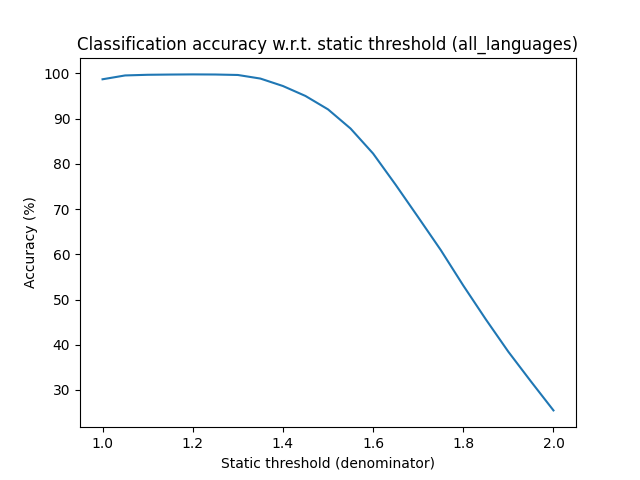
\includegraphics[width=0.85\textwidth]{../results/all_languages/ll-s.png}
    \caption{Accuracy with respect to \texttt{locate\_lang}'s static threshold, on \textit{all\_languages.txt}.}
    \label{fig:ll_s_all_languages}
\end{figure}

\begin{figure}
    \centering
    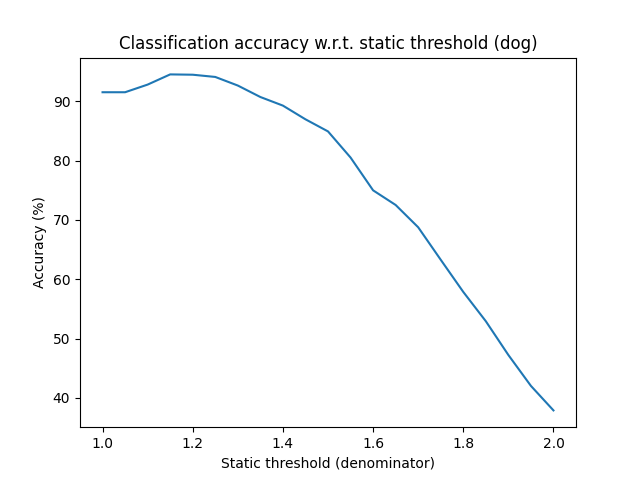
\includegraphics[width=0.85\textwidth]{../results/dog/ll-s.png}
    \caption{Accuracy with respect to \texttt{locate\_lang}'s static threshold, on \textit{dog.txt}.}
    \label{fig:ll_s_dog}
\end{figure}

\subsubsection{Variable reference size}
\label{subsubsec:results_locate_lang_variable_reference_size}

We also analyzed the effect of the reference's size on the language classification.
As we can see in tables \ref{tab:rel_size_ref_acc_dog} and \ref{tab:rel_size_ref_acc_all} the accuracy of the language classification increases with the size of the reference.
This was the expected behavior since the model has more information to work with and therefore a more complete and complex model.
Although we must admit that we weren't expecting such a high accuracy with a reference of only 10\% of the original reference files.
With these results we can conclude that the model is robust and can work with small references.

To test this we used the \textit{dog.txt} and \textit{all\_languages.txt} files as the target file, the references were made randomly with lines from the original 
reference files. The size of the reference was varied from 10\% to 100\% with increments of 10\%, of the original reference files.

\begin{table}
    \centering
    \begin{tabular}{|l|l|}
    \hline
        Size of the reference (\%) & Accuracy (\%) \\ \hline
        0.1 & 90.885891 \\ \hline
        0.2 & 97.760967 \\ \hline
        0.3 & 99.273909 \\ \hline
        0.4 & 99.659740 \\ \hline
        0.5 & 99.732653 \\ \hline
        0.6 & 99.750881 \\ \hline
        0.7 & 99.753919 \\ \hline
        0.8 & 99.766071 \\ \hline
        0.9 & 99.778223 \\ \hline
        1.0 & 99.781261 \\ \hline
    \end{tabular}
    \caption{Relation between the size of the reference and the accuracy of the language classification on the \textit{all\_languages.txt} file.}
    \label{tab:rel_size_ref_acc_all}
\end{table}

\begin{table}
    \centering
    \begin{tabular}{|l|l|}
    \hline
        Size of the reference (\%) & Accuracy (\%) \\ \hline
        10 & 87.117552 \\ \hline
        20 & 92.431562 \\ \hline
        30 & 93.666130 \\ \hline
        40 & 93.880837 \\ \hline
        50 & 93.988191 \\ \hline
        60 & 93.988191 \\ \hline
        70 & 94.202899 \\ \hline
        80 & 94.202899 \\ \hline
        90 & 94.310252 \\ \hline
        100 & 94.471283 \\ \hline
    \end{tabular}
    \caption{Relation between the size of the reference and the accuracy of the language classification on the \textit{dog.txt} file.}
    \label{tab:rel_size_ref_acc_dog}
\end{table}

We can also conclude that the accuracy of the language classification is affected by the size of the target file, 
a bigger target file will have a higher accuracy.
This happens because the language segments are bigger for \textit{all\_languages.txt}, giving more time for the model to find a context with a past from which to start copying.
In \textit{dog.txt}, the segments are shorter, requiring the copy model to transition between languages more often.

\section{Conclusion}
\label{sec:conclusion}

With the development of this assignment, we were able to conclude that our \texttt{lang} model
produces good results overall in both scripts developed with some variations dependending on the
parameters used, specially when changing to the finite-context model approach.

\subsection{Find lang}
\label{subsec:conclusion:find_lang}

Through the analysis of the results, we can conclude that the best approach to find the language of a text is to use the finite-context model.
Using the frequency and uniform distribution strategies did also correctly identify the language of all target texts tested, although with considerably lower confidence values.
In contrast, the finite-context model produced much better results with confidence values not lower than $77.3\%$ when testing with the target texts.
Another big improvement between the frequency and uniform distribution strategies and the finite-context model is the fact that the latter has a much better capacity to confirm
that it can't identify a language when it is not present in the references, which is a very important feature. For the frequency and uniform distribution strategies, the confidence
value for the Chinese text was $37.7\%$ for a different language, which is even higher than some correct predictions previously made. In contrast, the finite context model produced a
confidence value of $0.0\%$ for the same text, which is the expected result, and guarantees that the model is not making a wrong prediction.

\subsection{Locate lang}
\label{subsec:conclusion:locate_lang}

In the case of the \texttt{locate\_lang} script, the results were also very positive overall, with the model being able to correctly identify the language of the sections of the target texts,
with special emphasis when using the finite-context approach, which had a bigger difference in reported information between the correct language and the second most probable language.

By testing the different parameters, we verified that most of the \texttt{lang} parameters had a very small impact on the results, due to the different nature of the objective between this
assignment and the previous one. The only parameter that had a significant impact on the results was the threshold strategy, with the rate of change threshold strategy producing
slightly better results than the other two strategies, by creating a slightly bigger difference between the reported information values of the correct language and the second most probable language.

In terms of the script's processing parameters, we found that the minimum threshold did not improve the classification accuracy at all, and that both the $\gamma$ parameter for the static threshold and the frequency dropoff values had optimal values that provided local maximums in terms of classification accuracy.

\section{References}
\bibliography{refs}
\bibliographystyle{IEEEtran}

\end{document}
